%\documentclass[article]{jss}
\documentclass[nojss]{jss}

% Just for editing
%\usepackage{setspace}
%\doublespacing

%% -- LaTeX packages and custom commands ---------------------------------------

\usepackage{marginnote}
\newcommand{\revmarginnote}[1]{{\reversemarginpar\marginnote{#1}}}

% prevent "widows" and "orphans" in regular text paragraphs:
\widowpenalty10000
\clubpenalty10000
% prevent orphans for section headings:
%\usepackage[nobottomtitles]{titlesec} % doesn't work: breaks the code
%\usepackage[all]{nowidow}
% Couldn't find a solution... Just use \newpage at problematic headings, for now.
% These include:
% - 2.6: Spatio-temporal framework
% - 3.2: Example: Non-Gaussian, areally-referenced spatial data and change-of-support
% - 3.3: Increased numbers of basis functions in FRK v2

% Same indentation over multiple lines in algorithm environment: use tabularx to figure out the width of a box that would fit until the end of the line:
\usepackage{tabularx}
\makeatletter
\newcommand{\multiline}[1]{%
  \begin{tabularx}{\dimexpr\linewidth-\ALG@thistlm}[t]{@{}X@{}}
    #1
  \end{tabularx}
}
\makeatother

%% algorithm environments
\usepackage{algpseudocode,algorithm,algorithmicx}
\newcommand*\Let[2]{\State #1 $\gets$ #2}
\algrenewcommand\algorithmicrequire{\textbf{Precondition:}}
\algrenewcommand\algorithmicensure{\textbf{Postcondition:}}


\usepackage{siunitx} % si units

% ---- Text mode commands ----
\newcommand{\red}[1]{\textcolor{red}{#1}} 
\newcommand{\blue}[1]{\textcolor{blue}{#1}} 
\definecolor{darkgreen}{rgb}{0.0, 0.5, 0.0}
\newcommand{\green}[1]{\textcolor{darkgreen}{#1}} 
\usepackage{layouts} % \printinunitsof to get the size of \textwidth and \linewidth

% ---- Math mode commands ----

\usepackage{rotating} % \rotatebox

\usepackage{amsmath}	% align environment.
\usepackage{amsfonts}	% \mathbb{} (used for Real number symbol, etc.)
\usepackage{amsthm}		% mathy stuff (Theorems, Lemmas, etc.)
%\usepackage{amssymb}     % re-define \emptyset to look nice
%\let\emptyset\varnothing % re-define \emptyset to look nice
\usepackage{commath}
\usepackage{bbm} % \mathbb{} doesn't support digits (1, 2, 3, etc.), so use \mathbbm{} in these instances
\usepackage{mathtools} % \vdotswithin command to have vertical dots between equals signs

%% Lists
\usepackage{enumerate}

%% Formatting tables
\usepackage{pbox} % formatting cells with a table (forced line break within a cell)
\usepackage{multirow}
\newenvironment{tabnote}{\par\footnotesize}{\par}

%% recommended packages
\usepackage{thumbpdf,lmodern}

%% another package (only for this demo article)
\usepackage{framed}

%% new custom commands
\newcommand{\class}[1]{`\code{#1}'}
\newcommand{\fct}[1]{\code{#1()}}

%% Nice boldface math
\def\mbf#1{{%         \mbf{X} makes X a math bold letter
\mathchoice%          selects with respect to current style
{\hbox{\boldmath$\displaystyle{#1}$}}%      case 1 is displaystyle
{\hbox{\boldmath$\textstyle{#1}$}}%         case 2 is textstyle
{\hbox{\boldmath$\scriptstyle{#1}$}}%       case 3 is scriptstyle
{\hbox{\boldmath$\scriptscriptstyle{#1}$}}% case 4 is scriptscriptstyle
}}
\def\vec{\mbf}


%% General maths commands
\newcommand{\lr}[1]{\left(#1\right)} 
\def\d{\textrm{d}} % Define the "d" for use in integrals.
\newcommand{\logit}[1]{\text{logit}\!\left(#1\right)} % logit function
\newcommand{\logistic}[1]{\text{logistic}\!\left(#1\right)} % logistic function
\DeclareMathOperator*{\argmax}{arg\,max} % argmax
\DeclareMathOperator*{\argmin}{arg\,min} % argmin
\DeclareMathOperator{\Lagr}{\mathcal{L}} % Lagrangian L
\newcommand\numberthis{\addtocounter{equation}{1}\tag{\theequation}} % number within align*
\newcommand{\explr}[1]{\exp\!\left(#1\right)} % exp function with brackets (makes converting between e^{#1} and exp(#1) extremely easy)
\newcommand{\lnlr}[1]{\ln\!\left(#1\right)} % ln function with brackets 
\newcommand{\loglr}[1]{\log\!\left(#1\right)} % ln function with brackets 

%% General stats commands 
\newcommand{\Gau}{{\text{Gau}}}
\def\inddist{\:\stackrel{\text{ind}}{\sim}\:}
\newcommand{\simiid}{\overset{\text{iid}}{\sim}}
\renewcommand{\E}[1]{\mathbb{E}(#1)} % Expectation operator
\newcommand{\ENoLR}[1]{\mathbb{E}(#1)} % Expectation operator
\newcommand{\ECurly}[1]{\mathbb{E}\left\{#1\right\}} % Expec operator, curly brackets
\newcommand{\ESquare}[1]{\mathbb{E}\left[#1\right]} % Expec operator, square brackets
\newcommand{\var}[1]{{\rm var\!}\left(#1\right)} % variance operator
\newcommand{\precision}[1]{{\rm prec}\left(#1\right)} % precision operator
\newcommand{\precisionNoLR}[1]{{\rm prec}(#1)} % precision operator
\newcommand{\varCurly}[1]{{\rm var}\left\{#1\right\}} % variance operator, curly brackets
\newcommand{\varSquare}[1]{{\rm var}\left[#1\right]} % variance operator, square brackets 
\newcommand{\cov}[2]{{\rm cov\!}\left(#1,\, #2\right)} % covariance operator
\newcommand{\covCurly}[2]{{\rm cov}\left\{#1,\;\; #2\right\}} % covariance operator, curly brackets
\newcommand{\covCurlyConditional}[3]{{\rm cov}\left\{#1,\; #2 \mid #3\right\}} % covariance operator, curly brackets
\newcommand{\covSquare}[2]{{\rm cov}\left[#1,\;\; #2\right]} % covariance operator, square brackets
\newcommand{\indep}{\rotatebox[origin=c]{90}{$\models$}} % Independent Symbol: \indep

%% Linear algebra commands
\newcommand{\rank}[1]{{\rm rank}\left(#1\right)}
\newcommand{\tr}[1]{{\rm tr}\left(#1\right)}
\newcommand{\tp}{{\!\scriptscriptstyle \top}}
\newcommand{\vecFN}[1]{{\rm vec \!}\left(#1\right)} % vec operator
\newcommand{\diag}[1]{\text{diag}\left(#1\right)} % diag function: \diag

%% Predictor and MSPE definitions 
\newcommand{\pYgivenZ}[1]{\hat{p}_{Y|\vec{Z}}\left(#1\right)} 
\newcommand{\pmugivenZ}[1]{\hat{p}_{\mu|\vec{Z}}\left(#1\right)} 
\newcommand{\pmugivenZApprox}[1]{\check{p}_{\mu|\vec{Z}}\left(#1\right)} 
\newcommand{\pZgivenZ}[1]{\hat{p}_{Z|\vec{Z}}\left(#1\right)} 
\newcommand{\MSPE}[1]{\text{MSPE}\left\{#1\right\}} 
\newcommand{\MSPEtwoarg}[2]{\text{MSPE}\left\{#1, #2\right\}} 


%% Define a \hat{} that will fit over any function input. 
\usepackage{scalerel,stackengine}
\usepackage{scalerel}
\stackMath
\newcommand\reallywidehat[1]{%
\savestack{\tmpbox}{\stretchto{%
  \scaleto{%
    \scalerel*[\widthof{\ensuremath{#1}}]{\kern-.6pt\bigwedge\kern-.6pt}%
    {\rule[-\textheight/2]{1ex}{\textheight}}%WIDTH-LIMITED BIG WEDGE
  }{\textheight}% 
}{0.5ex}}%
\stackon[1pt]{#1}{\tmpbox}%
}


%% \hat, \widehat, and \reallywidehat, don't always align with bold face letters: $\hat{\vec{A}}$. 



\stackMath
\usepackage{verbatimbox} % For \addvbuffer
\usepackage{xparse}
\newlength\glyphwidth
\newlength\widthofx
%Use this in a document body for debugging the glyphs:
%\scalebox{10}{
%\setlength{\fboxsep}{0.0pt}
%\setlength{\fboxrule}{0.1pt}
%\fbox{\fbox{$\usebox{\hatglyphCONTENT}$}%
%      \fbox{$\usebox{\checkglyphCONTENT}$}}
%}
\newsavebox\hatglyphCONTENT
\sbox\hatglyphCONTENT{%
%%%% 1ST OPTIONAL ARGUMENT OF \addvbuffer (CROP OFF TOP OF STACKED hat)
%%%% 2ND OPTIONAL ARGUMENT OF \addvbuffer (CROP OFF BOTTOM OF STACKED hat)
    \addvbuffer[-0.05ex -1.3ex]{$\hat{\phantom{.}}$}%
}
%%%% The floating point parameter scales the hatt glyphs everywhere.
\newcommand\hatglyph{\resizebox{0.6\widthofx}{!}{\usebox{\hatglyphCONTENT}}}
\newcommand\shifthat[2]{%
%%%% 1ST ARGUMENT OF \stackengine (GAP BETWEEN GLYPH AND \hatglyph)
    \stackengine{0.2\widthofx}{%
        \SavedStyle#2}{%
        \rule{#1}{0ex}\hatglyph}{O}{c}{F}{T}{S}%
}
\ExplSyntaxOn
\newcommand\relativeGlyphOffset[1]{%
    % The horizontal offset in arbitrary units that scale with math style.
    \str_case:nnF{#1}{%
        {A}{0.18}%
        {B}{0.1}%
        {W}{0.02}%
        {J}{0.18}%
        {\phi}{0.17}%
    }{0.05}% Default
}\ExplSyntaxOff
% \hatt{decoratedLetter}[A] will insert the decoratedLetter with the hat
% above it, horizontally adjusted as if the decoratedLetter was an "A".
% If the trailing optional argument is not provided, then it defaults 
% to the decoratedLetter. This way we could do e.g. \hatt{\hatt{A}}[A].
\NewDocumentCommand{\hatt}{mO{#1}}{%
    \ThisStyle{%
        \setlength\glyphwidth{\widthof{$\SavedStyle{}\longleftarrow$}}%
        \setlength\widthofx{\widthof{$\SavedStyle{}x$}}%
        \shifthat{\relativeGlyphOffset{#2}\glyphwidth}{#1}%
  }%
}


% ---- TiKz stuff ----


% Create tree diagrams:
\usepackage{tikz}
\usepackage{tikz-qtree}
\usepackage{pgf}
\usetikzlibrary{positioning}
\usetikzlibrary{arrows, automata}
\usetikzlibrary{shapes.geometric}
% \documentclass[tikz]{standalone}
\usetikzlibrary{arrows.meta}
\usetikzlibrary{matrix} % for the grid



%% Define square nodes:
\makeatletter
% the contents of \squarecorner were mostly stolen from pgfmoduleshapes.code.tex
\def\squarecorner#1{
    % Calculate x
    %
    % First, is width < minimum width?
    \pgf@x=\the\wd\pgfnodeparttextbox%
    \pgfmathsetlength\pgf@xc{\pgfkeysvalueof{/pgf/inner xsep}}%
    \advance\pgf@x by 2\pgf@xc%
    \pgfmathsetlength\pgf@xb{\pgfkeysvalueof{/pgf/minimum width}}%
    \ifdim\pgf@x<\pgf@xb%
        % yes, too small. Enlarge...
        \pgf@x=\pgf@xb%
    \fi%
    % Calculate y
    %
    % First, is height+depth < minimum height?
    \pgf@y=\ht\pgfnodeparttextbox%
    \advance\pgf@y by\dp\pgfnodeparttextbox%
    \pgfmathsetlength\pgf@yc{\pgfkeysvalueof{/pgf/inner ysep}}%
    \advance\pgf@y by 2\pgf@yc%
    \pgfmathsetlength\pgf@yb{\pgfkeysvalueof{/pgf/minimum height}}%
    \ifdim\pgf@y<\pgf@yb%
        % yes, too small. Enlarge...
        \pgf@y=\pgf@yb%
    \fi%
    %
    % this \ifdim is the actual part that makes the node dimensions square.
    \ifdim\pgf@x<\pgf@y%
        \pgf@x=\pgf@y%
    \else
        \pgf@y=\pgf@x%
    \fi
    %
    % Now, calculate right border: .5\wd\pgfnodeparttextbox + .5 \pgf@x + #1outer sep
    \pgf@x=#1.5\pgf@x%
    \advance\pgf@x by.5\wd\pgfnodeparttextbox%
    \pgfmathsetlength\pgf@xa{\pgfkeysvalueof{/pgf/outer xsep}}%
    \advance\pgf@x by#1\pgf@xa%
    % Now, calculate upper border: .5\ht-.5\dp + .5 \pgf@y + #1outer sep
    \pgf@y=#1.5\pgf@y%
    \advance\pgf@y by-.5\dp\pgfnodeparttextbox%
    \advance\pgf@y by.5\ht\pgfnodeparttextbox%
    \pgfmathsetlength\pgf@ya{\pgfkeysvalueof{/pgf/outer ysep}}%
    \advance\pgf@y by#1\pgf@ya%
}
\makeatother


\pgfdeclareshape{square}{
    \savedanchor\northeast{\squarecorner{}}
    \savedanchor\southwest{\squarecorner{-}}

    \foreach \x in {east,west} \foreach \y in {north,mid,base,south} {
        \inheritanchor[from=rectangle]{\y\space\x}
    }
    \foreach \x in {east,west,north,mid,base,south,center,text} {
        \inheritanchor[from=rectangle]{\x}
    }
    \inheritanchorborder[from=rectangle]
    \inheritbackgroundpath[from=rectangle]
}



%% -- Article metainformation (author, title, ...) -----------------------------

%% - \author{} with primary affiliation
%% - \Plainauthor{} without affiliations
%% - Separate authors by \And or \AND (in \author) or by comma (in \Plainauthor).
%% - \AND starts a new line, \And does not.
\author{Matthew Sainsbury-Dale\\University of Wollongong
   \And \quad\quad Andrew Zammit-Mangion\\\quad\quad University of Wollongong 
   \And Noel Cressie\\University of Wollongong}
\Plainauthor{Matthew Sainsbury-Dale, Andrew Zammit-Mangion, Noel Cressie}

%% - \title{} in title case
%% - \Plaintitle{} without LaTeX markup (if any)
%% - \Shorttitle{} with LaTeX markup (if any), used as running title
\title{Modelling, Fitting, and Prediction with Non-Gaussian Spatial and Spatio-Temporal Data using % \pkg{TMB} and 
\pkg{FRK}}
\Plaintitle{Modelling, Fitting, and Prediction with Non-Gaussian Spatial and Spatio-Temporal Data using TMB and FRK}
\Shorttitle{Non-Gaussian Spatial and Spatio-Temporal Data using \pkg{FRK}}


\Abstract{
 Non-Gaussian spatial and spatial-temporal data are becoming increasingly prevalent, and their analysis is needed in a variety of disciplines, such as those involving small-area demographics or global satellite remote sensing. 
  \pkg{FRK} is an \proglang{R} package for spatial/spatio-temporal modelling and prediction with very large data sets that, to date, has only supported linear process models and Gaussian data models. 
 In this paper, we describe a major upgrade to \pkg{FRK} that allows for non-Gaussian data to be analysed in a generalised linear mixed model framework. 
 The existing functionality of \pkg{FRK} is retained with this advance into non-linear, non-Gaussian models; in particular, it allows for automatic basis-function construction, it can handle both point-referenced and areal data simultaneously, and it can predict process values at any spatial support from these data. 
 These vastly more general spatial and spatio-temporal models are fitted using the Laplace approximation via the software \pkg{TMB}. 
We demonstrate innovative features in this new version of \pkg{FRK}, highlight its ease of use, and compare it to alternative packages using both simulated and real data sets. 
}

%% - \Keywords{} with LaTeX markup, at least one required
%% - \Plainkeywords{} without LaTeX markup (if necessary)
%% - Should be comma-separated and in sentence case.
\Keywords{areal data, basis functions, big data, change-of-support, fixed rank kriging, non-Gaussian data, spatial statistics}
\Plainkeywords{areal data, basis functions, big data, change-of-support, fixed rank kriging, non-Gaussian data, spatial statistics}

%% - \Address{} of at least one author
%% - May contain multiple affiliations for each author
%%   (in extra lines, separated by \emph{and}\\).
%% - May contain multiple authors for the same affiliation
%%   (in the same first line, separated by comma).
\Address{
  Matthew Sainsbury-Dale\\
  National Institute for Applied Statistics Research Australia (NIASRA)\\
  School of Mathematics and Applied Statistics\\
  University of Wollongong\\
  Wollongong, Australia\\
  E-mail: \email{msainsburydale@gmail.com}\\
  URL: \url{https://github.com/MattSainsbury-Dale}
}

\begin{document}

\sloppy % Make latex less fussy and prevent words going into the margin.

%    \printinunitsof{in}\prntlen{\textwidth}
%    \printinunitsof{in}\prntlen{\linewidth}


\section{Introduction}\label{sec:intro}

 Non-Gaussian spatial and spatio-temporal data arise from a vast array of sources, including statistical studies in contaminated soil \citep[e.g.,][]{Paul_Cressie_2011_lognormal_kriging_block_prediction}, satellite remote sensing  \citep[e.g.,][]{Sengupta_2016_MODIS}, small-area demographics \citep[e.g.,][]{Bradley_2016_Bayesian_spatial_COS_lattice_data}, and earthquake magnitudes \citep[e.g.,][]{Hu_2018_log-gamma_earthquake_magnitudes}.  
 The statistical modelling of these data is pertinent, as accurate predictions, and uncertainty quantification of those predictions, give informed answers to real-world problems. 
 
 There are, by now, several approaches to statistical modelling and spatial/spatio-temporal prediction with non-Gaussian data. 
 One widespread method to deal with non-Gaussian data is \textit{trans-Gaussian kriging} \citep[pg.~137--138]{Cressie_1993_stats_for_spatial_data}, in which standard kriging (i.e., spatial optimal linear prediction) is used after applying a non-linear transformation to the data, and approximately unbiased predictions are made back on the original scale using a delta-method approximation. 
Several other approaches hinge on the use of a spatial version of the generalised linear mixed model (GLMM), whereby the response distribution is assumed to be a member of the exponential family of distributions \citep[e.g.,][]{McCullagh_Nelder_1989_GLM}, and the mean is modelled using a transformation of some latent spatial process $Y(\cdot)$ \citep{Diggle_1998_spatial_GLMM}. 
 In their seminal work, \cite{Diggle_1998_spatial_GLMM} employed a stationary model for $Y(\cdot)$ within the spatial GLMM framework and a Markov chain Monte Carlo (MCMC) algorithm to obtain predictive distributions. 
 Optimal prediction or estimation of unknown quantities from $m$ observations entails the inversion of an $m\times m$ covariance matrix for many statistical models. 
 Since this task is generally $O(m^3)$ in computational complexity, some form of dimension-reduction is often employed in `big data' settings. 


%\citet{Bradley_2018_computationally_efficient_multivariate_ST_models_for_high-dimensional_count-valued_data} modelled multivariate, spatio-temporal count-valued data using a Poisson GLMM with latent multivariate log-gamma distributed random effects;  \cite{Bradley_2019_ST_models_for_big_multinomial_data_using_conditional_multivariate_logit_beta_distribution} modelled spatio-temporal multinomial data using a multinomial GLMM with latent multivariate logit-beta random effects. 
% These approaches modelled the latent process using a reduced-rank SRE model featuring Moran's I basis functions, and exploited conjugacy to form efficient MCMC schemes. 
% %\citet{Bradley_2018_computationally_efficient_multivariate_ST_models_for_high-dimensional_count-valued_data} and \citet{Bradley_2020_Bayesian_Hierarchical_Models_With_Conjugate_Full-Conditional_Distributions_for_Dependent_Data_From_the_Natural_Exponential_Family} modelled data from the natural exponential family using the so-called `conjugate multivariate distribution'. %, which is the multivariate version of the conjugate prior for distributions in the natural exponential family presented by \cite{Diaconis_Ylvisaker_1979_conjugate_prior_natural_exponential_family}. 
% \cite{Finley_2020_spNNGP} modelled spatial binary data using a nearest neighbour Gaussian process \citep[NNGP; ][]{Datta_2016_NNGP_spatial} GLMM, making use of an efficient data-augmented Gibbs sampler that exploits conjugacy. %whereby, through the use of Pólya-Gamma prior distributions \citep{Polson_2013_Polya-Gamma_Bayesian_logistic} on the random effects, the Gibbs updates are available in closed form.  



 Reduced-rank variants of trans-Gaussian kriging are relatively under-developed (see \cite{Cressie_2021_review_spatial-basis-function_models}, sec.~4.1, for a discussion), however many modellers have used reduced-rank variants of the spatial GLMM. 
 For instance, within the spatial GLMM framework, \cite{Lindgren_Rue_2011_GF_GMRF_SPDE} modelled $Y(\cdot)$ by linking Gaussian fields (GFs) with Gaussian Markov random fields (GMRFs) via stochastic partial differential equations (SPDEs), with dimension-reduction facilitated by the finite-element method. 
  A popular reduced-rank model for $Y(\cdot)$ is the so-called spatial random effects (SRE) model, where $Y(\cdot)$ is modelled as a linear combination of a fixed number of spatial basis functions with spatially correlated random coefficients \citep{Cressie_Johannesson_2008_FRK}: For example, \cite{Sengupta_Cressie_2013_spatial_GLMM_FRK} and \citet{Bradley_2016_Bayesian_spatial_COS_lattice_data} use it in the spatial GLMM context. 
%  They obtained parameter estimates using a Laplace approximation in an expectation maximisation (EM) algorithm, and the empirical predictive distribution was generated using an MCMC algorithm.  
% A latent SRE model was also employed by \citet{Bradley_2016_Bayesian_spatial_COS_lattice_data} to facilitate spatial change-of-support for count-valued survey data. % (in particular, up-scaling to larger target supports).  
% \citet{Bradley_2020_Bayesian_Hierarchical_Models_With_Conjugate_Full-Conditional_Distributions_for_Dependent_Data_From_the_Natural_Exponential_Family} modelled data from the natural exponential family using the so-called `conjugate multivariate distribution'. %, which is the multivariate version of the conjugate prior for distributions in the natural exponential family presented by \cite{Diaconis_Ylvisaker_1979_conjugate_prior_natural_exponential_family}. 
 \cite{Finley_2020_spNNGP} modelled binomial data using a spatial GLMM with $Y(\cdot)$ a nearest neighbour Gaussian process \citep[NNGP; ][]{Datta_2016_NNGP_spatial}.  
% Another approach that aids scalability is the partitioning of the spatial domain into disjoint regions, which can facilitate code parallelism. 
% In the spatial GLMM context, 
 \cite{Lee_2020_partitioned_domain_basis_function_non_Gaussian} %used a clustering algorithm to partition 
 partitioned the spatial domain into disjoint subregions and, for each subregion, 
 a spatial GLMM model 
 %with a thin-plate-splines representation for $Y(\cdot)$ 
 was used independently of the other subregions. 
 Then the global process was constructed as a weighted sum of the mutually independent local processes. 
% Their local models for $Y(\cdot)$ resembled the SRE models used by other authors; however, the basis-function covariance matrices in each subregion were assumed to be diagonal 
% (a reduced set of basis functions was used to lower the potential for overfitting). % using lasso regression  
% and their model did not cater for so-called `fine-scale' process variation.
 The reduced-rank spatial GLMM naturally extends to the spatio-temporal setting; see, for example,  \cite{Lopes_2011_spatial_GLMM_reduced_rank_factor_analytic_model}, 
\citet{Bradley_2018_computationally_efficient_multivariate_ST_models_for_high-dimensional_count-valued_data}, \citet{Bradley_2019_ST_models_for_big_multinomial_data_using_conditional_multivariate_logit_beta_distribution}, and \citet{Zhang_2020_spatio-temporal_Arctic_sea_ice}. 
 
 Despite the many modelling approaches available, software for spatial and spatio-temporal model fitting with non-Gaussian data is relatively limited. 
 Software packages that facilitate in a straightforward manner the modelling of non-Gaussian spatial and spatio-temporal data include the \proglang{R} packages \citep{Rcoreteam_2021} \pkg{ngspatial} \citep{ngspatial_2014}, \pkg{spBayes} \citep{Finley_2015_spBayes}, \pkg{mgcv} \citep{Wood_2017_GAM:R}, \pkg{spNNGP} \citep{Finley_2020_spNNGP}, and \pkg{georob} \citep{georob}. 
 Each of these packages have a different set of limitations: \pkg{spBayes}, \pkg{mgcv}, and \pkg{spNNGP} are limited to point-referenced data; \pkg{spBayes} uses basis functions that depend on covariance-function parameters, so that computationally it can only handle a small number of predictive-process knots, which in turn yields a high degree of smoothing; \pkg{georob} is not designed for large data sets; and \pkg{ngspatial}, \pkg{spBayes}, \pkg{spNNGP}, and \pkg{georob} are restricted to the spatial setting, where they cater for only a small number of non-Gaussian distributions. 
 Further, these software packages do not cater for spatial change-of-support. 
  Some general-purpose packages  \citep[e.g., \pkg{INLA};][]{Rue_2009_INLA, Lindgren_2015_R-INLA} can, in principle, handle the wide array of modelling challenges posed by non-Gaussian spatial and spatio-temporal data; however, they are not specifically designed for this purpose and can be difficult for an unfamiliar user to implement. 
 A project aimed at facilitating Gaussian and non-Gaussian spatial statistical modelling using \pkg{INLA} is the \pkg{inlabru} package \citep{Bachl_2019_inlabru}; at the time of writing,  spatio-temporal modelling was not implemented in \pkg{inlabru}.
 

 \pkg{FRK} \citep{FRK_paper} is an \proglang{R} package for spatial/spatio-temporal statistical modelling and prediction. 
 The main purpose of our article is to present a major upgrade to \pkg{FRK} that allows one to cater for many distributions within the exponential family using the spatial GLMM framework; we henceforth refer to it as \pkg{FRK} v2 and the original version as \pkg{FRK} v1. 
 \pkg{FRK} v2 provides a unifying framework that handles large, spatial and spatio-temporal non-Gaussian (and Gaussian) data, and it can seamlessly ingest point-referenced and area-referenced data to solve spatial change-of-support problems. %facilitates change-of-support over target supports that may be smaller or larger than the source supports (i.e., it caters for statistical down-scaling and up-scaling). 
  User-friendliness is a central focus of the package: Challenging statistical analyses may be tackled with only a few lines of intuitive, readable code. Optimal spatial prediction proceeds through the use of an empirical hierarchical statistical model (where likelihood-based estimates are substituted in place of unknown parameters) and a Monte Carlo (MC) algorithm, where a minimal number of user-level decisions is required.
 \pkg{FRK} v2 also accommodates the modelling of non-Gaussian spatial and spatio-temporal data on the surface of a sphere, a feature not offered by many other packages. 
 Finally, although the primary motivation for this major upgrade is the modelling of non-Gaussian data, \pkg{FRK} v2 also allows for Gaussian data and the use of substantially more basis functions than \pkg{FRK} v1 when modelling the spatial process.  Therefore, in a Gaussian setting, it is often able to achieve more accurate predictions than \pkg{FRK} v1. 


The remainder of the paper is organised as follows. 
In Section \ref{SEC:Methodology}, we establish the statistical framework for \pkg{FRK} v2, and we describe model fitting and prediction using the \proglang{R} package \pkg{TMB} \citep{Kristensen_2016_TMB}. 
In Section \ref{SEC:IllustrativeExample}, we discuss the new functionalities in \pkg{FRK} v2, provide a variety of illustrative examples using simulated data, and demonstrate how using an increased number of basis functions can substantially improve predictive performance.  
In Section \ref{SEC:ApplicationStudy}, we present a comparative study between \pkg{FRK} v2 and several related packages, as well as real-world applications of \pkg{FRK} v2. 
 Section \ref{SEC:Conclusion} gives a discussion and conclusions. 

\section{Methodology}\label{SEC:Methodology}

The statistical model used in \pkg{FRK} v2 is a spatial or spatio-temporal GLMM; specifically, it is a hierarchical statistical model consisting of two conditional-probability layers.
 In the \textit{process layer}, we model the conditional mean of the data as a transformation of a latent spatial process modelled as a low-rank SRE model; see Section  \ref{subsection:04-01:ProcessLayer}. 
 In the %first layer, which we refer to as the 
\textit{data layer}, we use a conditionally independent exponential-family model for each element of the data vector; see Section \ref{subsection:DataLayer}. 
In Section \ref{subsection:02-03:Estimation}, we discuss parameter estimation and, in Section \ref{subsection:Prediction}, we discuss spatial prediction and uncertainty quantification of the predictions. 
 In Section \ref{sec:Distributions with size parameters}, we consider two distributions that have an assumed-known `size' parameter, namely the binomial distribution and the negative-binomial distribution.
In Section \ref{sec:spatio-temporal}, we outline the approach of \pkg{FRK} v2 for spatio-temporal data. 



\subsection{The process layer} \label{subsection:04-01:ProcessLayer}

The process layer, which governs the conditional mean of the data, retains many similarities to that in \pkg{FRK} v1. 
 Note that here we discuss the spatial case only; the extension to a spatio-temporal setting is outlined in Section \ref{sec:spatio-temporal}. 
 
 In \pkg{FRK} v1/v2, we denote the latent spatial process as $Y(\cdot) \equiv \{Y(\vec{s}) \colon \vec{s}\in D\}$, where $\vec{s}$ indexes space in the spatial domain of interest $D$. 
 The model for the latent process is
\begin{equation}\label{eqn:04-01:Y(s)}
    Y(\vec{s}) = \vec{t}(\vec{s})^\tp \vec{\alpha} + v(\vec{s}) + \xi(\vec{s}); \quad \vec{s} \in D,
\end{equation}
where each term in (\ref{eqn:04-01:Y(s)}) models a different type of spatial variability. 
First, spatially referenced covariates $\vec{t}(\cdot)$ and their associated regression parameters $\vec{\alpha}$, capture spatial variation that is linked to known, usually large-scale, explanatory variables that are elements of $\vec{t}(\cdot)$; the model requires that the covariates are known at every location in $D$. 
Second, the spatially correlated random effect $v(\cdot)$ captures medium-to-small-scale spatial variation.
Accounting for only the scales of spatial variation with just $\vec{t}(\cdot)^\tp \vec{\alpha}$ and $v(\cdot)$ can result in an overly smooth spatial model and hence overly optimistic predictions; this problem is alleviated by also including a fine-scale-variation random process, $\xi(\cdot)$. 
 
In \pkg{FRK} v1/v2, the medium-to-small-scale term $v(\cdot)$ is constructed as a linear combination of $r$ spatial basis functions with random coefficients, where $r$ is fixed and usually smaller than $m$, the number of observations. Specifically,
\[
v(\vec{s}) 
= \sum_{l=1}^r \phi_l(\vec{s})\eta_l
= \vec{\phi}(\vec{s})^\tp \vec{\eta}; \quad \vec{s} \in D,
\]
where $\vec{\eta} \equiv \left(\eta_1, \dots, \eta_r \right)^\tp$ is an $r$-dimensional 
vector of random coefficients for the 
$r$-dimensional 
vector $\vec{\phi}(\cdot) \equiv \left(\phi_1(\cdot), \dots, \phi_r(\cdot) \right)^\tp$ of pre-specified spatial basis functions. 
See \cite{FRK_paper} for details on how these basis functions are constructed. 
 The fine-scale term, $\xi(\cdot) \equiv \{\xi(\vec{s}): \vec{s} \in D\}$, is modelled as white noise after discretisation, which we discuss next.

%\pkg{FRK} v1/v2 discretises the spatial domain of interest $D$ into $N$ small, non-overlapping basic areal units (BAUs), $D^G \equiv \{A_i: i = 1, \dots, N\}$ such that $D = \cup_{i = 1}^N A_i$. 
%BAUs are a key element of \pkg{FRK} v1/v2, as they provide a framework that allows one to easily consider point-referenced and areal data simultaneously, and they facilitate solutions to spatial change-of-support problems. 
 To cater for different observation supports and facilitate solutions to spatial change-of-support problems, \pkg{FRK} v1/v2 assumes a discretised domain of interest, \mbox{$D^G \equiv \{A_i: i = 1, \dots, N\}$}, that is made up of $N$ small, non-overlapping basic areal units (BAUs) such that $D = \cup_{i = 1}^N A_i$. 
%BAUs are a key element of \pkg{FRK} v1/v2, as they provide a framework that allows one to easily consider point-referenced and areal data simultaneously, and they facilitate solutions to spatial change-of-support problems. 
 Let $Y(A_i)$ denote a representative value of $\{Y(\vec{s}) : \vec{s} \in A_i\}$, where commonly that value is the spatial integral or the spatial average over $A_i$.  
 Define the discretised latent spatial process $Y(\cdot)$ evaluated over the $N$ BAUs as $\vec{Y} \equiv (Y_1, \dots, Y_N)^\tp$, where $Y_i \equiv Y(A_i)$, $i = 1, \dots, N$. Then, a vectorised version of (\ref{eqn:04-01:Y(s)}) is
\begin{equation}\label{Ch4:eqn:vecY}
    \vec{Y} = \vec{T}\vec{\alpha} + \vec{S}\vec{\eta} + \vec{\xi},
\end{equation}
 where $\vec{T}$ and $\vec{S}$ are known design matrices constructed from $\vec{t}(\cdot)$ and $\vec{\phi}(\cdot)$ respectively, $\vec{\alpha}$ is a fixed effect, and $\vec{\xi}$ is a vector associated with the fine-scale process which, like $\vec{\eta}$, is treated as a random effect. 

As in \pkg{FRK} v1, the elements of $\vec{\xi}$ are modelled as independent and identically distributed (i.i.d.) Gaussian random variables with mean zero and variance $\sigma^2_\xi$, and $\vec{\eta}$ is modelled as a mean-zero multivariate-Gaussian random vector with covariance matrix $\cov{\vec{\eta}}{\vec{\eta}}$. 
 In \pkg{FRK} v2, $\cov{\vec{\eta}}{\vec{\eta}}$ is modelled either as $\vec{K}$ or as $\vec{Q}^{-1}$, where $\vec{Q}$ is a precision matrix. 
 Both formulations use block-diagonal matrices, so that basis-function coefficients between basis-function resolutions are independent; see Appendix \ref{Appendix:CovarianceTapering} for how the intra-resolution dependencies with $\vec{K}$ and $\vec{Q}$ are modelled. 
  Although both $\vec{K}$ and $\vec{Q}$ are generally sparse, use of $\vec{Q}$ instead of $\vec{K}$ is typically computationally advantageous.

 Following standard generalised-linear-model theory \citep{McCullagh_Nelder_1989_GLM}, \pkg{FRK} v2 uses an invertible link function, $g(\cdot)$, to model $Y(\cdot)$ as a transformation of a mean process, $\mu(\cdot)$ (that we consider in more detail in Section \ref{subsection:DataLayer}):
\begin{equation}\label{eqn:mu_linked_to_Y}
g\left(\mu(\vec{s})\right) = Y(\vec{s}); \quad \vec{s} \in D.
\end{equation}
Therefore, the mean process evaluated over the BAUs is $\vec{\mu} \equiv (\mu_i: i = 1, \dots, N)^\tp$, where $\mu_i = g^{-1}(Y_i)$,  $i = 1, \dots, N$, and $g^{-1}(\cdot)$ is the inverse link function. 
 We sometimes write $\vec{\mu} = g^{-1}(\vec{Y})$ and $\vec{Y} = g(\vec{\mu})$, where the functions are applied element-wise.



\subsection{The data layer}\label{subsection:DataLayer}



 We denote the vector of $m$ observations (the data vector) as $\vec{Z} \equiv \left(Z_1, \dots, Z_m\right)^\tp$.
   Each datum is originally associated with a spatial support, $R_j$, $j = 1, \dots, m$, which we associate to one or more BAUs. 
 In practice, these spatial supports may not coincide with entire BAUs and, when this is the case, in \pkg{FRK} v2 we assume that a spatial support contains a BAU if and only if there is a non-empty intersection between the BAU and the spatial support.
 That is, we write the indices of the BAUs associated with spatial support $R_j$ as $c_j \equiv \{i : A_i \cap R_j \neq \emptyset\}$, for $j = 1, \dots, m$. 
%  Attributing point-referenced data to BAUs is straightforward. 
  We then define the set of observation supports in terms of BAUs as 
  $D^O \equiv \{B_j : j = 1, \dots, m\}$, 
  where $B_j \equiv \cup_{i\in c_j} A_i$ is the package's representation of $R_j$ in terms of BAUs. 
% This approach to mapping data supports to BAUs is slightly different from \pkg{FRK} v1, which assumed that a spatial support contains a BAU if and only if the BAU centroid lies within the spatial support. This modification to \pkg{FRK} v2 also caters for non-convex BAUs, such as those used in Section \ref{sec:spatialCOS}, where the centroid of a given BAU may lie outside of the BAU boundary. 
 Figure \ref{fig:BAU_intuition} shows a pedagogical example with $m = 3$ observations illustrating the relationship between the continuous domain $D$, the BAUs $\{A_1, \dots, A_{12}\}$, the original spatial supports $\{R_1, R_2, R_3\}$, and the observation supports $\{B_1, B_2, B_3\}$. %in \pkg{FRK} v2.

 


\begin{figure}[t!]
\centering
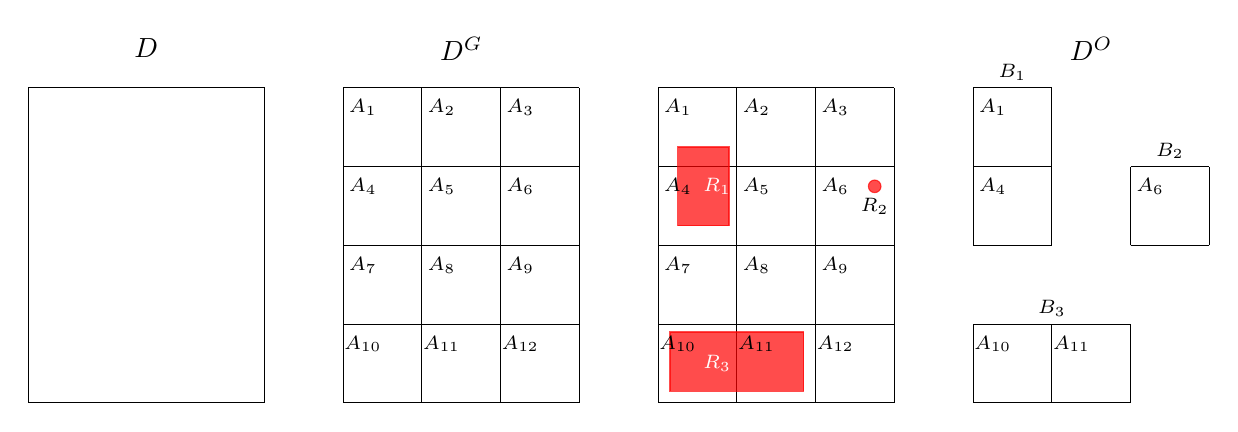
\begin{tikzpicture}
% Continuous domain D
\begin{scope}[xshift = -4cm]
\node at (1.5,4.5) {$D$};
\draw (0, 0) rectangle (3, 4);% node [below left] {$D$};
\end{scope}
% Discretised domain, D^G
\node at (1.5,4.5) {$D^G$};
\draw[step=1cm] (0,0) grid (3,4);
\node at (0.25,3.75) {\scriptsize $A_1$};
\node at (1.25,3.75) {\scriptsize $A_2$};
\node at (2.25,3.75) {\scriptsize $A_3$};
\node at (0.25,2.75) {\scriptsize $A_4$};
\node at (1.25,2.75) {\scriptsize $A_5$};
\node at (2.25,2.75) {\scriptsize $A_6$};
\node at (0.25,1.75) {\scriptsize $A_7$};
\node at (1.25,1.75) {\scriptsize $A_8$};
\node at (2.25,1.75) {\scriptsize $A_9$};
\node at (0.25,0.75) {\scriptsize $A_{10}$};
\node at (1.25,0.75) {\scriptsize $A_{11}$};
\node at (2.25,0.75) {\scriptsize $A_{12}$};
% Discretised domain, D^G, with observations
\begin{scope}[xshift = 4cm]
\draw[step=1cm] (0,0) grid (3,4);
\filldraw[color=red, fill=red, opacity = 0.7] (0.25, 3.25) rectangle (0.9, 2.25);
\node at (0.75,2.75) {\scriptsize \textcolor{white}{$R_1$}};
\filldraw[color=red, fill=red, opacity = 0.7] (0.15, 0.15) rectangle (1.85, 0.9);
\node at (0.75,0.5) {\scriptsize \textcolor{white}{$R_3$}};
\filldraw[red, opacity = 0.7] (2.75,2.75) circle (0.08cm);
\node at (2.75,2.5) {\scriptsize $R_2$};
\node at (0.25,3.75) {\scriptsize $A_1$};
\node at (1.25,3.75) {\scriptsize $A_2$};
\node at (2.25,3.75) {\scriptsize $A_3$};
\node at (0.25,2.75) {\scriptsize $A_4$};
\node at (1.25,2.75) {\scriptsize $A_5$};
\node at (2.25,2.75) {\scriptsize $A_6$};
\node at (0.25,1.75) {\scriptsize $A_7$};
\node at (1.25,1.75) {\scriptsize $A_8$};
\node at (2.25,1.75) {\scriptsize $A_9$};
\node at (0.25,0.75) {\scriptsize $A_{10}$};
\node at (1.25,0.75) {\scriptsize $A_{11}$};
\node at (2.25,0.75) {\scriptsize $A_{12}$};
\end{scope}
% observation supports
\begin{scope}[xshift = 8cm]
\node at (1.5,4.5) {$D^O$};
\draw[step=1cm] (0,4) grid (1,2);
\draw[step=1cm] (0,0) grid (2,1);
\draw[step=1cm] (2,2) grid (3,3);
\node at (0.5,4.2) {\scriptsize $B_1$};
\node at (0.25,3.75) {\scriptsize $A_1$};
\node at (0.25,2.75) {\scriptsize $A_4$};
\node at (2.5,3.2) {\scriptsize $B_2$};
\node at (2.25,2.75) {\scriptsize $A_6$};
\node at (1,1.2) {\scriptsize $B_3$};
\node at (0.25,0.75) {\scriptsize $A_{10}$};
\node at (1.25,0.75) {\scriptsize $A_{11}$};

\end{scope}
\end{tikzpicture}
\caption{
An illustration of how the continuous spatial domain, $D$, is discretised into the set $D^G$ of BAUs, and how the observation domain, $D^O$, is derived from the observation supports.
(Left panel) The continuous spatial domain, $D$.
(Centre-left panel) The spatial domain discretised into $N = 12$ BAUs, $D^G \equiv \{A_i: i = 1, \dots, 12\}$.
(Centre-right panel) $D^G$ superimposed with $m = 3$ observations, two of which are areally-referenced ($R_1$ and $R_3$), and one that is point-referenced ($R_2$).  
(Right panel) 
%The observation domain, $D^O$: The observation supports that comprise $D^O$ are $B_1 \equiv A_1 \cup A_4$,  $B_2 \equiv A_6$, and $B_3 \equiv A_{10} \cup A_{11}$.
The observation domain, \mbox{$D^O \equiv \{B_j : j = 1, \dots, m\}$}, where $B_1 \equiv A_1 \cup A_4$,  $B_2 \equiv A_6$, and $B_3 \equiv A_{10} \cup A_{11}$. 
}\label{fig:BAU_intuition}
\end{figure}

Define the conditional mean of the data as $\vec{\mu}_Z \equiv \left(\E{Z_1 \mid \vec{\mu}}, \dots, \E{Z_m \mid \vec{\mu}}\right)^\tp$, where henceforth the supports of $\{Z_1, \dots, Z_m\}$ are $\{B_1, \dots, B_m\}$, respectively. 
 Since each $B_j \in D^O$ is either a BAU or a union of BAUs, one can construct an $m\times N$ matrix 
\begin{equation}\label{eqn:C_Z}
\vec{C}_Z \equiv \Big(w_{ij}\mathbb{I}(i \in c_j) : i = 1, \dots, N; j = 1, \dots, m\Big),
\end{equation} 
where $\mathbb{I}(\cdot)$ is the indicator function, such that
\begin{equation}\label{eqn:mu_Z}
\vec{\mu}_Z = \vec{C}_Z\vec{\mu}.  
\end{equation} 
 %%%%%%Note that in \pkg{FRK} v1, \cite{FRK_paper} applied $\vec{C}_Z$ directly to $\vec{Y}$: With the identity link function, implicit in \pkg{FRK} v1, $\vec{\mu}$ and $\vec{Y}$ are equivalent. 
 %%%%%% C_ZC_pAppendix
 $\vec{C}_Z$ aggregates the BAU-level mean process, $\vec{\mu}$, over the observation supports and, depending on the weights in (\ref{eqn:C_Z}), it can correspond to a weighted average or a weighted sum over the BAUs. See Appendix \ref{Appendix:Incidence matrices: Cz and Cp} for details. 
 %%%%%% C_ZC_pAppendix
%In \pkg{FRK} v2, the weights $w_{ij}$ may be controlled through the argument \mbox{\code{normalise\_wts}} and the \code{wts} field of the \class{SpatialPixelsDataFrame}/\class{SpatialPolygonsDataFrame} object \citep{Pebesma_2005_sp_package} used to store the BAUs.  
% Specifically, the \code{wts} field allows one to attribute each BAU to a \textit{relative} weight $v_i$, $i = 1, \dots, N$, such that $w_{ij} \propto v_i$, where the constant of proportionality can vary with $j$.   
% For example, if the BAUs are of unequal area, then one may wish to set $v_i = |A_i|$. 
% By default (and implicit in \pkg{FRK} v1), each $v_i$ is set to 1. 
%  The argument \mbox{\code{normalise\_wts}} controls whether $\vec{C}_Z$ corresponds to a weighted sum or a weighted average. If set to \code{FALSE}, then $w_{ij} = v_i$ for all $j$ (weighted sum); if set to \mbox{\code{TRUE}} (default and implicit in \pkg{FRK} v1), then the $\{w_{ij}\}$ are normalised so that each row of $\vec{C}_Z$ sums to 1 (weighted average) and $w_{ij} = v_i / \sum_{l \in c_j} v_l$.   
%%  Note that if $v_i = |A_i|$ and \mbox{\code{normalise\_wts = TRUE}}, the $j$th row sum of $\vec{C}_Z$ is $\sum_{i \in c_j} |A_i| = |B_j|$, so that the normalised weights are $w_{ij} = |A_i|/|B_j|$.  
%  Note that if $v_i = |A_i|$ and \mbox{\code{normalise\_wts = TRUE}}, the normalised weights are $w_{ij} = |A_i|/|B_j|$, since the BAUs are disjoint and $\sum_{i \in c_j} |A_i| = |B_j|$. 
  

 %%%%%% C_ZC_pAppendix
%Denoting the mean of $Z_j$, which is the $j$th element of $\vec{\mu}_Z$, by $\mu_{Z_j}$, we assume that 
Denoting the $j$th element of $\vec{\mu}_Z$ by $\mu_{Z_j}$, we assume that 
\begin{equation}\label{eqn:Z_j|mu(.)}
[Z_j \mid \vec{\mu}, \psi] = \text{EF}(\mu_{Z_j}, \psi); \quad j = 1, \dots, m,
\end{equation}
where EF corresponds to a probability distribution in the exponential family with dispersion parameter $\psi$ and, for generic random quantities $A$ and $B$, $[A \mid B]$ denotes the probability distribution of $A$ given $B$. 
 We assume that $\psi$ is spatially invariant; with the parameterisations assumed by \pkg{FRK} v2, $\psi = 1$ for some distributions in the exponential family (e.g., the binomial, negative-binomial, and Poisson distributions).

Together, (\ref{eqn:mu_Z}) and (\ref{eqn:Z_j|mu(.)}) imply that a given observation depends only on the value of the mean process at the corresponding observation support, rather than on means elsewhere in the domain. 
Further, we assume that all observations are conditionally independent given the latent spatial process and that they are all from the same exponential family member: Specifically, 
\[
[\vec{Z} \mid \vec{\mu}_Z, \psi] = \prod_{j=1}^m \text{EF}(\mu_{Zj}, \psi).
\]
As we only consider data models in the exponential family, $\ln{[\vec{Z}  \mid  \vec{\mu}_Z, \psi]}$ may be written as  
\begin{equation}\label{eqn:ln[Z|Y],ExpFam}
\ln{[\vec{Z} \mid \vec{\mu}_Z, \psi]}
=
\sum_{j=1}^m\left\{
\frac{Z_j\lambda(\mu_{Z_j}) - b(\lambda(\mu_{Z_j}))}{a(\psi)} + c(Z_j, \psi)\right\},
\end{equation}
where $a(\cdot)$, $b(\cdot)$, and $c(\cdot, \cdot)$ are deterministic functions specific to the chosen exponential family member, and $\lambda(\cdot)$ is the canonical parameter.


The model employed by \pkg{FRK} v2 can be summarised as follows. 
\begin{gather}
    Z_j \mid \mu_{Z_j}, \psi \inddist \text{EF}(\mu_{Z_j}, \psi); \quad j = 1, \dots, m, \label{eqn:new_model_Z}\\
    \vec{\mu}_Z = \vec{C}_Z \vec{\mu}, \label{eqn:new_model_muZ}\\
    g(\vec{\mu}) = \vec{Y}, \label{eqn:new_model_g(mu)}\\
    \vec{Y} = \vec{T} \vec{\alpha} + \vec{S} \vec{\eta} + \vec{\xi}, \label{eqn:new_model_Y}\\
    \vec{\eta} \mid \vec{\vartheta} \sim \Gau(\vec{0}, \vec{Q}^{-1}), \\
    \vec{\xi} \mid \sigma^2_\xi \sim \Gau(\vec{0}, \sigma^2_\xi \vec{V}), \label{eqn:new_model_priors}
\end{gather}
 where $\vec{V}$ is a known, positive-definite diagonal matrix which, in the absence of problem specific fine-scale information, can simply be set to $\vec{I}$, and $\sigma^2_\xi$ is either unknown and estimated or it is possible for the user to provide it.  
 In a spatio-temporal setting, a more complex model for $\vec{\xi}$ is allowed; see Section \ref{sec:spatio-temporal}. 
 Note that \pkg{FRK} v2 is backwards compatible, since an identity link function and a Gaussian data model in (\ref{eqn:new_model_Z}) yields the model used in \pkg{FRK} v1; then $\psi$ is simply the measurement-error variance $\sigma^2_\epsilon$ in $Z_j \mid \mu_{Z_j}, \sigma^2_\epsilon \sim \Gau(\mu_{Z_j}, \sigma^2_\epsilon)$. 



\subsection{Estimation}\label{subsection:02-03:Estimation}

We now derive the likelihood functions required for model fitting, outline the intractable integrals that arise when non-Gaussian data models are fitted, and describe how \pkg{TMB} \citep{Kristensen_2016_TMB} is used to obtain estimates of the parameters/fixed effects and predictions of the random effects.


%\subsubsection{Complete-data likelihood}

Noting that $\vec{\mu}_Z$ is, through (\ref{eqn:new_model_muZ})--(\ref{eqn:new_model_Y}), completely determined by $\vec{\alpha}$, $\vec{\eta}$, and $\vec{\xi}$,  
 the complete-data likelihood function for our model is
\begin{equation}\label{eqn:04:Joint_Likelihood}
    L(\vec{\theta}; \vec{Z}, \vec{\eta}, \vec{\xi})
    \equiv 
    [\vec{Z}, \vec{\eta}, \vec{\xi} \mid \vec{\theta}]
    =
    [\vec{Z} \mid \vec{\mu}_Z, \psi]
    [\vec{\eta} \mid \vec{\vartheta}]
    [\vec{\xi} \mid \sigma^2_\xi], 
\end{equation}
 where $
 \vec{\theta}
 \equiv
 (
 \vec{\alpha}^\tp,
 \vec{\vartheta}^\tp, 
 \sigma^2_\xi, 
 \psi
 )^\tp$, and $\vec{\vartheta}$ denotes the variance-covariance components associated with either $\vec{K}$ or $\vec{Q}$.
The complete-data log-likelihood function, $l(\vec{\theta}; \vec{Z}, \vec{\eta}, \vec{\xi})$, is simply the logarithm of (\ref{eqn:04:Joint_Likelihood}). %, 
%\begin{equation}\label{eqn:04:Joint_Log_Likelihood}
%    l(\vec{\theta}; \vec{Z}, \vec{\eta}, \vec{\xi}) 
%    \equiv 
%    \ln{L(\vec{\theta}; \vec{Z}, \vec{\eta}, \vec{\xi})}
%    =
%    \ln{[\vec{Z} \mid \vec{\mu}_Z, \psi]}
%    +
%    \ln{[\vec{\eta} \mid \vec{\vartheta}]}
%    +
%    \ln{[\vec{\xi} \mid \sigma^2_\xi]}.
%\end{equation}
Under the modelling assumptions (\ref{eqn:new_model_Z})--(\ref{eqn:new_model_priors}), the conditional density functions  $[\vec{\eta}\mid\vec{\vartheta}]$ and $[\vec{\xi} \mid \sigma^2_\xi]$ are invariant to the specified link function and the assumed distribution of the response variable. 
 Of course, this invariance does not hold for $[\vec{Z} \mid \vec{\mu}_Z, \psi]$. %; see (\ref{eqn:ln[Z|Y],ExpFam}). 


%\subsubsection{observed-data likelihood}\label{sec:marginal_likelihood}

The observed-data likelihood, which depends on the observations $\vec{Z}$ and not on the unobserved random effects $\vec{u} \equiv (\vec{\eta}^\tp, \vec{\xi}^\tp)^\tp$, is given by integrating out $\vec{u}$ from (\ref{eqn:04:Joint_Likelihood}):
\begin{equation}\label{eqn:02-04:LikelihoodTheta}
    L^*(\vec{\theta}; \vec{Z}) 
    \equiv
    \int_{\mathbb{R}^{{p}}}
    L(\vec{\theta} ; \vec{Z}, \vec{u}) \d \vec{u}, 
%    =
%    \int_{\mathbb{R}^{{p}}}
%    \exp\left\{l(\vec{\theta} ; \vec{Z}, \vec{u})\right\} \d \vec{u},
\end{equation}
where ${p}$ is the total number of random effects in the model. 
 The observed-data log-likelihood function is $l^*(\vec{\theta}; \vec{Z}) \equiv \log{L^*(\vec{\theta}; \vec{Z})}$. 
When the data are non-Gaussian, the integral in (\ref{eqn:02-04:LikelihoodTheta}) is typically intractable and must be approximated. 
In \pkg{FRK} v2, a Laplace approximation is used, which we now briefly describe. 


Let $\hat{\vec{u}}\equiv\hat{\vec{u}}(\vec{\theta}, \vec{Z})$ be a mode of $l(\vec{\theta}; \vec{Z}, \vec{u})$ with respect to $\vec{u}$, 
% \begin{equation*}
% \left.\nabla_{\vec{u}} l(\vec{\theta} ; \vec{Z}, \vec{u})\right\rvert_{\vec{u}=\hat{\vec{u}}} = \vec{0},
% \end{equation*}
 and let %$\vec{H}$ be the negative of the inverse Hessian matrix of $l(\vec{\theta} ; \vec{Z}, \vec{u})$ with respect to $\vec{u}$, evaluated at $\hat{\vec{u}}$:
\begin{equation*}
    \vec{H} 
    \equiv
    -\left(\left.\nabla_{\vec{u}} \nabla_{\vec{u}} l(\vec{\theta} ; \vec{Z}, \vec{u}) \right\rvert_{\vec{u}=\hat{\vec{u}}}\right)^{-1},
\end{equation*}
 where $\nabla_{\vec{u}}$ denotes the gradient with respect to $\vec{u}$. 
 A second-order Taylor-series approximation of $l(\vec{\theta} ; \vec{Z}, \vec{u})$ about $\vec{u} =  \hat{\vec{u}}$ results in an approximation of (\ref{eqn:04:Joint_Likelihood}) that has the form of an un-normalised Gaussian density in terms of $\vec{u}$, with mean vector $\hat{\vec{u}}$ and covariance matrix $\vec{H}$. 
 Substitution of this approximation into (\ref{eqn:02-04:LikelihoodTheta}) and evaluation of the integral, yields the Laplace approximation of the observed-data likelihood, $L^*(\vec{\theta}; \vec{Z})
    \approx L(\vec{\theta} ; \vec{Z}, \hat{\vec{u}})
    (2\pi)^{\frac{{p}}{2}}\left|\vec{H}\right|^{\frac{1}{2}}$.
% This allows $\vec{u}$ to be integrated out of $L(\vec{\theta}; \vec{Z}, \vec{u})$, yielding the Laplace approximation of the observed-data log likelihood, $l^*(\vec{\theta}; \vec{Z}) \approx l(\vec{\theta} ;  \vec{Z}, \hat{\vec{u}}) + \frac{{p}}{2} \ln{2\pi} + \frac{1}{2} \ln{\left|\vec{H}\right|}$.
 
 
 Note that $[\vec{u} \mid \vec{Z}, \vec{\theta}] \propto [\vec{u}, \vec{Z} \mid \vec{\theta}]$, which is equal to the complete-data likelihood function, $L(\vec{\theta}; \vec{Z}, \vec{u})$. 
 Therefore, since the Laplace approximation replaces $L(\vec{\theta}; \vec{Z}, \vec{u})$ with a term that has the form of an un-normalised Gaussian density in terms of $\vec{u}$, it follows that, approximately, $\vec{u} \mid \vec{Z}, \vec{\theta} \sim \Gau(\hat{\vec{u}}, \vec{H})$. 
  In the software we use (\pkg{TMB}; see below), estimates of $\hat{\vec{u}}$ and $\vec{H}^{-1}$ are provided, which makes prediction of $\vec{u}$ and any function of it straightforward via the predictive distribution and its MC simulation (see Section \ref{subsection:Prediction}). 



%%%%%%%%%%%% LONGER VERSION
 

% Let $\vec{u} \equiv (\vec{\eta}^\tp, \vec{\xi}^\tp)^\tp \in \mathbb{R}^{{p}}$ denote the random effects in our model, where ${p}$ is the total number of random effects.
% The observed-data likelihood function, $L^*(\vec{\theta}; \vec{Z})$, is obtained by integrating out the random effects from the complete-data likelihood function;
% \begin{equation}\label{eqn:02-04:LikelihoodTheta}
%     L^*(\vec{\theta}; \vec{Z}) 
%     = 
%     \int_{\mathbb{R}^{{p}}}
%     L(\vec{\theta} ; \vec{Z}, \vec{u}) \d \vec{u} 
%     \equiv 
%     \int_{\mathbb{R}^{{p}}}
%     \exp\left\{l(\vec{\theta} ; \vec{Z}, \vec{u})\right\} \d \vec{u}.
% \end{equation}
%  When the data model is non-Gaussian, this integral is intractable and requires either numerical or analytical approximation.
%  The Laplace approximation involves approximating $ L(\vec{\theta} ; \vec{Z}, \vec{u})$ with a Gaussian distribution centred at a mode of $ L(\vec{\theta} ; \vec{Z}, \vec{u})$.
% Define $\hat{\vec{u}}\equiv\hat{\vec{u}}(\vec{\theta}, \vec{Z})$ to be a mode of $l(\vec{\theta}; \vec{Z}, \vec{u})$ with respect to $\vec{u}$.
%  \begin{equation*}
%  \left.\nabla_{\vec{u}} l(\vec{\theta} ; \vec{Z}, \vec{u})\right\rvert_{\vec{u}=\hat{\vec{u}}} = \vec{0},
%  \end{equation*}
%  where $\nabla_{\vec{u}}$ denotes the gradient with respect to $\vec{u}$.
% A second-order Taylor series approximation of $l(\vec{\theta} ; \vec{Z}, \vec{u})$ about $\hat{\vec{u}}$ yields
% \begin{equation}\label{eqn:02-04:TaylorApprox}
% l(\vec{\theta} ; \vec{Z}, \vec{u}) 
%     \approx 
%     l(\vec{\theta} ; \vec{Z}, \hat{\vec{u}}) 
%     -
%     \frac{1}{2}(\vec{u} - \hat{\vec{u}})^\tp \vec{H}^{-1}(\vec{u} - \hat{\vec{u}}), 
% \end{equation}
% where 
%  the first-order term is zero as we have expanded about a stationary point, and 
% $\vec{H}$ is the negative of the inverse Hessian matrix of $l(\vec{\theta} ; \vec{Z}, \vec{u})$ with respect to $\vec{u}$ at $\hat{\vec{u}}$:
% \begin{equation*}
%     \vec{H} = \vec{H}(\vec{\theta}; \vec{Z})
%     =
%     -\left(\left.\nabla_{\vec{u}} \nabla_{\vec{u}} l(\vec{\theta} ; \vec{Z}, \vec{u}) \right\rvert_{\vec{u}=\hat{\vec{u}}}\right)^{-1}.
% \end{equation*}
% Exponentiating (\ref{eqn:02-04:TaylorApprox}), we have that
% \begin{equation}\label{eqn:approx_joint_likelihood}
%     L(\vec{\theta} ; \vec{Z}, \vec{u}) 
%     \approx 
%     L(\vec{\theta} ; \vec{Z}, \hat{\vec{u}}) \exp\left\{
%     -
%     \frac{1}{2}(\vec{u} - \hat{\vec{u}})^\tp \vec{H}^{-1}(\vec{u} - \hat{\vec{u}})
%     \right\},
% \end{equation}
% while substituting (\ref{eqn:approx_joint_likelihood}) into the observed-data likelihood (\ref{eqn:02-04:LikelihoodTheta}) yields the Laplace approximation of the observed-data likelihood:
% \begin{align*}
%     L^*(\vec{\theta}; \vec{Z})
%      &= \int_{\mathbb{R}^{{p}}} L(\vec{\theta} ; \vec{Z}, \vec{u}) \d \vec{u}\\
%      &= \int_{\mathbb{R}^{{p}}} \exp\left\{l(\vec{\theta} ; \vec{Z}, \vec{u})\right\} \d \vec{u}\\
%     &\approx \int_{\mathbb{R}^{{p}}} L(\vec{\theta} ; \vec{Z}, \hat{\vec{u}}) \exp\left\{
%     -
%     \frac{1}{2}(\vec{u} - \hat{\vec{u}})^\tp \vec{H}^{-1}(\vec{u} - \hat{\vec{u}})
%     \right\} \d \vec{u}\\
%      &= L(\vec{\theta} ; \vec{Z}, \hat{\vec{u}})\int_{\mathbb{R}^{{p}}} \exp\left\{-\frac{1}{2}(\vec{u} - \hat{\vec{u}})^\tp \vec{H}^{-1} (\vec{u} - \hat{\vec{u}})\right\} \d \vec{u}\\
%      &= L(\vec{\theta} ; \vec{Z}, \hat{\vec{u}})
%      \left|2\pi\vec{H}\right|^{\frac{1}{2}}\\
%     &= L(\vec{\theta} ; \vec{Z}, \hat{\vec{u}})
%     (2\pi)^{\frac{{p}}{2}}\left|\vec{H}\right|^{\frac{1}{2}}.
% \end{align*}
%  Hence, the Laplace approximation of the observed-data likelihood is
%  \begin{equation}\label{eqn:02-04:marglike}
%      L^*(\vec{\theta}; \vec{Z})
%      \approx
%      L(\vec{\theta} ; \hat{\vec{u}}, \vec{Z})
%      (2\pi)^{\frac{s}{2}}\left|\vec{H}\right|^{\frac{1}{2}}.
%  \end{equation}
% The Laplace approximation of the observed-data log-likelihood is then
% \begin{equation}\label{eqn:02-04:margloglike}
% l^*(\vec{\theta}; \vec{Z}) = 
%     \ln{L^*(\vec{\theta}; \vec{Z})}
%     \approx
%     l(\vec{\theta} ;  \vec{Z}, \hat{\vec{u}}) + \frac{{p}}{2} \log{2\pi} + \frac{1}{2} \log{\left|\vec{H}\right|}.
% \end{equation}
%
%% % The reason for $\hat{\vec{u}}$ needing to be a mode (rather than the weaker condition of it being a stationary point) is apparent: in order for the Gaussian density function used to derive the approximation to be well defined (and integrate to one), its variance-covariance matrix must be positive definite, which implies that $\hat{\vec{u}}$ must be a maximum (i.e., a mode of the log-likelihood function). 
%
%% % As an aside, a maximum likelihood estimate of the parameters derived from (\ref{eqn:02-04:margloglike}) is the maximum of the function $L^*(\vec{\theta}; \vec{Z})$ with respect to the parameters $\vec{\theta}$; it is, in general, \textit{not} the maximum of $L(\vec{\theta}; \vec{Z}, \vec{u})$. This is a subtle yet important distinction; see Figure \ref{fig:02-04:TwoProbMass} for further clarification.  
%
% The Laplace approximation implicitly assumes the posterior distribution of the random effects is Gaussian.  
%  we may express the complete-data  likelihood function as
%  \begin{align*}
%      L(\vec{\theta}; \vec{Z}, \vec{u})
%      &= 
%      [\vec{Z}, \vec{u} \mid \vec{\theta}]
%      =
%      [\vec{u} \mid \vec{Z}, \vec{\theta}][\vec{Z} \mid \vec{\theta}],
%  \end{align*}
% To see this, substituting the complete-data likelihood function with its Laplace approximation, we have that
% \begin{align*}
%     [\vec{u} \mid \vec{Z}, \vec{\theta}]
%     &=
%     \frac{L(\vec{\theta}; \vec{Z}, \vec{u})}{[\vec{Z} \mid \vec{\theta}]}\\
%     &\approx 
%     \frac{L(\vec{\theta} ; \vec{Z}, \hat{\vec{u}}) }{[\vec{Z} \mid \vec{\theta}]}\exp\left\{
%     -
%     \frac{1}{2}(\vec{u} - \hat{\vec{u}})^\tp \vec{H}^{-1}(\vec{u} - \hat{\vec{u}})
%     \right\}\\
%     &\propto
%     \exp\left\{
%     -
%     \frac{1}{2}(\vec{u} - \hat{\vec{u}})^\tp \vec{H}^{-1}(\vec{u} - \hat{\vec{u}})
%     \right\},
% \end{align*}
% so that (approximately) $\vec{u} \mid \vec{Z}, \vec{\theta} \sim \Gau(\hat{\vec{u}}, \vec{H})$.
%

\subsubsection[Model fitting with TMB]{Model fitting with \pkg{TMB}}

\pkg{FRK} v2 supplies the \proglang{R} package \pkg{TMB} \citep{Kristensen_2016_TMB} with a \proglang{C++} template function that defines $l(\vec{\theta} ; \vec{Z}, \vec{u})$. \pkg{TMB} then computes the Laplace approximation of the observed-data log-likelihood, $l^*(\vec{\theta}; \vec{Z})$, and it automatically computes its derivatives; these quantities are then invoked via a user-defined optimising function (\fct{nlminb} is used by default). 
 \pkg{TMB} uses \pkg{CppAD} \citep{CppAD_Package} for automatic differentiation, and it uses the linear-algebra libraries \pkg{Eigen} \citep{Eigen} and \pkg{Matrix} \citep{Matrix_Package} for vector and matrix operations in \proglang{C++} and \proglang{R}, respectively. 
 Use of these packages yields high computational efficiency. 
\pkg{TMB}'s implementation of automatic differentiation is a key reason why \pkg{FRK} v2 can easily cater for a large variety of response distributions and link functions, as each response-distribution/link-function combination does not need to be considered on a case-by-case basis.

Note that all unknown quantities are treated as random in \pkg{TMB} (with a flat prior assumed if a prior is not provided).
 To retain \pkg{FRK} v1's mixed-model interpretation, we fix the model parameters and fixed effects to their posterior-mode estimates and then treat them as non-random quantities.
%We fix the parameters to their posterior-mode estimates and then treat them as non-random quantities when doing prediction; however, we let the user decide if the fixed effects $\vec{\alpha}$ are treated as fixed or random. 
%If they fixed, flagged by setting \code{kriging = "simple"} in the function \fct{predict}, they are treated in the same way as the parameters. 
%If they are random, we jointly sample $\vec{\alpha}$ along with the random effects $\vec{u}$ in the prediction stage;  this choice accounts for the uncertainty in estimation of $\vec{\alpha}$, and so it is flagged by setting \code{kriging = "universal"} (see Cressie (1993, Ch. 3) OR AN EARLIER REFERENCE THAT IS IN THAT CHAPTER for the equivalence of using a flat prior on $\vec{\alpha}$ to performing universal kriging). 


%%%%% Notes which are useful to keep, but do not need to be in the paper (could put them in the thesis chapter):

%The justification for fixing the parameters/fixed-effects to their mode estimators is as follows. 
%\pkg{TMB} uses the Laplace approximation, and so implicitly assumes that
%\begin{equation}
%    \begin{bmatrix}
%    \vec{\theta} \\
%    \vec{u}
%    \end{bmatrix}
%    \sim \Gau\left( 
%    \begin{bmatrix}
%    \hat{\vec{\theta}} \\
%    \hat{\vec{u}}
%    \end{bmatrix}, 
%    \begin{bmatrix}
%    \vec{Q}_{\theta, \theta} & \vec{Q}_{\theta, u} \\
%    \vec{Q}_{u, \theta} & \vec{Q}_{u, u}
%    \end{bmatrix}^{-1}
%    \right).
%\end{equation}
%If we fix $\vec{\theta}$ to their mode estimates, that is, if we condition on $\vec{\theta} = \hat{\vec{\theta}}$, then,
%by well known properties of the Gaussian distribution \citep[e.g., ][App. A]{RW_2006_Gaussian_Processes_for_Machine_Learning}, we have that 
%$\ENoLR{\vec{u} \mid \vec{\theta} = \hat{\vec{\theta}}} = \hat{\vec{u}}$
%and
%$\precisionNoLR{\vec{u} \mid \vec{\theta} =  \hat{\vec{\theta}}} = \vec{Q}_{u, u}$.


\subsection{Prediction and uncertainty quantification}\label{subsection:Prediction}


We now discuss spatial prediction and uncertainty quantification of the predictions. 
There are three principal quantities that could be of interest to the user, namely the latent process 
%$Y(\cdot)$ and mean process $\mu(\cdot)$ in (\ref{eqn:mu_linked_to_Y}), and data at unobserved locations. 
$\vec{Y}$ and mean process $\vec{\mu}$ in (\ref{eqn:new_model_g(mu)}), and data at unobserved locations. 
% To produce predictions and associated uncertainties, we need to determine the posterior distribution of these quantities.
%For each quantity, we use the posterior expectation as our predictor. % ; a decision theoretic justification for this choice is provided by \citet*[ch.~3]{Cressie_1993_stats_for_spatial_data}.
Recall that the Laplace approximation implies that the conditional distribution of $\vec{u} \equiv (\vec{\eta}^\tp, \vec{\xi}^\tp)^\tp$ is, approximately, $\vec{u} \mid \vec{Z}, \vec{\theta} \sim \Gau(\hat{\vec{u}}, \vec{H})$; since $\vec{Y}$ is a linear function of $\vec{u}$, approximate inference on $\vec{Y}$ can be carried out using well-known formulas. 
%  However, the posterior distribution of a non-linear function of $Y(\cdot)$ (e.g., the mean $\mu(\cdot)$ in (\ref{eqn:mu_linked_to_Y})) is typically not available in closed form, and some approximation is required.
  However, the posterior distribution of a non-linear function of $\vec{Y}$ (e.g., the mean $\vec{\mu}$ in (\ref{eqn:new_model_g(mu)})) is typically not available in closed form, and some approximation is required.
%  In \pkg{FRK} v2, we use a Monte Carlo (MC) approach to inference on $\vec{u} \equiv (\vec{\eta}^\tp, \vec{\xi}^\tp)^\tp$.
 In \pkg{FRK} v2, we therefore use a Monte Carlo (MC) approach to inference on non-linear functions of $\vec{Y}$, by first drawing a sample from the approximate conditional distribution of $\vec{u}$ and then transforming the sample accordingly. 
  


 Recall that $\vec{Y} = \vec{T}\vec{\alpha} + \vec{S}\vec{\eta} + \vec{\xi}$, which can be rewritten as $\vec{Y} = \vec{T}\vec{\alpha} + [\vec{S} \; \vec{I}] \,\vec{u}$. 
 We thus define $\vec{Y}_{\!\text{MC}}$, an $N \times n_{\text{MC}}$ matrix whose columns are the $n_{\text{MC}}$ MC samples from $[\vec{Y} \mid \vec{Z}, \vec{\theta}]$, as 
\begin{equation}\label{eqn:Y_MC_simple}
\vec{Y}_{\!\text{MC}}
\equiv \vec{T}\hatt{\vec{A}}[A] + [\vec{S} \; \vec{I}] \,\vec{U},
\end{equation}
where each of the $n_{\text{MC}}$ columns of the matrix $\hatt{\vec{A}}[A]$ is the estimate of $\vec{\alpha}$, and each of the $n_{\text{MC}}$ columns of the matrix $\vec{U}$ is a draw from $\vec{u} \mid \vec{Z}, \vec{\theta} \sim \Gau(\hat{\vec{u}}, \vec{H})$.  
 We obtain MC samples of the $N$-dimensional vector $\vec{\mu}$ from $[\vec{\mu} \mid \vec{Z}, \vec{\theta}]$ via the $N\times n_{MC}$ matrix $\vec{M} \equiv g^{-1}(\vec{Y}_{\!\text{MC}})$, where $g^{-1}(\cdot)$ is applied element-wise. 
  Not only does \pkg{FRK} v2 predict $\vec{\mu}$, it also allows prediction of data over all $N$ BAUs, which we write as $\vec{Z}^* \equiv (Z^*_1, \dots, Z^*_N)^\tp$. 
  We assume that these data are from the same exponential family model as that of the original data, $\vec{Z}$. 
 MC samples of $\vec{Z}^*$ can then be constructed straightforwardly using $\vec{M}$. 
 Note that \pkg{FRK} v2 provides the user with $\vec{M}$ which, if needed, could be used to predict data with link function $g(\cdot)$ but from a distribution that is different from that of the original data.


For each quantity, we use the posterior expectation as the predictor, which can be estimated by simply taking row-wise averages of the matrices of samples defined above. 
In a Gaussian setting, a commonly used metric for uncertainty quantification is the root-mean-squared prediction error (RMSPE). 
In a non-Gaussian setting, it can be difficult to interpret the RMSPE, and it is often more intuitive to quantify uncertainty through the width of the prediction intervals. Hence, in \pkg{FRK} v2, we also use the MC sampling approach described above to compute user-specified percentiles of the predictive distribution.  


%% NB: A longer form of the prediction section, which also discusses analytic solutions, is commented out in the appendices

%%The MSPE has an appealing form when the conditional expectation, $\E{A \mid \vec{Z}}$, is used as a predictor of some quantity $A$; specifically, using the law of total expectation, and the definition of conditional variance, it can be shown that
%%% \begin{align}\label{eqn:04-03:GeneralMSPE}
%%%     \MSPEtwoarg{\E{A \mid \vec{Z}}}{A}
%%%     &\equiv
%%%     \ESquare{\left\{\E{A \mid \vec{Z}}-A\right\}^2} \nonumber \\
%%%     &=
%%%     \ESquare{\E{\left\{\E{A \mid \vec{Z}}-A\right\}^2 \mathrel{\Big|} \vec{Z}}} \nonumber \\
%%%     &=
%%%     \ESquare{\var{A \mid \vec{Z}}}.
%%%     %= \var{A} - \varCurly{\E{A \mid \vec{Z}}},
%%% \end{align}
%%\begin{equation}\label{eqn:04-03:GeneralMSPE}
%%    \MSPEtwoarg{\E{A \mid \vec{Z}}}{A}
%%    \equiv
%%    \ESquare{\left\{\E{A \mid \vec{Z}}-A\right\}^2} 
%%    % =
%%    % \ESquare{\E{\left\{\E{A \mid \vec{Z}}-A\right\}^2 \mathrel{\Big|} \vec{Z}}}
%%    =
%%    \ECurly{\var{A \mid \vec{Z}}},
%%\end{equation}
%%where $\MSPEtwoarg{\cdot}{\cdot}$ is a function of two arguments (the predictor, and the predictand). 
%%If $A$ and $\vec{Z}$ are both Gaussian, then $A \mid \vec{Z}$ exhibits a feature known as conditional homoskedasticity; that is, the conditional variance $\var{A \mid \vec{Z}}$ \textit{does not} depend on $\vec{Z}$ \citep[e.g., ][p.~110]{Cressie_1993_stats_for_spatial_data}. 
%%In this case, (\ref{eqn:04-03:GeneralMSPE}) is equal to  $\var{A \mid \vec{Z}}$. 
%%When the conditional variance \textit{does} depend on $\vec{Z}$, (\ref{eqn:04-03:GeneralMSPE}) can be estimated by dropping the expectation. 
%% Then the MSPE (\ref{eqn:04-03:GeneralMSPE}) is given by
%% \begin{equation}\label{eqn:04-03:MSPEyGivenz2}
%%     \MSPEtwoarg{\pYgivenZ{\vec{s}_0}}{Y(\vec{s}_0)} 
%%     \approx 
%%     \varCurly{Y(\vec{s}_0) \mid \vec{Z}, \vec{\theta}},
%% \end{equation}
%% where approximate equality is replaced by equality in the case of Gaussian data. 


%%%% Giving a symbol to the predictors:

%\begin{equation}\label{eqn:02-03:pYgivenZ}
%    \pYgivenZ{A_i}
%    \equiv
%    \ECurly{Y_i \mid \vec{Z}, \vec{\theta}}.
%\end{equation}
%\begin{equation}\label{eqn:04-03:muOptimalPredictor}
%    \pmugivenZ{A_i} 
%    \equiv 
%    \ECurly{\mu_i \mid \vec{Z}, \vec{\theta}} = \ECurly{g^{-1}(Y_i) \mid \vec{Z}, \vec{\theta}}.
%\end{equation}
%\begin{equation}\label{eqn:04-03:ZOptimalPredictor}
%    \hat{p}_{Z_i|\vec{Z}}
%    \equiv 
%    \ECurly{Z_i \mid \vec{Z}, \vec{\theta}},
%\end{equation}
%which, using the law of total expectation, can be shown to be equivalent to (\ref{eqn:04-03:muOptimalPredictor}). 


%%%% Computational details for sampling from u | Z, \theta:

%Denote the posterior mode and precision matrix of the random effects by $\hat{\vec{u}}$ and $\vec{Q}_{u}$, respectively. These quantities are estimated using \pkg{TMB}. 
%Define a permuted version of the precision matrix as $\vec{A} \equiv \vec{P}^\tp \vec{Q}_{u} \vec{P}$, where $\vec{P}$ is a permutation matrix. Define the upper Cholesky factor of $\vec{A}$ as $\vec{U}_P$, which is the upper triangular matrix satisfying $\vec{A} = \vec{U}_P^\tp \vec{U}_P$. Then, we have that $\vec{Q}_{u} = \vec{M}^\tp \vec{M}$, where $\vec{M} = \vec{U}_P \vec{P}^\tp$ is \textit{not} triangular.
%Now consider the usual method of transforming a standard Gaussian vector to a Gaussian vector with precision matrix $\vec{Q}_{u}$. 
%First, let $\vec{z} \sim \Gau(\vec{0}, \vec{I})$ denote a standard Gaussian random vector. Then, we have that the variance of the transformed vector $\tilde{\vec{u}} \equiv \vec{M}^{-1}\vec{z} $ is
%\begin{align*}
%    \var{\tilde{\vec{u}}}
%    = \var{\vec{M}^{-1}\vec{z}}
%    = \vec{M}^{-1}\vec{M}^{-\tp}
%    = (\vec{M}^{\tp}\vec{M})^{-1}
%    = \vec{Q}_{u}^{-1},
%\end{align*}
%as required. Note, however, that although $\vec{M}$ is sparse, it is not triangular.
%However, we have that $\vec{M}^{-1} = \vec{P} \vec{U}_P^{-1}$,
%and so $\tilde{\vec{u}}$ may equivalently be written as
%$\tilde{\vec{u}} = \vec{P} \vec{U}_P^{-1}\vec{z}$.
%Therefore, we can first solve the upper triangular system $\vec{U}_P \vec{x} = \vec{z}$, and then left-multiply $\vec{x}$ by the permutation matrix $\vec{P}$ to obtain $\tilde{\vec{u}} = \vec{P} \vec{x} = \vec{P} \vec{U}_P^{-1}\vec{z} = \vec{M}^{-1}\vec{z}$, as required. 
%This approach to generating samples fully exploits both the reduction of fill-in from matrix reordering, as well as a computationally efficient backward-solve.


%%%% Construction of Y_MC considering both kriging = simple and kriging = false

% If \code{kriging = "simple"} we construct $\vec{Y}_{\!\text{MC}}$ via 
%\begin{equation}\label{eqn:Y_MC_simple}
%\vec{Y}_{\!\text{MC}}
%\equiv \vec{T}\vec{A} + [\vec{S} \; \vec{I}] \,\vec{U},
%\end{equation}
%where $\vec{A}$ is a $q \times n_{\text{MC}}$ matrix whose columns consist of the estimated posterior mode of $\vec{\alpha}$ (and where $q$ denotes the dimension of $\vec{\alpha}$), and $\vec{U}$ is a $p \times n_{\text{MC}}$ matrix whose columns are MC samples of $\vec{u} \mid \vec{Z}, \vec{\theta}$. 
% If \code{kriging = "universal"}, then $\vec{\alpha}$ are treated as random effects and included in $\vec{u}$, and (\ref{eqn:Y_MC_simple}) is rewritten as
% \begin{equation}\label{eqn:Y_MC_universal}
%\vec{Y}_{\!\text{MC}}
%\equiv [\vec{T} \; \vec{S} \; \vec{I}] \,\vec{U},
%\end{equation}
%where $\vec{U}$ is now a $(p + q) \times n_{\text{MC}}$ matrix and includes samples of $\vec{\alpha} \mid \vec{Z}, \vec{\theta}$. 



\subsubsection{Arbitrary prediction regions}


 Often, one does not wish to predict over single BAUs but over regions spanning multiple BAUs, $\{\tilde{R}_l$, $l = 1, \dots, N_P\}$, where $N_P$ is the number of prediction regions. 
 These regions may overlap and may not coincide with entire BAUs: Our criterion for determining whether a prediction region contains a particular BAU is the same as that used for the spatial supports originally associated with the observations (see Section \ref{subsection:DataLayer}). 
 That is, we write the indices of the BAUs associated with $\tilde{R}_l$ as $\tilde{c}_l \equiv \{i : A_i \cap \tilde{R}_l \neq \emptyset\}$, for $l = 1, \dots, N_P$.
 We then define the set of prediction regions in terms of BAUs as $D^P \equiv \{\tilde{B}_l : l = 1, \dots, N_P\}$, where $\tilde{B}_l \equiv \cup_{i\in \tilde{c}_l} A_i$ is the package's representation of $\tilde{R}_l$ in terms of BAUs. %, and where $\tilde{c}_l$ is a non-empty subset of $\{1, \dots, N\}$ that gives the indices of the BAUs associated with the $k$th user-specified region, $\tilde{R}_l$.
%Here, $N_P$ is the number of areas at which spatial prediction takes place, and is equal to $|D^P|$.


%Prediction over $D^P$ requires some form of aggregation across the associated BAUs. 
%Since aggregation must be done on the response scale, we restrict prediction over arbitrary regions to the mean process and the data.  
% Let $\vec{\mu}_P \equiv \{\mu(\tilde{B}_l) : l = 1, \dots, N_P\}$ be the mean process evaluated over the prediction regions. Just as $\vec{\mu}_Z$ was constructed from the BAU-level mean process $\vec{\mu}$ via the matrix $\vec{C}_Z$ given by (\ref{eqn:C_Z}), since each $\tilde{B}_l$ is a BAU or a union of BAUs, one can construct an $N_P \times N$ matrix 
%\[
%\vec{C}_P \equiv \left(\tilde{w}_{ik}\mathbb{I}(i \in \tilde{c}_l) : i = 1, \dots, N; l = 1, \dots, N_P\right),
%\]
%such that
%\[
%\vec{\mu}_P = \vec{C}_P \vec{\mu}.
%\]
%%Specifically,
%%\[
%%    \mu_{P, k} \equiv \mu_P(\tilde{B}_l) = 
%%   \sum_{i = 1}^N \tilde{w}_{ik} \mathbb{I}(A_i \subset \tilde{B}_l)\mu_i; \quad i = 1, \dots, N;\;  l = 1, \dots, N_P;\; \tilde{B}_l \in D^P.
%%\]
%As in Section \ref{subsection:DataLayer}, the relative weights, $\{v_i: i = 1, \dots, N\}$, for the weights, $\{\tilde{w}_{ik}\}$, are controlled by the \code{wts} field of the BAU object and the argument \mbox{\code{normalise\_wts}}. 
% For consistency between the model fitting and prediction stages, in \pkg{FRK} v2 we require that the same relative weights, $\{v_i: i = 1, \dots, N\}$, and the same setting of \code{normalise\_wts} are used in construction of both $\vec{C}_Z$ and $\vec{C}_P$.


 Prediction of $\vec{\mu}_P \equiv (\mu_{P, 1}, \dots, \mu_{P, N_P})^\tp$ over $D^P$ requires some form of aggregation across the associated BAUs. 
 In \pkg{FRK} v2, we aggregate the mean process $\vec{\mu}$ over the associated BAUs. We stress that this is different from aggregation of data (which would lead to a different model for dealing with change-of-support).
 Just as $\vec{\mu}_Z$ was constructed from the BAU-level mean process $\vec{\mu}$ via the matrix $\vec{C}_Z$ given by (\ref{eqn:C_Z}), since each $\tilde{B}_l$ is a BAU or a union of BAUs, one can construct an $N_P \times N$ matrix 
\begin{equation}\label{eqn:C_P}
\vec{C}_P \equiv \left(\tilde{w}_{ik}\mathbb{I}(i \in \tilde{c}_l) : i = 1, \dots, N; l = 1, \dots, N_P\right),
\end{equation}
such that
\begin{equation}\label{eqn:mu_P}
\vec{\mu}_P = \vec{C}_P \vec{\mu}.
\end{equation}
%%%%%% C_ZC_pAppendix
%As in Section \ref{subsection:DataLayer}, the relative weights, $\{\tilde{v}_i: i = 1, \dots, N\}$, such that $\tilde{w}_{ik} \propto \tilde{v}_i$, are controlled by the \code{wts} field of the BAU object, and the argument \mbox{\code{normalise\_wts}} is used to control whether $\vec{C}_P$ represents a weighted sum or a weighted average. 
% For consistency between the model fitting and prediction stages, 
% \pkg{FRK} v2 enforces the use of the same relative weights, $\tilde{v}_i = v_i$ for $i = 1, \dots, N$, and the same setting of \code{normalise\_wts}, in construction of both $\vec{C}_Z$ and $\vec{C}_P$. 
%%%%%% C_ZC_pAppendix 
 For consistency between the model fitting and prediction stages, \pkg{FRK} v2 enforces $\vec{C}_P$ to have the same qualitative behaviour as $\vec{C}_Z$ (i.e., if $\vec{C}_Z$ corresponds to a weighted average, then so too does $\vec{C}_P$). See Appendix \ref{Appendix:Incidence matrices: Cz and Cp} for details.  

 MC samples of $\vec{\mu}_P \mid \vec{Z}, \vec{\theta}$ are constructed via $\vec{M}_P \equiv \vec{C}_P \vec{M}$, where recall that the columns of $\vec{M}$ consist of MC samples from $[\vec{\mu} \mid \vec{Z}, \vec{\theta}]$. 
 Predictions and uncertainty quantification of the predictions can then be computed straightforwardly from $\vec{M}_P$. 
   \pkg{FRK} v2 also allows inference on data $\{Z^*_{P, 1}, \dots, Z^*_{P, N_P}\}$ over aggregations of BAUs, $\{\tilde{B}_1, \dots, \tilde{B}_{N_P}\}$. 
   We assume that these data are from the same exponential family model as that of the original data, $\vec{Z}$. %: That is, $Z^*_{Pk} \sim \text{EF}(\mu(\tilde{B}_l), \psi)$, $l = 1, \dots, N_P$.  
 MC samples of $\vec{Z}^*_P \equiv (Z^*_{P, 1}, \dots, Z^*_{P, N_P})^\tp$ can then be constructed straightforwardly using $\vec{M}_P$. 
 Note that \pkg{FRK} v2 provides the user with $\vec{M}_P$ which, if needed, can be used to predict data with link function $g(\cdot)$ but from a distribution that is different from that of the original data. 

 


% For intuition on the preceding discussion, write the matrices $\vec{M}$ and $\vec{C}_P$ as
% \[
% \vec{M} =
% \begin{bmatrix}
% \vec{\mu}_1 & \dots & \vec{\mu}_{n_{\text{MC}}}
% \end{bmatrix},
% \]
% and 
% \[
% \vec{C}_P =
% \begin{bmatrix}
% \vec{c}_{1}^\tp \\ 
% \vdots \\
% \vec{c}_{N_P}^\tp
% \end{bmatrix},
% \]
% respectively, where $\vec{\mu}_j$, for $j = 1, \dots, n_{\text{MC}}$, denotes the $j$th MC sample of $\vec{\mu} \mid \vec{Z}, \vec{\theta}$, and $\vec{c}_{k}^\tp$, for $l = 1, \dots, N_P$, is the vector of weights associated with prediction region $\tilde{B}_l$.
% Then we have that
% \[
% \vec{C}_P\vec{M}
% =
% \begin{bmatrix}
% \vec{c}_{1}^\tp \\ 
% \vdots \\
% \vec{c}_{N_P}^\tp
% \end{bmatrix}
% \begin{bmatrix}
% \vec{\mu}_1 & \dots & \vec{\mu}_{n_{\text{MC}}}
% \end{bmatrix}
% =
% \begin{bmatrix}
% \vec{c}_{1}^\tp\vec{\mu}_1 & \dots & \vec{c}_{1}^\tp\vec{\mu}_{n_{\text{MC}}}\\
% \vec{c}_{2}^\tp\vec{\mu}_1 & \dots & \vec{c}_{2}^\tp\vec{\mu}_{n_{\text{MC}}}\\
% \vdots &  & \vdots\\
% \vec{c}_{N_P}^\tp\vec{\mu}_1 & \dots & \vec{c}_{N_P}^\tp\vec{\mu}_{n_{\text{MC}}}
% \end{bmatrix},
% \]
% where $\vec{c}_{k}^\tp \vec{\mu}_j$ is a scalar quantity, and a MC sample of the $k$th element of $\vec{\mu}_P \mid \vec{Z}, \vec{\theta}$. It is not difficult to see that each column of $\vec{C}_P\vec{M}$ contains a MC of $\vec{\mu}_P \mid \vec{Z}, \vec{\theta}$.


\subsection{Distributions with size parameters}\label{sec:Distributions with size parameters}

 Two distributions considered in this framework, namely the binomial distribution and the negative-binomial distribution, have an assumed-known `size' parameter and a `probability of success' parameter. 
 Given the vector of size parameters associated with the data, \mbox{$\vec{k}_Z \equiv (k_{Z_1}, \dots, k_{Zm})^\tp$}, the parameterisation used in \pkg{FRK} v2 assumes that $Z_j$ represents either the number of `successes' from $k_{Z_j}$ trials (binomial data model) or that it represents the number of failures before $k_{Z_j}$ successes (negative-binomial data model). 
 Some sources use different parameterisations for the negative-binomial distribution: The parameterisation used in \pkg{FRK} v2 is the same as that used in the \proglang{R} package \pkg{stats} \citep{Rcoreteam_2021}. 

 Software that caters for these distributions typically allows `link' functions such as the logit, probit, and complementary log-log functions.  
 In \pkg{FRK} v2, these functions are available to link the latent spatial process, $Y(\cdot)$, to a probability process, $\pi(\cdot)$: 
 \begin{equation*}%\label{eqn:prob_process}
    f(\pi(\vec{s})) = Y(\vec{s}), \quad \vec{s} \in D,
\end{equation*}
where $f(\cdot)$ is one of the aforementioned functions whose inverse has a range of $(0, 1)$. 
 Therefore, the probability process evaluated over the BAUs is $\vec{\pi} \equiv (\pi_i: i = 1, \dots, N)^\tp$, where 
  \begin{equation}\label{eqn:pi_i_equals_f_Y_i}
 \pi_i = f^{-1}(Y_i), \quad i = 1, \dots, N. 
 \end{equation}
 Next, we link the BAU-level mean process to the BAU-level probability process,  
  \begin{equation}\label{eqn:h_mu_equals_pi}
 h(\mu_i; k_i) = \pi_i, \quad i = 1, \dots, N, 
 \end{equation}
 where $h(\cdot\,; \cdot)$ is derived from the expectation of the response distribution (see Appendix \ref{Appendix:Distributions with size parameters} for details), and 
\mbox{$\vec{k} \equiv (k_i: 1, \dots, N)^\tp$} 
 is the vector of BAU-level size parameters. 
 For example, a binomial data model results in $\mu_i / k_i = \pi_i$, for $i = 1, \dots, N$. 
 When modelling negative-binomial data, other popular link functions include the log and square-root functions. 
 In these cases, we use the model \mbox{$\mu_i = k_ig^{-1}(Y_i)$}, $i = 1, \dots, N$, and the elements of $\vec{\pi}$ are obtained using (\ref{eqn:h_mu_equals_pi}). 

%%%%%%%%%%%% Switched paragraph


When model fitting, BAU-level size parameters, 
%\mbox{$\{k_i : i = 1, \dots, N\}$},
\mbox{$\vec{k} \equiv (k_{1}, \dots, k_{N})^\tp$}, 
are needed to compute 
%$\{\mu_i : i = 1, \dots, N\}$ 
the BAU-level mean process 
in (\ref{eqn:h_mu_equals_pi}). 
If each observation is associated with exactly one BAU, the user need only provide the data-level size parameters $\vec{k}_Z$, which are used to infer the BAU-level size parameters; in particular, $k_i = \sum_{j \in a_i} k_{Z_j}$, $i = 1, \dots, N$, where $a_i$ denotes the indices of the observations whose spatial support intersects with BAU $A_i \in D^G$. 
 In the case where one or more observations encompass multiple BAUs, $\vec{k}$ must be provided with the BAUs. 
% size parameters are set first at the BAU level, namely \mbox{$\{k_i : i = 1, \dots, N\}$}. %: Then data size parameters are obtained by summing; that is, $k_{Z_j} = \sum_{i \in c_j} k_i$, $j = 1, \dots, m$. %or, equivalently, $\vec{k}_Z = \vec{C}_Z \vec{k}$. 
  Although not used directly in model fitting, it is useful to define the probability process over the observation supports, 
 \mbox{$D^O \equiv \{B_j : j = 1, \dots, m\}$}, 
  as \mbox{$\vec{\pi}_Z \equiv (\pi_{Z_j} : j = 1, \dots, m)^\tp$}, where
\begin{equation}
	\pi_{Z_j} = h(\mu_{Z_j}; k_{Z_j}), \quad j = 1, \dots, m.
\end{equation}
 
 
 
  %% Element-wise version: 
% Similarly, by defining the set of size parameters associated with the prediction regions, $\tilde{B}_l$, $l = 1, \dots, N_P$, 
% as \mbox{$\{k_{P,l} = \sum_{i \in \tilde{c}_l} k_i : l = 1, \dots, N_P\}$}, we define the probability process over the prediction regions as 
%$\vec{\pi}_P \equiv (\pi_{P,l} : l = 1, \dots, N_P)^\tp$, where
%\begin{equation}
%	\pi_{P_l} = h(\mu_{P,l}; k_{P,l}), \quad l = 1, \dots, N_P.
%\end{equation}
 %% Vector version (avoids problems associated with subscripting)
%  Now define the vector of size parameters associated with the prediction regions, \mbox{\red{$D^P \equiv \{\tilde{B}_l : l = 1, \dots, N_P\}$}}, as
  Now define the prediction-region size parameters as
  \mbox{$\vec{k}_P \equiv (\sum_{i \in \tilde{c}_l} k_i : l = 1, \dots, N_P)^\tp$}, where recall that $\tilde{c}_l$ denotes the indices of the BAUs associated with the prediction region $\tilde{B}_l \in D^P$. 
  Then the probability process evaluated over $D^P$ is 
  \begin{equation}
  \vec{\pi}_P \equiv h(\vec{\mu}_P; \vec{k}_P),
  \end{equation} 
  where $h(\cdot\,; \cdot)$ is applied element-wise. % and $\vec{k}_P \equiv \vec{C}_P \vec{k}$. 
% When predicting, BAU-level size parameters are needed to compute the predictive distribution of the mean process at BAUs or aggregations thereof. 
% If these size parameters are not available at unobserved BAUs, the user can still obtain predictions of the probability process.    
 When predicting, BAU-level size parameters are needed to compute the predictive distribution of $\vec{\mu}$, $\vec{\pi}_P$, and $\vec{\mu}_P$. 
 If these size parameters are not available at unobserved BAUs, the user can still obtain predictions of $\vec{\pi}$ if a logit, probit, or complementary log-log functions is used, as then $\vec{\pi}$ is linked directly to $\vec{Y}$ in (\ref{eqn:pi_i_equals_f_Y_i}). 
%(See the package documentation for details.) 
 
 
% When predicting, BAU-level size parameters are needed to compute the predictive distribution of the mean process at BAUs or aggregations thereof. 
% If these size parameters are not available at unobserved BAUs, the user can still obtain predictions of the probability process.    
%(See the package documentation for details.)











% We define the probability process over the observation supports, 
% \mbox{$D^O \equiv \{B_j : j = 1, \dots, m\}$}, 
%  as \mbox{$\vec{\pi}_Z \equiv (\pi_{Z_j} : j = 1, \dots, m)^\tp$}, where
%\begin{equation}
%	\pi_{Z_j} = h(\mu_{Z_j}; k_{Z_j}), \quad j = 1, \dots, m.
%\end{equation}
% %% Element-wise version: 
%% Similarly, by defining the set of size parameters associated with the prediction regions, $\tilde{B}_l$, $l = 1, \dots, N_P$, 
%% as \mbox{$\{k_{P,l} = \sum_{i \in \tilde{c}_l} k_i : l = 1, \dots, N_P\}$}, we define the probability process over the prediction regions as 
%%$\vec{\pi}_P \equiv (\pi_{P,l} : l = 1, \dots, N_P)^\tp$, where
%%\begin{equation}
%%	\pi_{P_l} = h(\mu_{P,l}; k_{P,l}), \quad l = 1, \dots, N_P.
%%\end{equation}
% %% Vector version (avoids problems associated with subscripting)
%%  Now define the vector of size parameters associated with the prediction regions, \mbox{\red{$D^P \equiv \{\tilde{B}_l : l = 1, \dots, N_P\}$}}, as
%  Now define the prediction-region size parameters as
%  \mbox{$\vec{k}_P \equiv (\sum_{i \in \tilde{c}_l} k_i : l = 1, \dots, N_P)^\tp$}, where recall that $\tilde{c}_l$ denotes the indices of the BAUs associated with the prediction region $\tilde{B}_l \in D^P$. 
%  Then the probability process evaluated over $D^P$ is 
%  \begin{equation}
%  \vec{\pi}_P \equiv h(\vec{\mu}_P; \vec{k}_P),
%  \end{equation} 
%  where $h(\cdot\,; \cdot)$ is applied element-wise. % and $\vec{k}_P \equiv \vec{C}_P \vec{k}$. 
%
%
%When model fitting, BAU-level size parameters, 
%%\mbox{$\{k_i : i = 1, \dots, N\}$},
%\mbox{$\vec{k} \equiv (k_{1}, \dots, k_{N})^\tp$}, 
%are needed to compute 
%%$\{\mu_i : i = 1, \dots, N\}$ 
%the BAU-level mean process 
%in (\ref{eqn:h_mu_equals_pi}). 
%If each observation is associated with exactly one BAU, the user need only provide the data-level size parameters $\vec{k}_Z$, which are used to infer the BAU-level size parameters; in particular, $k_i = \sum_{j \in a_i} k_{Z_j}$, $i = 1, \dots, N$, where $a_i$ denotes the indices of the observations whose spatial support intersects with BAU $A_i \in D^G$. 
% In the case where one or more observations encompass multiple BAUs, size parameters are set first at the BAU level, namely \mbox{$\{k_i : i = 1, \dots, N\}$}. %: Then data size parameters are obtained by summing; that is, $k_{Z_j} = \sum_{i \in c_j} k_i$, $j = 1, \dots, m$. %or, equivalently, $\vec{k}_Z = \vec{C}_Z \vec{k}$. 
% When predicting, BAU-level size parameters are needed to compute the predictive distribution of the mean process at BAUs or aggregations thereof. 
% If these size parameters are not available at unobserved BAUs, the user can still obtain predictions of the probability process.    
%(See the package documentation for details.)




%%%%%%%%%%%% Switched paragraph

%%%%%% C_ZC_pAppendix
% In most applications that consider binomial or negative-binomial data models, 
% the conditional mean of an observation is treated as a simple aggregate of the underlying mean process. 
% Therefore, with these distributions, \pkg{FRK} v2 enforces the matrix $\vec{C}_Z$ in (\ref{eqn:C_Z}) to be constructed with the relative weights \mbox{$\{v_i = 1$ : $i = 1, \dots, N\}$} and with \mbox{\code{normalise\_wts = FALSE}}, and hence $w_{ij} = 1$ in (\ref{eqn:C_Z}). 
% Then, the mapping from the BAU-level mean, $\vec{\mu}$, to the data-level mean, $\vec{\mu}_Z$, in (\ref{eqn:mu_Z}) is a simple, unweighted summation over the BAUs.  
% Since \pkg{FRK} v2 enforces the use of the same relative weights, $\tilde{v}_i = v_i$ for $i = 1, \dots, N$, and the same setting of \code{normalise\_wts}, in construction of both $\vec{C}_Z$ and $\vec{C}_P$, the mapping from $\vec{\mu}$ to $\vec{\mu}_P$ in (\ref{eqn:mu_P}) is also a simple, unweighted summation over the BAUs. 

%%%%%% C_ZC_pAppendix
 In most applications that consider binomial or negative-binomial data models, 
 the conditional mean of an observation is treated as a simple aggregate of the underlying mean process. 
 Therefore, with these distributions, \pkg{FRK} v2 enforces the matrices $\vec{C}_Z$ and $\vec{C}_P$ in (\ref{eqn:C_Z}) and (\ref{eqn:C_P}), respectively, to correspond to a simple, unweighted summation over the BAUs. See Appendix \ref{Appendix:Incidence matrices: Cz and Cp} for details. 


 
% When the response distribution is binomial or negative-binomial, (\ref{eqn:new_model_Z}) 
%% is replaced with $Z_j \mid \vec{\mu}, \vec{k}_Z \sim \text{Bin}(\mu_{Z_j}; k_{Z_j})$ or $Z_j \mid \vec{\mu}, \vec{k}_Z \text{NB}(\mu_{Z_j}; k_{Z_j})$, 
% also includes a size parameter, $k_{Z_j}$, $j = 1, \dots, m$, 
% and if a `link' function is chosen that is appropriate for modelling probabilities, (\ref{eqn:new_model_g(mu)}) is replaced with 
%\begin{gather}
% h(\vec{\mu}; \vec{k}) = \vec{\pi},\\
% f(\vec{\pi}) = \vec{Y},
%\end{gather} 
%where $h(\cdot\,; \cdot)$ is described in Appendix \ref{Appendix:Distributions with size parameters}.

\newpage
\subsection{Spatio-temporal framework}\label{sec:spatio-temporal}

As with \pkg{FRK} v1, \pkg{FRK} v2 accommodates spatio-temporal data by using spatio-temporal basis functions constructed via a tensor product of spatial and temporal basis functions. 
 Since one often requires several thousand basis functions in a spatio-temporal setting, we focus here on the case where $\vec{\eta}$ is modelled using the sparse precision matrix $\vec{Q}$. 
 
 
Let $r_t$ and $r_s$ denote the number of temporal and spatial basis functions, respectively. 
Denote $\vec{Q}_t$ and $\vec{Q}_s$ as the precision matrices of the random coefficients associated with the temporal basis functions and the spatial basis functions, respectively. 
We model the $r_tr_s \times r_tr_s$ precision matrix  of the 
%$r_tr_s$ spatio-temporal random coefficients associated with the $r_tr_s$ basis functions as
random coefficients associated with the $r_tr_s$ spatio-temporal basis functions as
\[
\vec{Q} = \vec{Q}_t \otimes \vec{Q}_s,
\]
where $\otimes$ is the Kronecker product. 
This form for $\vec{Q}$ leads to significant computational savings. 
  For the random coefficients associated with the temporal basis functions, \pkg{FRK} v2 uses a first-order autoregressive model. 

 In a spatio-temporal setting, it is possible that each spatial BAU is observed multiple times. 
 In these situations, \pkg{FRK} v2 allows each spatial BAU to be associated with its own fine-scale variance parameter. 
 This model may be advantageous when the variance of the fine-scale component is spatially varying. 
 Specifically, let $N_s$ and $N_t$ denote the number of spatial and temporal BAUs, respectively (so that $N = N_sN_t$).
 Then, in addition to modelling \mbox{$\vec{\xi} \sim \Gau(\vec{0}, \sigma^2_\xi \vec{V})$},
 where $\vec{V}$ is a known, positive-definite diagonal matrix, \pkg{FRK} v2 also allows the model
$\vec{\xi} \sim \Gau(\vec{0}, \vec{\Sigma}_\xi)$ where, assuming that the BAUs are ordered such that space runs faster than time,    
%\begin{equation}\label{eqn:fine-scale_cov_mat_fs_by_spatial_BAU}
%    \vec{\Sigma}_\xi \equiv
%\begin{pmatrix}
%\text{diag}(\vec{\sigma}^2_\xi) \odot \vec{V}_{\!1}  & \vec{0} & \dots & \vec{0} \\
% \vec{0} &  \ddots  & &  \vdots \\
% \vdots &    & & \\
%  \vec{0} & \dots   & & \text{diag}(\vec{\sigma}^2_\xi) \odot \vec{V}_{\!N_t}\\
%\end{pmatrix} 
%\end{equation}
\begin{equation}\label{eqn:fine-scale_cov_mat_fs_by_spatial_BAU}
\vec{\Sigma}_\xi \equiv \text{diag}(\text{vec}(\underbrace{\vec{\sigma}^2_\xi, \dots, \vec{\sigma}^2_\xi}_{N_t \; \text{times}})) \odot \vec{V},
\end{equation}
%is an $N \times N$ matrix, 
$\vec{\sigma}^2_\xi \equiv (\sigma^2_{\xi, 1}, \dots, \sigma^2_{\xi, N_s})^\tp$, 
%$\odot$ denotes element-wise multiplication, and $\{\vec{V}_{\!1}, \dots, \vec{V}_{\!N_t}\}$ are known, positive-definite diagonal matrices of size $N_s \times N_s$.  
$\text{vec}(\cdot)$ `stacks' its arguments into a single vector, $\text{diag}(\cdot)$ returns a diagonal matrix from a vector argument, and $\odot$ denotes element-wise multiplication. 
 As in the spatial-only case, 
% $\{\vec{V}_{N_1}, \dots, \vec{V}_{\!N_t}\}$ 
 $\vec{V}$
 can 
% each 
 be set to $\vec{I}$ in the absence of problem specific fine-scale information.
 The model (\ref{eqn:fine-scale_cov_mat_fs_by_spatial_BAU}) for $\vec{\Sigma}_\xi$ is flagged by setting \mbox{\code{fs\_by\_spatial\_BAU = TRUE}} in the \fct{SRE} function. It is particularly useful when the number of spatial BAUs (and hence the number of variance parameters to estimate) is relatively low, and when we have observations from each spatial BAU at many time-points; see, for instance, the example presented in Section \ref{sec:ST_example}. 



\section{New features and their usage}\label{SEC:IllustrativeExample}

 We now focus on the new features in \pkg{FRK} v2, an overview of which is presented in Table \ref{tab:new_arguments_in_functions}. 
 The primary new feature in \pkg{FRK} v2 is the package's ability to cater for non-Gaussian data models: A full list of available data models and link functions is shown in Table \ref{table:response_and_links}. 
 In Sections \ref{sec:03-01:Poisson} and \ref{sec:03-03:negative-binomial}, we illustrate the use of \pkg{FRK} v2 with non-Gaussian spatial point-referenced and area-referenced data, respectively. 
 Finally, in Section \ref{sec:3:increased_resolution}, we show the potential improvement in predictive performance of \pkg{FRK} v2 over \pkg{FRK} v1 when the data are Gaussian, owing to an increase in the maximum number of basis functions allowed in \pkg{FRK} v2.  
 All results presented in the remainder of this paper can be generated using the reproducible code at \url{https://github.com/MattSainsbury-Dale/FRKv2_src}. 

\begin{table}
    \centering
    \setlength{\tabcolsep}{4pt}
 \caption{Important new or modified function arguments in \pkg{FRK} v2.}\label{tab:new_arguments_in_functions} 
    \begin{tabular}{ccp{9cm}}
    \hline
    Function & Argument & Use\\
    \hline
     \fct{SRE}/\fct{FRK}   & \code{response}  & String indicating the response distribution. \\
        & \code{link}      & String indicating the link function.\\
        & \code{K\_type}   & String indicating the parameterisation of $\cov{\vec{\eta}}{\vec{\eta}}$; the newly permissible value, \code{"precision"}, indicates that a sparse precision matrix should be used. 
        \\
        & \code{normalise\_wts} & Flag controlling whether the weights in $\vec{C}_Z$ and $\vec{C}_P$ should be normalised or not.\\
        & \code{fs\_by\_spatial\_BAU} & Flag controlling whether each spatial BAU is given its own fine-scale variance parameter; only applicable in a spatio-temporal setting.\\
        & & \\
       \fct{SRE.fit}/\fct{FRK} & \code{method} & String indicating the method of model fitting: \code{"TMB"} is required whenever a non-Gaussian data model or non-identity link function is used.\\
%        & \code{optimiser} & Optimising function if \code{method = "TMB"}; default \fct{nlminb}. \\
%        & \code{taper}     & A positive scalar indicating the strength of the covariance tapering (see Appendix \ref{Appendix:CovarianceTapering}).\\
        & \code{known\_sigma2fs} & Positive number at which to fix the fine-scale variance. 
%        If \code{fs\_by\_spatial\_BAU = TRUE}, the argument \code{known\_sigma2fs} should be a vector of length equal to the number of spatial BAUs.
\\
& & \\
        \fct{predict} 
%        & \code{newdata} & The prediction regions; in addition to \code{Spatial*DataFrame}and \code{STFDF}, \code{newdata} can now be a \code{SpatialPoints} or \code{STI} object, facilitating prediction over spatial or spatio-temporal point-referenced locations.\\
        & 
%        \code{type} & A vector of strings indicating the quantities of interest for which inference is made. 
%        The inclusion of \code{"link"}, \code{"mean"}, and \code{"response"} in \code{type}, respectively, indicates that inference on the latent process ($\vec{Y}$), the mean process ($\vec{\mu}$ or $\vec{\mu}_P$) and, if applicable, the probability process ($\vec{\pi}$), or the data ($\vec{Z}^*$ or $\vec{Z}^*_P$), is made. 
        \code{type} & Vector of strings indicating the quantities of interest for which inference is made. 
        The inclusion of \code{"link"} indicates that inference on the latent process ($\vec{Y}$) is made; the inclusion of \code{"mean"} indicates that inference on the mean process ($\vec{\mu}$ or $\vec{\mu}_P$) and, if applicable, the probability process ($\vec{\pi}$ or $\vec{\pi}_P$) is made; and the inclusion of \code{"response"} indicates that inference on the data ($\vec{Z}^*$ or $\vec{Z}^*_P$) is made. 
        \\ 
        & \code{percentiles} & Numeric vector %(each element between 0 and 100) 
        indicating the percentiles of the predictive distribution(s) to be returned.\\
%        & \code{kriging} & A character string indicating whether \code{"simple"} or \code{"universal"} kriging is to be performed. \\
%        & \code{k} & Vector of size parameters at each prediction location (applicable only for binomial and negative-binomial data).\\
        & \code{n\_MC} & Integer indicating the number of MC samples to be simulated at each BAU.\\
        & & \\
        \fct{auto\_BAUs} & \code{spatial\_BAUs} & 
        The spatial BAUs in a spatio-temporal setting, where spatio-temporal BAUs are constructed by taking the Kronecker product of the spatial BAUs and temporal BAUs (box functions). If \code{NULL}, the spatial BAUs are constructed automatically from the data.\\
%        & \code{buffer} & Numeric (between 0 and 0.5) indicating the size of the buffer of basis functions along the boundary. 
%        The buffer is added by computing the number of basis functions in each dimension, and increasing this number by a factor of \code{buffer}.
%        As precision matrices are more sensitive to boundary effects, a buffer can be useful when \code{K\_type = "precision"}.\\
& & \\
\fct{plot} & - & A method for visualising the data, predictions, and uncertainty quantification of the predictions given an \class{SRE} object and the \class{Spatial*DataFrame} or \class{STFDF} object  resulting from a call to \fct{predict} on the \class{SRE} object.\\
        \hline
    \end{tabular}
\end{table}


\begin{table}[t!]
\setlength{\tabcolsep}{6pt}
\renewcommand{\arraystretch}{1.5}
    \begin{center}
    \caption{Combinations of exponential-family-member response distributions and link functions available in \pkg{FRK} v2. A `\checkmark' indicates a combination is supported. A `$\bullet$' indicates a combination is allowed; however, due to the implied range of $\mu$, the values that the data may take, and the form of probability density function of that family, nonsensical results are possible. If one of these problematic combinations is chosen, a warning is given to the user. Finally, blank entries indicate that the combination is not allowed.}
    \label{table:response_and_links}
    \begin{tabular}{cc|*{5}{c}|}
    \multicolumn{2}{c}{} & \multicolumn{5}{c}{\textbf{Link Function}} \\
    % Use multicolumn to remove vertical bars
     & \multicolumn{1}{c}{} & \multicolumn{1}{c}{identity} &  \multicolumn{1}{c}{inverse} & \multicolumn{1}{c}{log} & \multicolumn{1}{c}{square-root} & 
%     \multicolumn{1}{c}{\pbox{4cm}{logit/\\probit/\\cloglog}}  
\multicolumn{1}{c}{logit/probit/cloglog} 
     \\\cline{3-7} 
     \multirow{7}{*}{\rotatebox{90}{\textbf{Family}}} & Gaussian & \checkmark & \checkmark & $\bullet$ & $\bullet$ &  \\
      & Poisson & $\bullet$ & $\bullet$ &  \checkmark & \checkmark &  \\
      & gamma & $\bullet$ & $\bullet$ & \checkmark & \checkmark &  \\
      & inverse-Gaussian & $\bullet$ & $\bullet$ &  \checkmark & \checkmark &  \\
      & negative-binomial &  &  &   \checkmark & \checkmark & \checkmark \\
      & binomial &  &  &  &  &   \checkmark \\\cline{3-7}
    \end{tabular}
    \end{center}
\end{table}



\subsection{Example: Non-Gaussian, point-referenced spatial data}\label{sec:03-01:Poisson}

 For illustration, and so that readers can familiarise themselves with the workflow of \pkg{FRK} v2, we now analyse a simulated Poisson data set containing 750 observations at spatial locations shown in Figure \ref{fig:Poisson_true_and_Z}. 
 The true mean process evaluated over the BAUs, $\vec{\mu}$, is also shown in Figure \ref{fig:Poisson_true_and_Z}: 
 It was constructed by passing a sum of trigonometric functions through the exponential function. 
% It was constructed by first simulating $\vec{Y}$ from a Gaussian process with an exponential covariance function (with variance parameter $\sigma^2 = 0.1$ and length-scale parameter $\tau = 0.2$), and then passing $\vec{Y}$ through the exponential function, $\exp(\cdot)$.
 In what follows, $\text{Poi}(\mu)$ refers to a probability distribution on the non-negative integers with probability mass function (PMF) $\{p_z: z = 0, 1, \dots\}$, namely $p_z = e^{-\mu} \mu^z/z!$, for $\mu > 0$. 

 

\begin{figure}[t!]
    \centering
    \includegraphics[width = 0.8\linewidth]{results/3_1_Poisson_sim_true_process_and_data.png}
    \vspace{-10pt}    
    \caption{Simulated, point-referenced, Poisson data set used in the illustrative example of Section \ref{sec:03-01:Poisson}. (Left panel) True mean process evaluated over the BAUs, $\vec{\mu}$. (Right panel) Simulated Poisson data set, $\vec{Z}$.}
  \label{fig:Poisson_true_and_Z}
\end{figure}

The first step when using \pkg{FRK} v1/v2 is to create basis functions and BAUs, which can be done automatically using the helper functions, \fct{auto\_BAUs} and \fct{auto\_basis}; see \cite{FRK_paper} for details. 
Next, an \class{SRE} object is constructed using \fct{SRE}, within which we specify the data model, the link function, and the parameterisation of $\cov{\vec{\eta}}{\vec{\eta}}$.  
 In this example, we model counts using a Poisson data model, $Z_j \mid \vec{\mu} \sim \text{Poi}(\mu_{Z_j})$, for $j = 1, \dots, m$, and we use the log link function, $g(\cdot) = \log(\cdot)$. 
 These choices are made by setting \code{response = "poisson"} and \code{link = "log"}. 
 We then fit the model using \fct{SRE.fit}.
 These steps may also be performed in a single line of code with the convenient wrapper function \fct{FRK}. 
 Note that when the data are non-Gaussian or when a non-identity link function is chosen, \fct{FRK} automatically enforces \code{method = "TMB"} and selects \code{K\_type = "precision"}, which means that \pkg{TMB} is used for model fitting and that the basis-function coefficients are modelled via a sparse precision matrix, $\vec{Q}$: 
\begin{Code}
R> S <- FRK(f = Z ~ 1, data = Poisson_df, response = "poisson", link = "log")
\end{Code}
Prediction is done using \fct{predict}. 
The argument \code{type} specifies the quantities of interest for which predictions and uncertainty quantification of the predictions are desired. 
In this example, we set \code{type = c("link", "mean")} to obtain predictions for the latent spatial process, $\vec{Y}$, and the mean process, $\vec{\mu}$. 
The \code{percentiles} argument allows the computation of percentiles of the predictive distributions and hence computation of prediction intervals; if left unspecified, the 5th and 95th percentiles are returned: 
\begin{Code}
R> pred <- predict(S, type = c("link", "mean"))
\end{Code}
When \code{method = "TMB"}, the returned object from \fct{predict} is a \class{list} containing two elements. 
The first element is an object of the same class as \code{newdata} (if \code{newdata} is unspecified, prediction is done over the BAUs) and contains the predictions and uncertainty quantification of the predictions for each term in \code{type}. 
The second element is a \class{list} of matrices containing MC samples for each term in \code{type} at each prediction location. Finally, a \class{list} of \class{ggplot} \citep{Wickham_2016_ggplot2} objects of the predictions and their associated uncertainty can be generated using the function \fct{plot}: 
\begin{Code}
R> plots <- plot(S, pred$newdata)
\end{Code}
%$
The \class{ggplot} objects can be arranged easily on a grid using various dedicated packages; we used \pkg{ggpubr} \citep{Kassambara_2020_ggpubr}. Figure \ref{fig:Poisson_nres3} shows predictions and prediction-interval widths for the latent process evaluated over the BAUs, $\vec{Y}$, and the mean process evaluated over the BAUs, $\vec{\mu}$. 
The predictions of $\vec{\mu}$ are reasonable given the data and the true values shown in Figure \ref{fig:Poisson_true_and_Z}. 
The prediction-interval widths for $\vec{Y}$ overall, do not vary much, but they are larger in regions of data paucity and along the boundary of the spatial domain; on the other hand, the prediction-interval width for $\vec{\mu}$ is large when $\vec{\mu}$ is large, as can be expected when the response is Poisson distributed. 
The  `bullseye' points of low uncertainty, visible for both processes, correspond to the data locations. 
The point-like nature of this reduction in uncertainty arises from the fine-scale random process, $\xi(\cdot)$, being modelled as mutually independent at the BAU level: the fine-scale random effects at unobserved BAUs do not ``borrow strength'' from the inferred fine-scale random effect at neighbouring observed BAUs.

\begin{figure}[t!]
    \centering
    \includegraphics[width = \linewidth]{results/3_1_Poisson_sim.png}
    \vspace{-20pt}  
    \caption{Predictions and prediction-interval widths returned by \pkg{FRK} v2 when applied to the simulated Poisson data shown in the right panel of Figure \ref{fig:Poisson_true_and_Z}. (Left panel) Prediction of $\vec{Y}$, the latent process over the BAUs. (Centre-left panel) Width of the 90\% prediction interval for each element of $\vec{Y}$. (Centre-right panel) Prediction of $\vec{\mu} = g^{-1}(\vec{Y})$, the mean process over the BAUs. (Right panel) Width of the 90\% prediction interval for each element of $\vec{\mu}$.}
  \label{fig:Poisson_nres3}
\end{figure}

\newpage
\subsection{Example: Non-Gaussian, areally-referenced spatial data and change-of-support}\label{sec:03-03:negative-binomial}

In this section, we illustrate \pkg{FRK} v2 on simulated negative-binomial, areally-referenced, spatial data, as well as its use in predicting over areas with large spatial supports. 
  In what follows, $\text{NB}(k, \pi)$ refers to a distribution on the non-negative integers with PMF $\{p_z: z = 0, 1, \dots\}$, namely \mbox{$p_z = {{z + k - 1}\choose z}\pi^k(1-\pi)^z$}, for $\pi \in (0, 1)$ and $k \in \{0, 1, \dots\}$. 
  Here, $z$ represents the number of ``failures'' before a target number of ``successes'', $k$.  

 Figure \ref{fig:03-02-negative-binomial_data} illustrates the simulation procedure used for this example. 
 In the first step, we define a fine grid over which to construct the BAUs.
We generate the true probability process, $\vec{\pi}$, evaluated over the BAUs by passing a sum of trigonometric functions through the logistic function; $\vec{\pi}$ is shown in the left panel of Figure \ref{fig:03-02-negative-binomial_data}. 
% \We simulate the latent process, $\vec{Y}$, over the BAUs from a mean-zero Gaussian process with an exponential covariance function with variance parameter $\sigma^2 = 0.6$ and length-scale parameter $\tau = 1$. 
% We then generate the true probability process, $\vec{\pi}$, evaluated over the BAUs by passing $\vec{Y}$} through the logistic function; $\vec{\pi}$ is shown in the left panel of Figure \ref{fig:03-02-negative-binomial_data.
We then construct the mean process, $\vec{\mu}$, evaluated over the BAUs, which is shown in the centre-left panel of Figure \ref{fig:03-02-negative-binomial_data}; as we are simulating negative-binomial data, this requires specification of assumed-known size parameters and, for simplicity, we set $k_i = 50$, for $i = 1, \dots, N$.  
  Next, we define a set of data supports consisting of both large-scale and fine-scale observations: That is, some data supports are large areal regions comprising many BAUs, while others coincide with the BAUs.  
 We then aggregate the mean process over the data supports to construct $\vec{\mu}_Z$, shown in the centre-right panel of Figure \ref{fig:03-02-negative-binomial_data}. 
 Note that the fine-scale elements of $\vec{\mu}_Z$ are small in comparison to the coarse-scale elements: When the response distribution is binomial or negative-binomial, the mapping from $\vec{\mu}$ to $\vec{\mu}_Z$ in (\ref{eqn:mu_Z}) is a simple, unweighted summation over the BAUs, and hence $\mu_{Z_j}$ is proportional to the size of the observation support $B_j$. 
 Finally, we simulate negative-binomial data, \mbox{$Z_j \mid \vec{\mu}, \vec{k}_Z \sim \text{NB}(k_{Z_j}, \pi_{Z_j})$}, for $j = 1, \dots, m$; these data are shown in the right panel of Figure \ref{fig:03-02-negative-binomial_data}. 


\begin{figure}[t!]
    \centering
    \includegraphics[width = \linewidth]{results/3_2_Negbinom_sim_data.png}
    \vspace{-20pt}
    \caption{The simulated, areal, negative-binomial data set used in the illustrative example of Section \ref{sec:03-03:negative-binomial}. 
    (Left panel) True probability process evaluated over the BAUs, $\vec{\pi}$. 
    (Centre-left panel) True mean process evaluated over the BAUs, $\vec{\mu}$. 
    (Centre-right panel) True mean, $\vec{\mu}_Z$, at the data-support level. 
    (Right panel) Simulated data, $\vec{Z}$, used for model fitting.  
    The centre-right and right panels also show the data supports, some at the finest (BAU) resolution and some at the coarser-grid resolution. 
    Shown in white are spatial supports 
%    (at the finest and coarser-grid resolutions) 
    where there are no observations.
%    White is used to denote missing observations. 
}   
  \label{fig:03-02-negative-binomial_data}
\end{figure}


 We now turn to modelling these simulated data with \pkg{FRK} v2. 
 As some observation supports comprise multiple BAUs, we must provide the BAU-level size parameters (see Section \ref{sec:Distributions with size parameters}) in the \code{k\_BAU} field of the BAU object. 
 In the following code, \code{BAUs} is a fine grid (as described above) stored as a \mbox{\code{SpatialPixelsDataFrame}}. 
 
\begin{Code}
R> BAUs$k_BAU <- 50
\end{Code} 
%$
 
 Now we construct and fit the \class{SRE} object using \fct{FRK}. 
 In this example, the data model is negative-binomial, that is, $Z_j \mid \vec{\mu}, \vec{k}_Z \sim \text{NB}(\pi_{Z_j}, k_{Z_j})$, for $j = 1, \dots, m$, and we use the logit link function, $f(\pi_i) = \log(\frac{\pi_i}{1 - \pi_i})$ in (\ref{eqn:pi_i_equals_f_Y_i}). 
 The model is established and fit in the code below. 
 
\begin{Code}
R> S <- FRK(f = Z ~ 1, data = zdf, BAUs = BAUs, 
+    response = "negative-binomial", link = "logit")
\end{Code}


Next, we predict $\vec{\pi}$ and $\vec{\mu}$. 

\begin{Code}
R> pred <- predict(S)
\end{Code}

\begin{figure}[t!]
    \centering
    \includegraphics[width = \linewidth]{results/3_2_Negbinom_sim_BAU_predictions.png}
    \vspace{-20pt}
    \caption{
    Prediction and prediction-interval widths returned by \pkg{FRK} v2 when applied to the simulated negative-binomial areal data set shown in the right panel of Figure \ref{fig:03-02-negative-binomial_data}. 
    (Left panel) Prediction of the probability process, $\vec{\pi}$, over the BAUs. 
    (Centre-left panel) Width of the 90\% prediction interval for each element of $\vec{\pi}$. 
    (Centre-right panel) Prediction of the mean process, $\vec{\mu}$, over the BAUs. 
    (Right panel) Width of the 90\% prediction interval for each element of $\vec{\mu}$.
    } 
  \label{fig:03-02-negative-binomial}
\end{figure}


\looseness=-1
Figure \ref{fig:03-02-negative-binomial} shows the predictions and prediction-interval widths for the $\vec{\pi}$ and $\vec{\mu}$, where \mbox{$\frac{k_i}{\mu_i + k_i} = \pi_i$}, for $i = 1, \dots, N$.  
We observe agreement between the fields shown in Figure \ref{fig:03-02-negative-binomial_data} and the corresponding predictions.  
The prediction-interval width for $\vec{\mu}$ is roughly proportional to its prediction. 
In contrast, the prediction-interval width for $\vec{\pi}$ is low when the prediction is near 0 or 1, and it increases when the prediction is near 0.5: This is expected from properties of the negative-binomial distribution. 
 Uncertainty for both quantities is lower over areas in which we have the finest-resolution data. 
 The mean empirical coverage from the 90\% prediction intervals over unobserved BAUs was 91.9\%, which is very close to the nominal value.

To illustrate that user-specified prediction regions, $\tilde{R}_l$, $l = 1, \dots, N_P$, are arbitrary, we demonstrate prediction over a handful of irregularly-shaped polygons. % (defined as a \class{SpatialPolygons} object).

\begin{Code}
R> pred <- predict(S, newdata = arbitrary_polygons)
\end{Code}

Figure \ref{fig:03-02-negative-binomial_polygons} shows the predictions and prediction-interval widths, respectively, for the probability process, $\vec{\pi}_P$, and the mean process, $\vec{\mu}_P$, when predicting over arbitrary prediction regions. 

\begin{figure}[t!]
    \centering
    \includegraphics[width = \linewidth]{results/3_2_Negbinom_sim_arbitrary_polygon_predictions.png}
	\vspace{-20pt}    
    \caption{Predictions and prediction-interval widths for the probability process, $\vec{\pi}_P$, and the mean process, $\vec{\mu}_P$, when predicting over arbitrary prediction regions in the negative-binomial example of Section \ref{sec:03-03:negative-binomial}. 
    Note that these polygons have equal area. 
    (Left panel) Prediction of the probability process, $\vec{\pi}_P$, over the prediction regions. 
    (Centre-left panel) Width of the 90\% prediction interval for each element of $\vec{\pi}_P$. 
    (Centre-right panel) Prediction of the mean process, $\vec{\mu}_P$, over the prediction regions. 
    (Right panel) Width of the 90\% prediction interval for each element of $\vec{\mu}_P$.    
    }
    \label{fig:03-02-negative-binomial_polygons}
\end{figure}

\newpage
\subsection[Increased numbers of basis functions in FRK v2]{Increased numbers of basis functions in \pkg{FRK} v2}\label{sec:3:increased_resolution}


 The efficiency of \pkg{TMB} and our use of precision matrix $\vec{Q}$ instead of covariance matrix $\vec{K}$, means that \pkg{FRK} v2 is now better equipped than \pkg{FRK} v1 to use a large number of basis functions. 
 This is important, as the predictive performance of fixed rank kriging is often determined by the number of basis functions, as can be seen from the 
% results of the %%% PREVENT ORPHAN/WIDOW
 following experiments.

In our first experiment, we repeated the analysis in Section \ref{sec:03-01:Poisson} using one, two, and three resolutions of basis functions; Table \ref{tab:03-02:PoissonScoringRules} shows the results for each run. 
 Clearly, predictive performance improves as the number of resolutions, and hence the number of basis functions, increases. However, the coverage remains accurate in all runs, implying that the model is able to accurately quantify uncertainty irrespective of the number of basis functions employed. 
 This 
% result  %%% PREVENT ORPHAN/WIDOW
 is in large part due to the presence of the fine-scale random variation term, $\xi(\cdot)$, in (\ref{eqn:04-01:Y(s)}). 
 
\begin{table}[t!]
    \centering
    \caption{
    Diagnostics comparing the predictive performance when using a range of basis-function resolutions with point-referenced count data. The diagnostics are the root-mean-squared prediction error (RMPSE), the continuous ranked probability score (CRPS), and the empirical coverage (Cvg90) and interval score (IS90) resulting from a prediction interval with a nominal coverage of 90\% (see Appendix \ref{app:ScoringRules} for further details). 
    The diagnostics are with regard to prediction of $\vec{\mu}$ and they are averaged over all unobserved BAUs. 
    }
    \vspace{10pt}
    \label{tab:03-02:PoissonScoringRules}
    \begin{tabular}{cccccc}
    \hline
    Resolutions (basis functions) & RMSPE  & CRPS & Cvg90 & IS90 & Run Time (Min.) \\
    \hline
    % trig field:
    1 (9)    & 83.15    & 47.63 & 0.896  & 377.26  &  0.067  \\
    2 (90)   & 53.96    & 28.54 & 0.893  & 224.24 &  0.128   \\
    3 (819)  & 47.12    & 24.31 & 0.895  & 182.59 &  0.521 \\
%    4 (7380) & 47.27    & 24.40 & 0.895  & 182.91 &  592.23 \\
    % simulated from geostatistical exp. model:
%    1 (9)    & 14.15    & 7.94   & 0.877  & 58.25  &  0.067  \\
%    2 (90)   & 9.96     & 5.42   & 0.895  & 40.35  &  0.128   \\
%    3 (819)  & 8.87     & 4.85   & 0.903  & 35.84  &  0.521 \\
    \hline
    \end{tabular}
\end{table}



%Figure \ref{fig:Poisson_multires} shows several panels summarising the analysis of the point-referenced Poisson data set shown in Figure \ref{fig:Poisson_true_and_Z}, using one, two, and three resolutions of basis functions.  
%The models' ability to recreate the true process clearly improves as the number of basis function resolutions increases, with an increased number of basis functions consistently leading to lower prediction standard error.  
%Table \ref{tab:03-02:PoissonScoringRules} contains diagnostic scores comparing the predictive performance with a varying number of basis function resolutions. 
%Critically, although all metrics reflect the fact that predictive performance improves with an increasing number of basis functions, the coverage remains accurate irrespective of the number of basis functions, implying that the model is able to accurately quantify uncertainty irrespective of the number of basis functions used. 


\begin{table}[t!]
    \begin{center}
    \setlength{\tabcolsep}{5pt}
    \caption{Scores for each method in the comparative study presented in \cite{Heaton_2019_comparative_study}.}
    \label{tab:Heaton_comparison}
    \begin{tabular}{lcccccrr}
    \hline
    Method & MAE  & RMSPE & CRPS & IS95 & Cvg95 & Run Time (Min.) & Cores Used \\[0pt]
    \hline
    \pkg{FRK} v2 & 1.38  & 1.81 & 0.98  & 9.02 & 0.89 & $72.27^{a}$ & $1^{b}$    \\[0pt]
    \pkg{FRK} v1 & 1.96   & 2.44 & 1.44  & 14.08 & 0.79 & 2.32 & 1\\[0pt]
    Gapfill & 1.33   & 1.86 & 1.17  & 34.78 & 0.36 & 1.39 & 40\\[0pt]
    Lattice Krig & 1.22   & 1.68 & 0.87  & 7.55 & 0.96 & 27.92 & 1\\[0pt]
    LAGP & 1.65   & 2.08 & 1.17  & 10.81 & 0.83 & 2.27 & 40\\[0pt]
    Metakriging  & 2.08 & 2.50  & 1.44 & 10.77 & 0.89 & 2888.52 & 30\\[0pt]
     MRA & 1.33 & 1.85 & 0.94 & 8.00 & 0.92 & 15.61 & 1\\[0pt]
    NNGP Conjugate & 1.21 & 1.64 & 0.85 & 7.57 & 0.95 & 2.06 & 10\\[0pt]
    NNGP Response & 1.24 & 1.68 & 0.87 & 7.50 & 0.94 & 42.85 & 10\\[0pt]
    Partition & 1.41 & 1.80 & 1.02 & 10.49 & 0.86 & 79.98 & 55 \\[0pt]
    Pred. Proc. & 2.05 & 2.52 & 1.85 & 26.24 & 0.75 & 640.48 & 1\\[0pt]
    SPDE & 1.10 & 1.53 & 0.83 & 8.85 & 0.97 & 120.33 & 2\\[0pt]
    Tapering & 1.87 & 2.45 & 1.32 & 10.31 & 0.93 & 133.26 & 1\\[0pt]
    Periodic Embedding & 1.29 & 1.79 & 0.91 & 7.44 & 0.93 & 9.81 & 1\\[0pt]
    \hline
    \end{tabular}
    \end{center}
    \begin{tabnote}
$^{a}$\pkg{FRK} v2 was implemented in a different computing environment than the other models, and so its run time is not directly comparable. \pkg{FRK} v2 was implemented using a machine with 16 GB of RAM and an Intel i7-9700 3.00GHz CPU with 8 cores. The other models were implemented using the Becker computing environment (256 GB of RAM and 2 Intel Xeon E5-2680 v4 2.40GHz CPUs with 14 cores each and 2 threads per core - totaling 56 possible threads for use in parallel computing) located at Brigham Young University \citep{Heaton_2019_comparative_study}.

$^{b}$\pkg{TMB} supports the use of multiple cores, but this is not yet supported in \pkg{FRK} v2. 
\end{tabnote}
\end{table}


 In our second experiment, we re-ran the analysis for the comparative study of spatial-prediction methods  published in \cite{Heaton_2019_comparative_study}, which included spatial predictions from \pkg{FRK} v1.
%The data in this study consists of daytime land surface temperatures as measured by the Terra instrument onboard the MODIS satellite \citep{MODIS_satelitte}, with observations on a $500 \times 300$ grid. 
%The training set consists of 105,569 observations, while the test set consists of 42,740 observations.
 The data used in that study was made up of a training data set and a test data set consisting of 105,569 observations and 42,740 observations, respectively. 
 Table \ref{tab:Heaton_comparison} replicates Table 3 of \cite{Heaton_2019_comparative_study}, with an additional entry corresponding to \pkg{FRK} v2, wherein many more basis functions were used than was practical with \pkg{FRK} v1.
 Specifically, \pkg{FRK} v1 used 485 basis functions, whilst \pkg{FRK} v2 used 12,114.
 The results show that the increased number of basis functions from \pkg{FRK} v2 significantly improved the diagnostic scores over \pkg{FRK} v1, so that the results for \pkg{FRK} v2 are now comparable to the 
% heretofore-preferred 
 spatial-prediction method MRA.  
 To achieve these improvements over \pkg{FRK} v1, we only had to specify \code{nres = 4}, \code{K\_type = "precision"} and \code{method = "TMB"} in \fct{auto\_basis}, \fct{SRE}, and \fct{SRE.fit}, respectively; the rest of the \pkg{FRK} v1 code that was used in the comparative study was left unchanged. 


\section{Application and comparison studies}\label{SEC:ApplicationStudy}

We now provide several application and comparison studies using \pkg{FRK} v2.
In Section \ref{sec:04-01:MODIS}, we present a comparison study between \pkg{FRK} v2 and other packages that cater for non-Gaussian data models. 
In Section \ref{sec:block_prediction}, we demonstrate block prediction using contaminated soil data and compare our results to that from the package \pkg{georob}. 
In Section \ref{sec:spatialCOS}, we use data on poverty figures in Sydney, Australia, to demonstrate the spatial change-of-support functionality of \pkg{FRK} v2 in a non-Gaussian setting.
In Section \ref{sec:ST_example}, we provide a non-Gaussian spatio-temporal example through modelling crime counts in the city of Chicago during the first two decades of the 21st century.

\subsection{Comparative study: MODIS cloud data}\label{sec:04-01:MODIS}


In this section, we compare out-of-sample predictions from \pkg{FRK} version 2.0.0 to those from the \proglang{R} packages \pkg{INLA} version 20.03.17 \citep{Lindgren_2015_R-INLA},  \pkg{spNNGP} version 0.1.4 \citep{Finley_2020_spNNGP}, \pkg{spBayes} version 0.4.3 \citep{Finley_2015_spBayes}, and \pkg{mgcv} version 1.8.33 \citep{Wood_2017_GAM:R} from a spatial binary data set. 
The data form an image of a cloud taken by the Moderate Resolution Imaging Spectroradiometer (MODIS) instrument aboard the Aqua satellite \citep{MODIS_satelitte} on 05 December 2018 01:00 UTC, over the South Pacific, just east of New Zealand. 
Data collected from the MODIS instrument have been used in several related works; see, for instance, \cite{Sengupta_2016_MODIS} and  \cite{ZammitMangion_2021_Deep_compositional_spatial_model}.
For this comparative study, we pre-processed the data as follows. First, we coarsened the image from over 10 million pixels to a more manageable 33,750 pixels, by creating a 150 $\times$ 225 grid and computing the average value of the response within each grid cell. 
 Second, since the data provided by the MODIS instrument is continuous (namely spectral radiances in units of $\text{W/m}^2/\si{\um}/\text{st}$), we applied a reasonable threshold to obtain a binary version of the data: Specifically, pixels with spectral radiance greater than 7,000 $\text{W/m}^2/\si{\um}/\text{st}$ were labelled `Cloud', and the remaining pixels were labelled `No-cloud'.  

We considered two types of sampling schemes for model comparison.
 The first was missing-at-random (MR), where we randomly selected a sub-sample of pixels to act as training data.
 Under the MR sampling scheme, we randomly sampled 6,000 pixels for training, leaving 27,750 pixels for testing. 
 The second sampling scheme, which we refer to as `missing-in-a-block' (MB), involved using all pixels outside a central block for training, and using pixels inside the block for testing. 
 The chosen testing block was a 30 $\times$ 30 square (900 pixels) in the middle of the spatial domain of interest, which meant that 32,850 pixels were used for training. 
The training and test sets under the two sampling schemes are shown in Figure \ref{fig:03-04-Modis1}. 
 In what follows, $\text{Bin}(k, \pi)$ refers to a probability distribution on the non-negative integers with PMF $\{p_z : z = 0, \dots, k\}$, namely \mbox{$p_z = {k \choose z}\pi^z(1-\pi)^{k-z}$}, for $\pi \in (0, 1)$ and $k \in \{0, 1, \dots\}$. 
 For the special case of $k = 1$, $\text{Bin}(1, \pi)$ is the Bernoulli distribution.

\begin{figure}[t!]
    \centering
    \includegraphics[width = \linewidth]{results/4_1_MODIS_data.png}
    \vspace{-25pt}
     \caption{
     MODIS data used in the comparative study of Section \ref{sec:04-01:MODIS}; a white background is used to denote removed data. (Left panel) The missing-at-random (MR) sample used for training.  (Centre-left panel) The MR test data. (Centre-right panel) The `missing-in-a-block' (MB) sample used for training. (Right panel) The MB test data. 
     }\label{fig:03-04-Modis1}
\end{figure}



 In this case study, the data model is $Z_j \mid \vec{\mu} \sim \text{Bin}(1, \pi_{Z_j})$, $j = 1, \dots, m$, where $\pi_{Z_j}$ represents the probability of `Cloud' over the pixel $R_j$. 
 The software packages used in this study that allow use of this Bernoulli data model each required several modelling decisions, which had to be made in a way that balanced predictive performance and run time. 
 We took a systematic approach to model-selection by splitting the training data set equally in two, and then using one half for model fitting and the other half for model evaluation. 
 In this way, we were able to evaluate a large number of arguments for each package and choose the best combination in terms of predictive performance and run time.  
 For the methods requiring specification of a link function, we used the standard logit link function, $f(\pi) = \log(\frac{\pi}{1 - \pi})$.
 
 For \pkg{FRK} v2, we used four resolutions of basis functions, giving a total of 11,130 basis functions. 
 For \pkg{INLA}, we discretised the domain into 8,671 elements.
 For \pkg{mgcv}, we used the \fct{bam} function, which is similar to the generalised-additive-model function \fct{gam} but optimised for large data sets, with 3,000 knots. 
For \pkg{spBayes}, we used 400 knots; increasing the number of knots further was computationally prohibitive. 
 When using \pkg{spNNGP}, we found that the default option of considering 15 neighbours at a time was appropriate. 
 The packages \pkg{spNNGP} and \pkg{spBayes} use Markov chain Monte Carlo (MCMC). With these packages, we used 10,000 MCMC samples in total, with a burn-in of 6,000 samples and a thinning factor of 10. 
The number of cores used for \pkg{spNNGP} can be controlled through the argument \code{n.omp.threads}. 
Setting \code{n.omp.threads} to be greater than 1 returned an error (a known issue, at the time of writing, documented in the \pkg{spNNGP} package manual); hence, our reported run-times for \pkg{spNNGP} are for a single core.

\begin{figure}
    \centering
    \includegraphics[width = \linewidth]{results/4_1_MODIS_MAR_predictions.png}
    \vspace{-25pt}
     \caption{Predictions of the probability of `Cloud' on the test set of the missing-at-random (MR) experiment shown in Figure \ref{fig:03-04-Modis1}.  The corresponding test data is shown in the top-left panel. Note that the training locations are indicated by white pixels.}   
  \label{fig:MODIS:pred_MR}
\end{figure}

\begin{figure}[t!]
    \centering
    \includegraphics[width = \linewidth]{results/4_1_MODIS_block_predictions.png}
    \vspace{-25pt}
     \caption{Predictions of the probability of `Cloud' on the test set of the `missing-in-a-block' (MB) experiment shown in Figure \ref{fig:03-04-Modis1}. Here, we only show the test locations, which correspond to the 30 $\times$ 30 block near the centre of the spatial domain; the test data in this block is shown in the left-most panel of this figure.}   
  \label{fig:MODIS:pred_block}
\end{figure}

 For each method and each sampling scheme, we predicted the probability of `Cloud' at each pixel. 
 Figure \ref{fig:MODIS:pred_MR} shows the predictions resulting from the MR sampling scheme shown in Figure \ref{fig:03-04-Modis1}. 
The predictions from \pkg{FRK} v2, \pkg{INLA}, and \pkg{spNNGP} are similar, 
 while the predictions from \pkg{mgcv} are slightly smoother than those from the aforementioned packages.
 The predictions of \pkg{spBayes} are even smoother, and this is due to the small number of knots it employs. 
 Figure \ref{fig:MODIS:pred_block} shows the predictions resulting from the MB sampling scheme shown in Figure \ref{fig:03-04-Modis1}. 
 The packages \pkg{FRK} v2 and \pkg{INLA} return predictive probabilities close to 0.5, while \pkg{mgcv} and \pkg{spBayes} are more confident in their predictions. 
 There is an interesting artificial pattern in the \pkg{spNNGP} predictions; this is an expected artefact of the nearest-neighbour approach. 


%The packages used in this study can provide uncertainty quantification of the predictions for $\vec{\pi}$. 
%% However, when the data is binary, the task of assessing this uncertainty quantification is difficult, as prediction intervals (based on the probability samples) are in the range $(0, 1)$, and so they will \textit{never} contain the validation data, which take a value in the set $\{0, 1\}$.
%However, the underlying distribution of $\vec{\pi}$ is unidentifiable, as the predictive distribution, ${Z^*} \mid \vec{Z}$, for some validation datum ${Z^*}$, depends only on the posterior expectation of the probability parameter at the corresponding location, $\ENoLR{\pi^* \mid \vec{Z}}$.
%For this reason, we do not attempt to validate the prediction intervals, and instead focus our efforts on predictive accuracy.

\begin{figure}[t!]
    \centering
    \includegraphics[width = \linewidth]{results/4_1_MODIS_ROC.png}
        \vspace{-25pt}
    \caption{ROC curves for the training/test sets displayed in Figure \ref{fig:03-04-Modis1}. (Left panel) ROC curves generated in the `missing-at-random' experiment. Note that there is a large degree of overlap between \pkg{FRK} v2, \pkg{INLA}, \pkg{mgcv}, and \pkg{spNNGP}. (Right panel) ROC curves generated in the `missing-in-a-block' experiment. } 
  \label{fig:MODIS:ROC}
\end{figure}


\begin{table}
    \centering
    \caption{Diagnostic results for the MODIS comparison study. Best performers for a given diagnostic are boldfaced.}
        \vspace{10pt}
    \label{tab:summary_of_analyses}
    \begin{tabular}{lcccc}
    \hline
   Scheme &  Method  & Brier score & AUC &  Run Time (Min.) \\
   \hline
  MR & FRK v2 & 0.09 & \textbf{0.96} & \textbf{9.78} \\ 
   & INLA & 0.09 & 0.95 & 54.44 \\ 
   & mgcv & 0.09 & 0.95 & 45.77 \\ 
   & spBayes & 0.11 & 0.93 & 68.01 \\ 
   & spNNGP & \textbf{0.08} & \textbf{0.96} & 12.35 \\  
   \hline 
MB & FRK v2 & \textbf{0.19} & \textbf{0.77} & \textbf{17.74} \\ 
   & INLA & 0.20 & 0.76 & 141.85 \\ 
   & mgcv & 0.23 & 0.69 & 186.67 \\ 
   & spBayes & 0.25 & 0.63 & 489.41 \\ 
   & spNNGP & 0.20 & 0.75 & 59.30 \\     
   \hline    
  \end{tabular}
\end{table}
 

 To assess predictive accuracy, we compared the predictions from all models using the Brier score \citep[e.g., ][Sec.~3]{Gneiting_2007_scoring_rules}, and the area under the receiver operating characteristic (ROC) curve (AUC) \citep[see, e.g.,][pg. 317]{Hastie_2009_Elements_Statistical_Learning}.
 The Brier score assesses how close the predicted probability of `Cloud' is to the truth; 
% it is a negatively oriented rule, where 
 lower scores indicate more accurate predictions of the probability of `Cloud'.
 In contrast, higher AUC scores are preferred.
 The results for each method and each sampling scheme are reported in Table \ref{tab:summary_of_analyses}, and the ROC curves are shown in Figure \ref{fig:MODIS:ROC}. 
 For the MR sampling scheme, there is little discernible difference between \pkg{FRK} v2, \pkg{INLA}, \pkg{mgcv}, and \pkg{spNNGP}. 
 However, as one may expect upon viewing the predictions in Figure \ref{fig:MODIS:pred_MR}, \pkg{spBayes} performs poorly in comparison to the other packages due to the small number of knots it is able to employ. 
 
 
 The task of prediction over a completely unobserved region is challenging, and so it is no surprise that the diagnostics for the MB sampling scheme are worse than for the MR sampling scheme. 
 In this case, we see \pkg{FRK} v2, \pkg{INLA}, and \pkg{spNNGP} performing slightly better than \pkg{mgcv}, which in turn performs better than \pkg{spBayes}. 
 Note that all run times increased under the MB scheme; however, \pkg{FRK} v2 increased by a factor of less than 2, while increases in the run times for other packages were between a factor of 3 and 10. 
 Given that the training sample size is significantly larger in the MB scheme than under the MR scheme (32,850 pixels compared to 6,000 pixels), this suggests that \pkg{FRK} v2 is well suited to fitting and predicting with large sample sizes.  
 Overall, these results suggest that \pkg{FRK} v2 is comparable to, or better than, other packages in this application. 
 However, the main advantages of \pkg{FRK} v2 lie in the ease with which it does more elaborate analyses with spatial or spatio-temporal non-Gaussian data of differing support, as shown in the next sections. 
 

\subsection{Block prediction: Contaminated soil}\label{sec:block_prediction}


%(The Paul and Cressie plots only go to a block size of about 190, while mine extend to a block size of 250. I manually computed the square root of the area of their largest block (being conservative with the boundaries), and found it to be 245. So, I believe that either (i) the Paul and Cressie plots are cut off at a certain point, (ii) a mistake has been made in computing the block sizes, or (iii) the block sizes are not computed simply by taking the square root of the area. I investigated the third point, and I think I can rule out the thought that they used the diagonal length of the block rather than the area, because I computed the diagonal length (just using Pythagoras' theorem) of the largest block and found it to be around 350.    )


Between the years 1954 and 1963, nuclear devices were detonated at Area 13 of the Nevada Test Site in the United States, contaminating the surrounding soil with the radioactive element americium (Am). 
%In 1971, the Nevada Applied Ecology Group measured Am concentrations in a region surrounding Ground Zero (GZ), the location where the devices were detonated \citep{Paul_Cressie_2011_lognormal_kriging_block_prediction}. 
The data set we use in this example comprises Am concentrations (in $10^3$ counts per minute) in a spatial domain immediately surrounding Ground Zero (GZ, the location where the devices were detonated); it was previously analysed by \cite{Huang_2009_multivar_intrinsic_rand_functions_cokriging} and \cite{Paul_Cressie_2011_lognormal_kriging_block_prediction}. 
%Measurements were recorded at 196 unique locations, but the presence of several colocated measurements bring the total number of observations to 212. 
The total number of measurements (including some that are co-located) is 212.
The left and centre panels of Figure \ref{fig:Am_data} show the data on the original scale and on the log scale, respectively.
\cite{Paul_Cressie_2011_lognormal_kriging_block_prediction} note that the Am concentrations are clearly lognormally distributed, and that soil remediation is often done by averaging the contaminant over pre-specified spatial regions of $D$ called blocks.
Hence, %soil remediation for 
 this application requires lognormal prediction over blocks, a task well suited to \pkg{FRK} v2. 
% Note that \pkg{FRK} v2 does not explicitly cater for a lognormal response, but an effective approach is to use \code{response = "Gaussian"} and \code{link = "log"}.  
 The right panel of Figure \ref{fig:Am_data} shows two blocking schemes that we predict over: Both schemes contain five blocks, but one scheme is centred away from GZ, and the other is centred on GZ. 
 These blocking schemes represent the user-specified prediction regions, \mbox{$\{\tilde{R}_l : l = 1, \dots, 10\}$}. 


\begin{figure}
    \centering
    \includegraphics[width = \linewidth]{results/4_2_Am_data_and_blocks.png}
        \vspace{-20pt}
    \caption{Americium (Am) soil data. The `$\times$' denotes Ground Zero (GZ), where the devices were detonated. (Left panel) Am concentrations on the original scale. (Centre panel) Am concentrations on the log scale. (Right panel) Blocking schemes: Scheme 1 (solid lines), centred away from GZ, and Scheme 2 (dashed lines), centred on GZ.}   
  \label{fig:Am_data}
\end{figure}

As in \cite{Paul_Cressie_2011_lognormal_kriging_block_prediction}, we use a piece-wise linear trend in the `distance from GZ' as a fixed effect: Specifically, the log of the observations within a distance of 30.48m (100 ft) from GZ are assumed to follow a different trend to those observations beyond 30.48m from GZ, making up two regimes depending on distance from GZ. 
 In \pkg{FRK} v1/v2, covariates are provided with the BAU object and, hence, in this example, we must first construct the BAUs; here, we do this using the helper function \fct{auto\_BAUs}: 
% Note that the simulated examples in Section \ref{SEC:IllustrativeExample} did not contain covariates, and \fct{auto\_BAUs} was called internally within \fct{FRK}. 

\begin{Code}
R> BAUs <- auto_BAUs(manifold = plane(), type = "grid", data = Am_data)
\end{Code} 
 
 The following code constructs the covariates that are needed to fit this piece-wise linear trend: \code{BAUs\$x1} and \code{BAUs\$x3} are indicator variables used to model the intercepts in each regime, and \code{BAUs\$x2} and \code{BAUs\$x4} are used to model the slopes of the trend in each regime. 

 
\begin{Code}
R> d_BAU   <- distR(coordinates(BAUs), Ground_Zero)
R> BAUs$x1 <- d_BAU < 30.48
R> BAUs$x2 <- d_BAU * BAUs$x1
R> BAUs$x3 <- d_BAU >= 30.48
R> BAUs$x4 <- d_BAU * BAUs$x3
\end{Code}


Spatial statistical modelling for this problem is done by setting \code{response = "Gaussian"} and \code{link = "log"} when calling \fct{FRK}. 
 In order to mimic lognormal block kriging, here we fix the measurement-error standard deviation to a small value (equal to 1) prior to model fitting. 
 In summary, the data model we use is Gaussian: $Z_j \mid \vec{\mu} \sim \text{Gau}(\mu_{Z_j}, 1)$ for $j = 1, \dots, m$, and we use a log link function, $g(\cdot) = \log(\cdot)$.
 Note that in the code below, we suppress the global intercept since we model the region-specific intercepts separately through \code{x1} and \code{x3}. 
\begin{Code}
R> Am_data$std <- 1 
R> S <- FRK(f = Am ~ -1 + x1 + x2 + x3 + x4, 
+    data = Am_data, BAUs = BAUs,
+    response = "gaussian", link = "log", est_error = FALSE) 
\end{Code}
%$

\begin{figure}
    \centering
    \includegraphics[width = \linewidth]{results/4_2_Am_comparison.png}
        \vspace{-20pt} 
    \caption{Plots of block-predictions (left panel) and RMSPE (right panel) of Am concentrations against block size, $|B|^{1/2}$. Both quantities are in units of $10^3$ counts per minute. In both panels, the solid line corresponds to Scheme 1, and the dashed line corresponds to Scheme 2; the red line corresponds to \pkg{FRK} v2, and the blue line corresponds to \pkg{georob}.}   
  \label{fig:Americium_block_preds_by_size}
\end{figure} 


%By predicting over the BAUs, predictions over the entire spatial domain can be generated. %as depicted in Figure \ref{fig:Am_BAU_predictions}.
%Alternatively, by passing a \class{SpatialPolygonsDataFrame} object into the \code{newdata} argument of \fct{predict}, one may straightforwardly generate block-level predictions.
% \citet*[ch.~3]{Cressie_1993_stats_for_spatial_data}
% \cite[][App.~C]{Cressie_2006_block_kriging_lognormal_spatial_processes}


In order to generate block-level predictions, we pass a \class{SpatialPolygonsDataFrame} object into the \code{newdata} argument of \fct{predict}. 
 In the following code, \code{blocks} is a \class{SpatialPolygonsDataFrame} object containing the polygons corresponding to the two blocking schemes shown in Figure \ref{fig:Am_data}:

\begin{Code}
R> pred <- predict(S, newdata = blocks)
\end{Code}


%Another \proglang{R} package thats performs lognormal block predictions is \pkg{georob} \citep{georob}, which, using methods proposed by \cite{Cressie_2006_block_kriging_lognormal_spatial_processes}, implements an approximately unbiased back-transformation of kriging predictions of log-transformed data.
To validate the \pkg{FRK} v2 predictions, we used the \proglang{R} package \pkg{georob} version 0.3.14 \citep{georob}, which implements an unbiased back-transformation of kriging predictions of log-transformed data \citep{Cressie_2006_block_kriging_lognormal_spatial_processes}.  
 Computation times for kriging do not scale well with sample size, however %as
 the size of this data set is sufficiently small for straightforward kriging to be possible. %, \pkg{georob} can be used to validate the predictions and associated uncertainty quantification obtained using \pkg{FRK} v2. 
 The package \pkg{georob} provides users with two approaches to lognormal block kriging; 
%the first assumes permanence-of-lognormality, that is, that both point and block values follow log-normal laws, which cannot strictly hold, whilst the second, referred to as the optimal predictor, involves averaging back-transformed point predictions over the blocks. 
% The assumption of permanence-of-lognormality does not have a significant impact on the back-transformation when the blocks are small \citep{Cressie_2006_block_kriging_lognormal_spatial_processes}, however, for larger blocks, it is recommended to use the so-called optimal predictor. 
 we used the `optimal predictor', as recommended by the \pkg{georob} manual when predicting over large blocks.
%as the bias introduced by the assumption of permanence-of-lognormality typically has a greater impact on the back-transformation when the blocks are large \citep{Cressie_2006_block_kriging_lognormal_spatial_processes}. 
%Hence, as the blocking schemes in this application contain relatively large blocks, we will use the optimal predictor.
Figure \ref{fig:Americium_block_preds_by_size} shows the block predictions and associated RMSPE obtained using \pkg{FRK} v2 and \pkg{georob} for the two blocking schemes shown in Figure \ref{fig:Am_data}.
It can be clearly seen that the results are very similar despite the use of dimension reduction in \pkg{FRK} v2. 

%The similarity in results lends confidence that the predictions and associated prediction standard errors obtained using \pkg{FRK} v2 are reasonable.
%, and suggests that, despite the fact that \pkg{FRK} v2 uses low-rank approximations, the results are comparable to those obtained using `exact' methods.
%Figure \ref{fig:Americium_block_preds_by_size} shows that, as one may expect, the block predictions of Scheme 1 (centred away from GZ) are smaller than the block predictions of Scheme 2 (centred on GZ). 
%In Scheme 1, the block predictions gradually increase with block size, as the blocks become closer to GZ; in Scheme 2, we witness the opposite behaviour, with the block predictions dropping rapidly with block size, as the area immediately surrounding GZ becomes an increasingly small percentage of the blocks. 
%In both schemes, the RMSPE decreases with block size, but it is consistently larger in Scheme 2 than in Scheme 1. 
%% The results obtained using \pkg{FRK} v2 and \pkg{georob} do not corroborate those of \cite{Paul_Cressie_2011_lognormal_kriging_block_prediction}.
%Whilst the predictions obtained using \pkg{FRK} v2 and \pkg{georob} are (somewhat) similar to those provided by \cite{Paul_Cressie_2011_lognormal_kriging_block_prediction}, there is a significant discrepancy between the reported RMSPE. In particular, \cite{Paul_Cressie_2011_lognormal_kriging_block_prediction} report a larger RMSPE (by a factor of between 1.5 and 10) for both blocking schemes, and, in Scheme 2, their RMSPE decreases at a slower rate, with the RMSPE decreasing linearly with the block-size.














\subsection{Spatial change-of-support: Poverty in Sydney}\label{sec:spatialCOS}




 The Australian Statistical Geography Standard (ASGS) defines a series of nested geographical areas in Australia known as Statistical Area Levels.  
%Statistical Area Level 1 (SA1) regions have an average population of 400 people each, Statistical Area Level 2 (SA2) regions have an average population of about 10000 people each, and the Statistical Area Level 3 (SA3) regions have a population range of between 30,000 and 130,000 people. 
 Statistical Area Level 3 (SA3) regions are aggregations of Statistical Area Level 2 (SA2) regions, and SA2 regions are aggregations of  Statistical Area Level 1 (SA1) regions. 
%For more information on Statistical Areas, see the ASGS webpage (\url{https://www.abs.gov.au/websitedbs/d3310114.nsf/home/australian+statistical+geography+standard+(asgs)}), and for the shapefiles of each Statistical Area Level, see the Australian Bureau of Statistics webpage
%(\url{https://www.abs.gov.au/AUSSTATS/abs@.nsf/DetailsPage/1270.0.55.001July\%202011}).
 In this example, we consider a region of the state of New South Wales in Australia, which contains 7,909 SA1 regions, 180 SA2 regions, and 31 SA3 regions, and we aim to infer `poverty' levels at the SA1 and SA3 regions from a data set containing mostly SA2 data and a small amount of SA1 data. 
 The data were collected in the Australian Census of 2011, and they consist of the number of families of various types within a range of weekly income brackets; in Appendix \ref{Appendix:Sydney_data_description}, we provide further details on the way in which we define the poverty line for each family type. 
% Note that data at the SA1 and SA3 regions are available, and we use these to validate our down-scaled and up-scaled predictions.
 Note that data at the SA1 regions are available, and we use these to validate our down-scaled predictions.

\begin{figure}[t!]
    \centering
\includegraphics[width = \linewidth]{results/4_3_Sydney_training_data_mixed.png}
    \vspace{-20pt}    
    \caption{
    Training data on SA1/SA2 regions used for modelling the proportion of families `in poverty' (see Appendix \ref{Appendix:Sydney_data_description} for how we define `in poverty'). 
    (Left panel) The number of families, $\vec{k}_Z$. 
    (Right panel) The observed proportion of families in poverty computed by dividing the number of families in poverty by the total number of families, that is, $Z_j / k_{Z_j}$, for $j = 1, \dots, m$. 
    Solid-grey regions correspond to SA1/SA2 regions in which the total number of families is zero. The data are overlayed on a Stamen base map, where the textured grey areas correspond to bushland, large black areas correspond to ocean or large bodies of water, and solid-black lines correspond to major arterial roads. Map tiles by Stamen Design, under CC BY 3.0. Data by OpenStreetMap, under ODbL.}   
  \label{fig:SA2_level_data}
\end{figure}

 Sampling once from a large area is often relatively inexpensive compared to acquiring multiple samples from small areas. 
 Our training data, shown in Figure \ref{fig:SA2_level_data}, is reflective of such a scenario. It includes mostly SA2 regions, but some SA1 regions have also been included. 


 In this example, we use the SA2-region (and some SA1-region) data for training the model, and we use the SA1 regions as the BAUs; these are passed as \class{SpatialPolygonsDataFrame} objects to \fct{FRK}. 
SA2 regions are aggregations of SA1 regions, so some of the observation supports, $B_j \in D^O$, encompass multiple BAUs. 
 Hence, the BAU-level size parameters $\vec{k}$, here the number of families in each SA1 region, are needed and must be provided with the BAU object (see Section \ref{sec:Distributions with size parameters}).
 
 
 \begin{Code}
R> SA1s$k_BAU <- SA1s$number_of_families
 \end{Code}
 
  
 Our data model is $Z_j \mid \vec{\mu}, \vec{k}_Z \sim \text{Bin}(k_{Z_j}, \pi_{Z_j})$, for $j = 1, \dots, m$, and we use the logit link function, $f(\pi_i) = \log(\frac{\pi_i}{1 - \pi_i})$ in (\ref{eqn:pi_i_equals_f_Y_i}). 
 The model is established and fit in the code below. 
\begin{Code}
R> S <- FRK(f = number_of_families_in_poverty ~ 1, 
+    data = SA2s_and_some_SA1s, BAUs = SA1s, 
+    response = "binomial", link = "logit")
\end{Code}


Spatial prediction over all of the SA1 regions is obtained as follows:
\begin{Code}
R> SA1_predictions <- predict(S)
\end{Code}
 
 Recall that, by default, \fct{predict} returns predictions of the mean process, $\vec{\mu}$, and, if applicable, the probability process, $\vec{\pi}$: We focus on $\vec{\pi}$, which can be interpreted as the proportion of families living below the poverty line. 
 The predictions and associated uncertainty over the SA1 regions are shown in Figure \ref{fig:SA1_predictions}, which was generated using \fct{plot}. 
 Predicting over different spatial supports is straightforward with \pkg{FRK} v2. 
 We predict over the SA3 regions by passing them as a \class{SpatialPolygonsDataFrame} object to the argument \code{newdata}.
 
 
 \begin{figure}[t!]
    \centering
    \includegraphics[width = \linewidth]{results/4_3_Sydney_SA1_predictions_mixed.png}
        \vspace{-15pt}
    \caption{SA1-level predictions. (Left panel) Prediction of the probability process, $\vec{\pi}$, over the SA1 regions, representing the proportion of families in each region. (Right panel) 90\% prediction-interval width for each element of $\vec{\pi}$.
    Solid-grey regions correspond to SA2 regions in which the total number of families is zero, and hence they are omitted from the study. 
    For details on the underlying Stamen base map, refer to the caption of Figure \ref{fig:SA2_level_data}. 
}   
  \label{fig:SA1_predictions}
\end{figure}



\begin{Code}
R> SA3_predictions <- predict(S, newdata = SA3s)
\end{Code}

 Figure \ref{fig:SA3_predictions} shows the SA3-region predictions and associated prediction-interval widths for the probability process, $\vec{\pi}_P$. 
 Again, this graphic was generated using \fct{plot}. 

\begin{figure}[t!]
    \centering
    \includegraphics[width = \linewidth]{results/4_3_Sydney_SA3_predictions_probability_mixed.png}
        \vspace{-15pt}
    \caption{SA3-level predictions. (Left panel) Prediction of the probability process, $\vec{\pi}_P$, over the SA3 regions, representing the proportion of families in poverty in each region. 
    (Right panel) The 90\% prediction-interval width for each element of $\vec{\pi}_P$. 
    For details on the underlying Stamen base map, refer to the caption of Figure \ref{fig:SA2_level_data}.
}   
  \label{fig:SA3_predictions}
\end{figure}


 We assessed the model's ability to quantify uncertainty over the SA1 regions by computing the empirical coverage from nominal 90\% prediction intervals obtained via simulated predictive data at the SA1 level. 
 We found the empirical coverage to be 90.8\%, which is very close to the nominal value of 90\%. 
 Note that the inclusion of some fine-scale data (SA1 region data) greatly aids in the estimation of the fine-scale variance parameter, $\sigma^2_\xi$, and hence in providing valid prediction intervals when downscaling. 
 If only coarse-resolution data were available (i.e., all data supports were associated with multiple BAUs), to avoid identifiability issues, \pkg{FRK} v2 automatically fixes $\sigma^2_\xi$ before fitting the model with \pkg{TMB}, to a rough, and possibly unreliable, estimate. 
 If one does know $\sigma^2_\xi$ or can obtain a reliable estimate of it (e.g., using past census data), one may specify it using the argument, \code{known\_sigma2fs}. 
 
% We conclude this example by noting that, although the prediction polygons, data supports, and BAUs in this study have a nested relationship, in general these elements can be entirely unrelated: Prediction in \pkg{FRK} can be implemented over any arbitrary, user-specified polygons; see Section \ref{sec:03-03:negative-binomial} for an illustration. 
 
%% A naive predictor of the SA1 level proportion of families in poverty can be obtained by interpolating the SA2 level proportions over its constituent SA1s. 
%In the absence of covariate information, predictive performance in spatial change-of-support problems is not necessarily improved by using \pkg{FRK} v2 over a naive interpolation method: For instance, the resulting RMSPE when predicting the SA1 level data with \pkg{FRK} v2 was 7.07, whilst the naive predictor scored 7.03.
%However, \pkg{FRK} v2 can provide reliable uncertainty quantification and it allows covariate information to be considered, the inclusion of which would likely improve prediction over a naive predictor.


\subsection{Spatio-temporal data: Crime in Chicago}\label{sec:ST_example}

 The city of Chicago is divided into 77 so-called community areas (CAs). 
An attractive property of CAs is their relative consistency, with 
boundaries that have changed little since their inception in the 1920s \citep{Chicago_library_census_data_info}. 
 %Shapefiles for the CAs are available for download from the open data source website, Plenario (\url{http://plenar.io/explore/discover}), or directly from the city of Chicago website (\url{https://data.cityofchicago.org/}). 
In this study, we model the number of crimes in each CA between the years 2001 and 2019 inclusive.
A full list of crimes committed in Chicago during this period is provided by the Chicago Police Department; the data were originally downloaded from the open-data-source website Plenario \citep{Plenario_open_source_website} and are now available at \mbox{\url{https://hpc.niasra.uow.edu.au/ckan/en_AU/dataset/chicago_crime_dataset}}. 
%The full data set has over 7 million crimes; however, here we consider only violent, non-sexual crimes, which we define as crimes labelled as assault or battery. 
%We considered only violent, non-sexual crimes, which we defined as crimes labelled as assault or battery 
%%(we excluded homicide, which is comparatively rare, with 10,324 recorded instances in our data set).
%(we excluded homicide, which is comparatively rare, accounting for less than 1\% of the violent crimes in our data).
%The data considered in this analysis consisted of 1,748,360 crimes. 
 We considered only crimes labelled as assault or battery; there were roughly 1.75 million such crimes in total between 2001 and 2019. 
 We are interested in modelling the total number of crimes in each CA and in each year; once binned into CA-year bins (done automatically by \pkg{FRK} v1/v2), the number of aggregated-level data is $76 \times 19 = 1444$. 
 By way of explanation, the CA containing O'Hare airport is non-populous and is almost disjoint from the other CAs; for simplicity, we excluded it from this analysis, leaving 76 CAs.


In this example, we use the CAs as our spatial BAUs. 
This can be done straightforwardly by reading in the shapefile of the CAs as a \class{SpatialPolygonsDataFrame} object. 
Spatio-temporal BAUs may then be constructed by passing the CAs and data into \fct{auto\_BAUs}. Recall that, in this case, the spatio-temporal BAUs are space-time volumes constructed by taking all combinations of the spatial BAU footprints with the yearly intervals that make up the 19-year period of interest. 
\begin{Code}
R> ST_BAUs <- auto_BAUs(manifold = STplane(), data = chicago_crimes_fit,
+    spatial_BAUs = community_areas, tunit = "years") 
\end{Code}




When modelling crime, it is natural to include population, or population density, as a covariate. 
As the CAs are of unequal area, we use population rather than population density. This covariate was obtained from the Combined Community Data Snapshots provided by the \cite{Chicago_community_data_snapshots}. It is difficult to obtain population data for every year so, for simplicity, we assume that population was constant over the time-span of the data.
% We observed a distinct negative trend when plotting the total number of crimes in each year; hence, we also include time as a covariate.
%Figure \ref{fig:chicago_temporal_trend} shows the total number of crimes committed across Chicago in each year, and suggests that a piecewise, linear temporal model split by the year 2014 is appropriate. 
%The required BAU-level covariates are constructed in an analogous fashion to 
%the way in which the covariates are constructed in 
%Section \ref{sec:block_prediction}. 
%\begin{Code}
%R> ST_BAUs$population <- community_areas$population
%\end{Code}
%year <- ST_BAUs@data$t + 2000
%ST_BAUs$x1 <- as.numeric(year < 2014)
%ST_BAUs$x2 <- year * ST_BAUs$x1
%ST_BAUs$x3 <- as.numeric(year >= 2014)
%ST_BAUs$x4 <- year * ST_BAUs$x3
Next, we generate spatio-temporal basis functions automatically using \fct{auto\_basis}.  
% Note that each observation in our data set corresponds to an occurrence of a crime, and these crimes are indexed by the coordinates (longitude, latitude) and date at which the crime occurred; that is, we have unstructured spatio-temporal data in which observations may be recorded at any point in time and location in space. 
%Therefore, we store the full data set, which we label as \mbox{\code{chicago\_crimes}}, as an object of class \class{STIDF}. 
%In a pre-processing step, we aggregated the number of crimes occurring at every unique coordinate and date combination, and stored this number as a field called \mbox{\code{number\_of\_crimes}}; the majority of entries in this field are 1, but it is possible that multiple crimes are recorded at the same location and time (for example, if there are multiple offenders, or if an offender is charged with multiple crimes in the same incident).
%A subset of the \mbox{\code{chicago\_crimes}} data, specifically, all of the data excluding the years 2010 and 2019, was used for training the model and automatically constructing the basis functions. %; this training subset is labelled \mbox{\code{chicago\_crimes\_fit}}.
\begin{Code}
R> basis <- auto_basis(manifold = STplane(), data = chicago_crimes_fit, 
+    tunit = "years")
\end{Code}



Then, we initialise and fit the \class{SRE} object using \fct{FRK}, setting \code{response = "poisson"} and \code{link = "log"} in order to use a Poisson data model, $Z_j \mid \vec{\mu} \sim \text{Poi}(\mu_{Z_j})$, for $j = 1, \dots, m$, and a log link function, $g(\cdot) = \log(\cdot)$. 
 Setting \code{sum\_variables = "number\_of\_crimes"} indicates that we wish to sum (rather than average) the individual crimes into aggregated-level data representing the total count in each CA and each year.
 As the number of spatial BAUs (the CAs) is relatively low, and we have observed each spatial BAU multiple times, we may attribute to each spatial BAU its own fine-scale variance parameter by setting \code{fs\_by\_spatial\_BAU = TRUE} (see Section \ref{sec:spatio-temporal}). 
 We excluded the years 2010 and 2019 from the training data and used them to evaluate crime predictions and forecasts, respectively.  
%R> S <- FRK(f = number_of_crimes ~ log(population) + x1 + x2 + x3,   
\begin{Code}
R> S <- FRK(f = number_of_crimes ~ log(population),   
+    data = chicago_crimes_fit, basis = basis, BAUs = ST_BAUs,         
+    response = "poisson", link = "log", 
+    sum_variables = "number_of_crimes", fs_by_spatial_BAU = TRUE) 
\end{Code}

\begin{figure}[t!]
    \centering
    \includegraphics[width = \linewidth]{results/4_4_Chicago_data_pred_uncertainty.png}
        \vspace{-15pt}
    \caption{Observed (withheld) number of crimes, predictions, and prediction-interval width over Chicago in the prediction (2010) and forecast (2019) years. The first row corresponds to the year 2010, and the second row corresponds to the year 2019. The first column shows the observed (withheld) number of crimes; the second column shows the predicted number of crimes; and the third column shows the width of a prediction interval with a nominal coverage of 90\%. For details on the underlying Stamen base map, refer to the caption of Figure \ref{fig:SA2_level_data} (the large black region in this figure correspond to Lake Michigan).
}   
  \label{fig:chicago_validation_predictions}
\end{figure}

Finally, we generate predictive data over the spatio-temporal BAUs using \fct{predict}, and plot the results using \fct{plot}.



\begin{figure}[t!]
    \centering
    \includegraphics[width = \linewidth]{results/4_4_Chicago_focused_CAs_time_series.png}
        \vspace{-15pt}
    \caption{Time-series plots of predicted and observed number of crimes for three randomly-selected CAs. The prediction (2010) and forecast (2019) years are highlighted in light-grey. The observed number of crimes in each year is indicated by a red dot, whilst the predicted number of crimes is indicated by a blue dot. The error bars represent a 90\% prediction interval. We note that the prediction intervals are slightly wider in validation years (2010 and 2019) than in observed years, and that the observed number of crimes is contained within the prediction interval in all years for these CAs. 
}   
  \label{fig:chicago_time_series}
\end{figure}

\begin{figure}[t!]
    \centering
    \includegraphics[width = \linewidth]{results/4_4_Chicago_focused_CAs_predictive_distributions.png}
    \vspace{-15pt}    
    \caption{Predictive distributions in the prediction (2010) and forecast (2019) years for three randomly-selected CAs (Archer Heights, Ashburn, and Roseland). 
 In each panel, the red line corresponds to the observed (withheld) number of crimes and the blue line corresponds to the predicted number of crimes. 
    The first row corresponds to the year 2010 and the second row corresponds to the year 2019. 
    The first, second, and third columns correspond to Archer Heights, Ashburn, and Roseland, respectively.}   
  \label{fig:chicago_predictive_distributions}
\end{figure}

The observed (withheld) number of crimes, predicted number of crimes, and prediction uncertainty for the prediction (2010) and forecast (2019) years are shown in Figure \ref{fig:chicago_validation_predictions}. 
For both years, Figure \ref{fig:chicago_validation_predictions} shows agreement between the predicted and observed number of crimes. Furthermore, the prediction uncertainty is roughly proportional to the predicted value, as expected when counts are modelled.
For the prediction year and forecast year, we also computed the empirical coverage when using 90\%, 80\%, 70\%, and 60\% prediction intervals, and the mean absolute percentage error (MAPE; see Appendix \ref{app:ScoringRules}). 
We consistently observed that the empirical coverage in the year 2010 was slightly higher (4\% on average) than the nominal coverage, whilst it was lower (13\% on average) in the forecast year.
We observed MAPE scores of 4\% and 9\% in the years 2010 and 2019, respectively.
The slightly worse results in the year 2019 are expected, as forecasting into the future is a harder task than predicting within the time span of the data.
Nonetheless, these predictions/forecasts are cause for optimism given the complexity of modelling crime in a spatio-temporal setting. 

Next, we next focus on three randomly-selected CAs: Archer heights, Ashburn, and Roseland. The time series of the observed data, predictions, and 90\% prediction intervals for these CAs, are shown in Figure \ref{fig:chicago_time_series}. 
%The prediction intervals are slightly wider in validation years (2010 and 2019) than in observed years. 
% The observed (withheld) number of crimes is contained within the prediction interval for all time points for these CAs.
The prediction intervals are slightly wider in validation years (2010 and 2019) than in observed years, and the observed (withheld) number of crimes is contained within the prediction interval for all time points for these CAs.
The predictive distributions in the validation years for the three CAs of interest are shown in Figure \ref{fig:chicago_predictive_distributions}.
The forecasts for Ashburn and Roseland in the year 2019 are particularly accurate, with the forecasted number of crimes very close to the observed (withheld) number of crimes. 

\section{Conclusion}\label{SEC:Conclusion}

 In this paper, we have described  \pkg{FRK} v2, which is a major upgrade to \pkg{FRK} v1. Substantial enhancements allow for the spatial and spatio-temporal modelling of, and large-scale prediction from, big, non-Gaussian data sets. 
Using a GLMM model and the software \pkg{TMB}, \pkg{FRK} v2 can now cater for many distributions within the exponential family, as well as many link functions (Table \ref{table:response_and_links}).  
 Furthermore, \pkg{FRK} v2 allows for the use of many more basis functions when modelling the spatial process, and hence it can often achieve more accurate predictions in a Gaussian setting than \pkg{FRK} v1. 
 The existing functionality of \pkg{FRK} v1 is retained with this extension; in particular, the package makes use of automatic basis-function construction, it is capable of handling both point-referenced and areal data, and it resolves the spatial change-of-support problem through the use of BAUs.
 The current version now provides a highly accessible and user-friendly approach to spatial and spatio-temporal modelling of big data in both a Gaussian and non-Gaussian setting.

 One requirement of the framework is that covariates need to be known for every BAU, which may not be the case if covariates are recorded only at the data-support level. 
 Spatial interpolation of the covariates can be used to address this problem. 
 Another requirement is the practical necessity to fix the fine-scale variance parameter in spatial change-of-support applications; note that this is not an issue if one is able to obtain a reliable estimate through other means (e.g., via previously sampled data or via quality-control experiments). 
 We are currently exploring avenues to relax this requirement via the provision of a robust offline estimate.
 Despite the added flexibility of \pkg{FRK} v2, several models of interest, such as the zero-inflated Poisson, are still not catered for. 
 Future work will see the introduction of such models, which will be facilitated by \pkg{TMB}'s use of automatic differentiation.   
 The main spatial data classes used in \pkg{FRK} v2 come from the package \pkg{sp} \citep{Pebesma_2005_sp_package}; future work may add support for other 
% spatial data %%% PREVENT ORPHAN/WIDOW
 classes, such as those 
% defined in %%% PREVENT ORPHAN/WIDOW
 from 
 the package \pkg{sf} \citep{Pebesma_2018_sf_package}.



\section*{Acknowledgments}

Matthew Sainsbury-Dale's research was supported by an Australian Government Research Training Program Scholarship.
Andrew Zammit-Mangion's and Noel Cressie's research was supported by an Australian Research Council (ARC) Discovery Project, DP190100180. Andrew Zammit-Mangion's research was also supported by an ARC Discovery Early Career Research Award, DE180100203.  
The authors would like to thank Rajib Paul for providing the Americium data analysed in Section \ref{sec:block_prediction}, 
%Matt Moores for discussion on the ethics of modelling crime in the city of Chicago, 
Michael Bertolacci for discussions surrounding the MODIS comparison study, 
and Yi Cao for technical assistance during the project. 


%% -- Bibliography -------------------------------------------------------------
%% - References need to be provided in a .bib BibTeX database.
%% - All references should be made with \cite, \citet, \citep, \citealp etc.
%%   (and never hard-coded). See the FAQ for details.
%% - JSS-specific markup (\proglang, \pkg, \code) should be used in the .bib.
%% - Titles in the .bib should be in title case.
%% - DOIs should be included where available.

\bibliography{FRKv2}


%% -- Appendix (if any) --------------------------------------------------------
%% - After the bibliography with page break.
%% - With proper section titles and _not_ just "Appendix".

%% Supp Material
%\renewcommand{\thefigure}{S\arabic{figure}}
%\setcounter{figure}{0}   
%\section{Supplementary material and figures}

%In this section we provide supplementary material and figures which were omitted from the main body for the sake of brevity. 

%Figure \ref{fig:BAU_intuition} is included to provide intuition on how BAUs are used within \pkg{FRK}.
%It shows how the continuous spatial domain $D$ is discretised into basic areal units (BAUs), the kind of supports permitted in \pkg{FRK} (both areal and point-referenced), and how the observation domain is constructed through observation supports. Figure \ref{fig:Poisson_multires} displays the prediction and prediction uncertainty when using a varying number of basis function resolutions, where the data used for model fitting is the point-referenced data set shown in Figure \ref{fig:Poisson_true_and_Z}. Figure \ref{fig:chicago_temporal_trend} demonstrates that the period before 2014 exhibits a different temporal trend to the period after 2014 in terms of the number of crimes committed in Chicago. 



% Figure \ref{fig:02-04:TwoProbMass} is included to provide intuition on the maximum likelihood estimates obtained by maximising the observed-data log-likelihood. 
% It shows two regions of probability mass in the joint distribution of the parameter and the random effects. 
% Although the left mass has a higher maximum joint likelihood in $L(\theta; u, \vec{Z})$, integrating out $u$ reveals that the right mass contributes more to the observed-data likelihood $L(\theta; \vec{Z})$ than the left mass. Maximising $L(\theta; u, \vec{Z})$ would thus yield $\hat{\theta} = 0.5$; maximising $L^*(\theta; \vec{Z})$ (the Laplace approximation of $L(\theta; \vec{Z})$) on the other hand would yield $\hat{\theta} = 1.5$. Now, which estimate of $\vec{\theta}$ is preferred, the estimate derived from the joint likelihood function, or from the observed-data likelihood function? If we were able to observe $\vec{u}$, then perhaps the estimate derived from the joint likelihood function would be preferable. However, if we are unable to observe $\vec{u}$, then it is wise to average over all possible values of $\vec{u}$; this leads to maximising the observed-data likelihood. Since $\vec{u}$ is by definition unobserved, the estimate of $\vec{\theta}$ derived from $L(\vec{\theta}; \vec{Z})$ is preferred.


% \begin{figure}[t!]
%     \centering
%     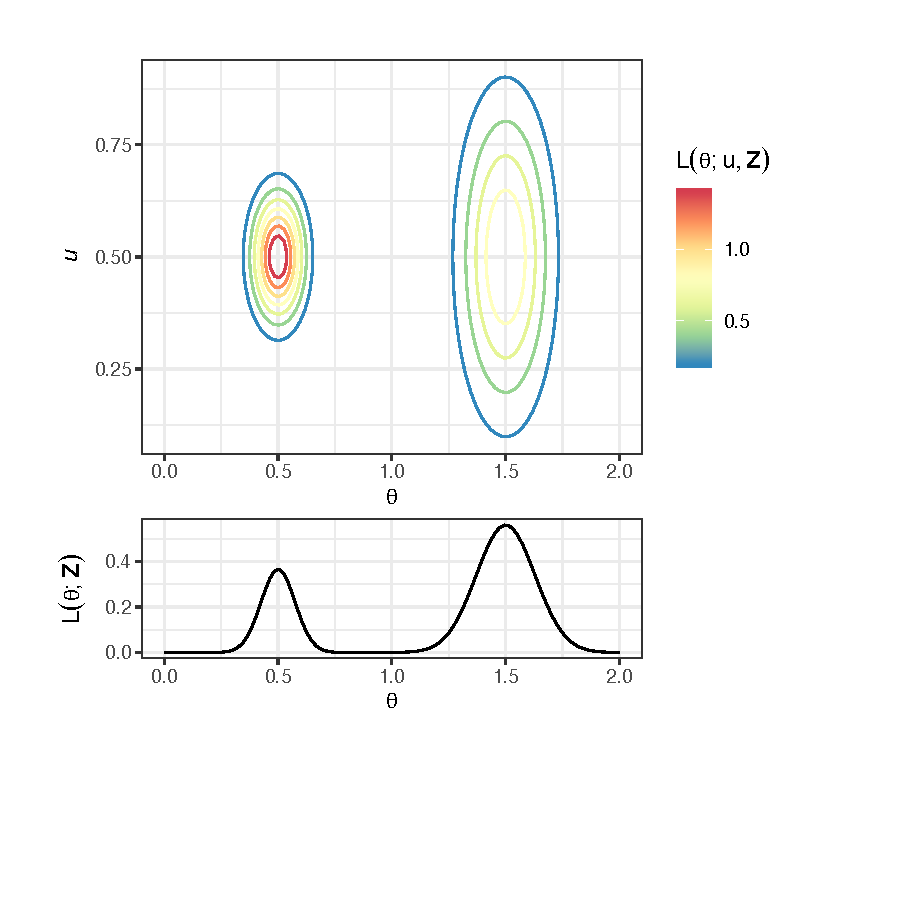
\includegraphics[width = 0.75\linewidth]{results/02-TwoProbMass.png}
%     \caption[Two regions of probability mass, demonstrating the different estimates of $\vec{\theta}$ which result from maximising the observed-data and joint log-likelihood function]{Two regions of probability mass. The first, centred around $\theta = 0.5$, has a larger density than the second when $u$ is not marginalised out. However, the second, centred at $\theta = 1.5$, contributes more to the observed-data likelihood $L(\theta; \vec{Z})$. Hence, an estimate of $\theta$ based on the observed-data likelihood would yield $\hat{\theta} = 1.5$ and not $\hat{\theta} = 0.5$.}
%   \label{fig:02-04:TwoProbMass}
% \end{figure}



% \begin{figure}[t!]
%     \centering
%     \begin{subfigure}[b]{\linewidth}
%         \centering
%         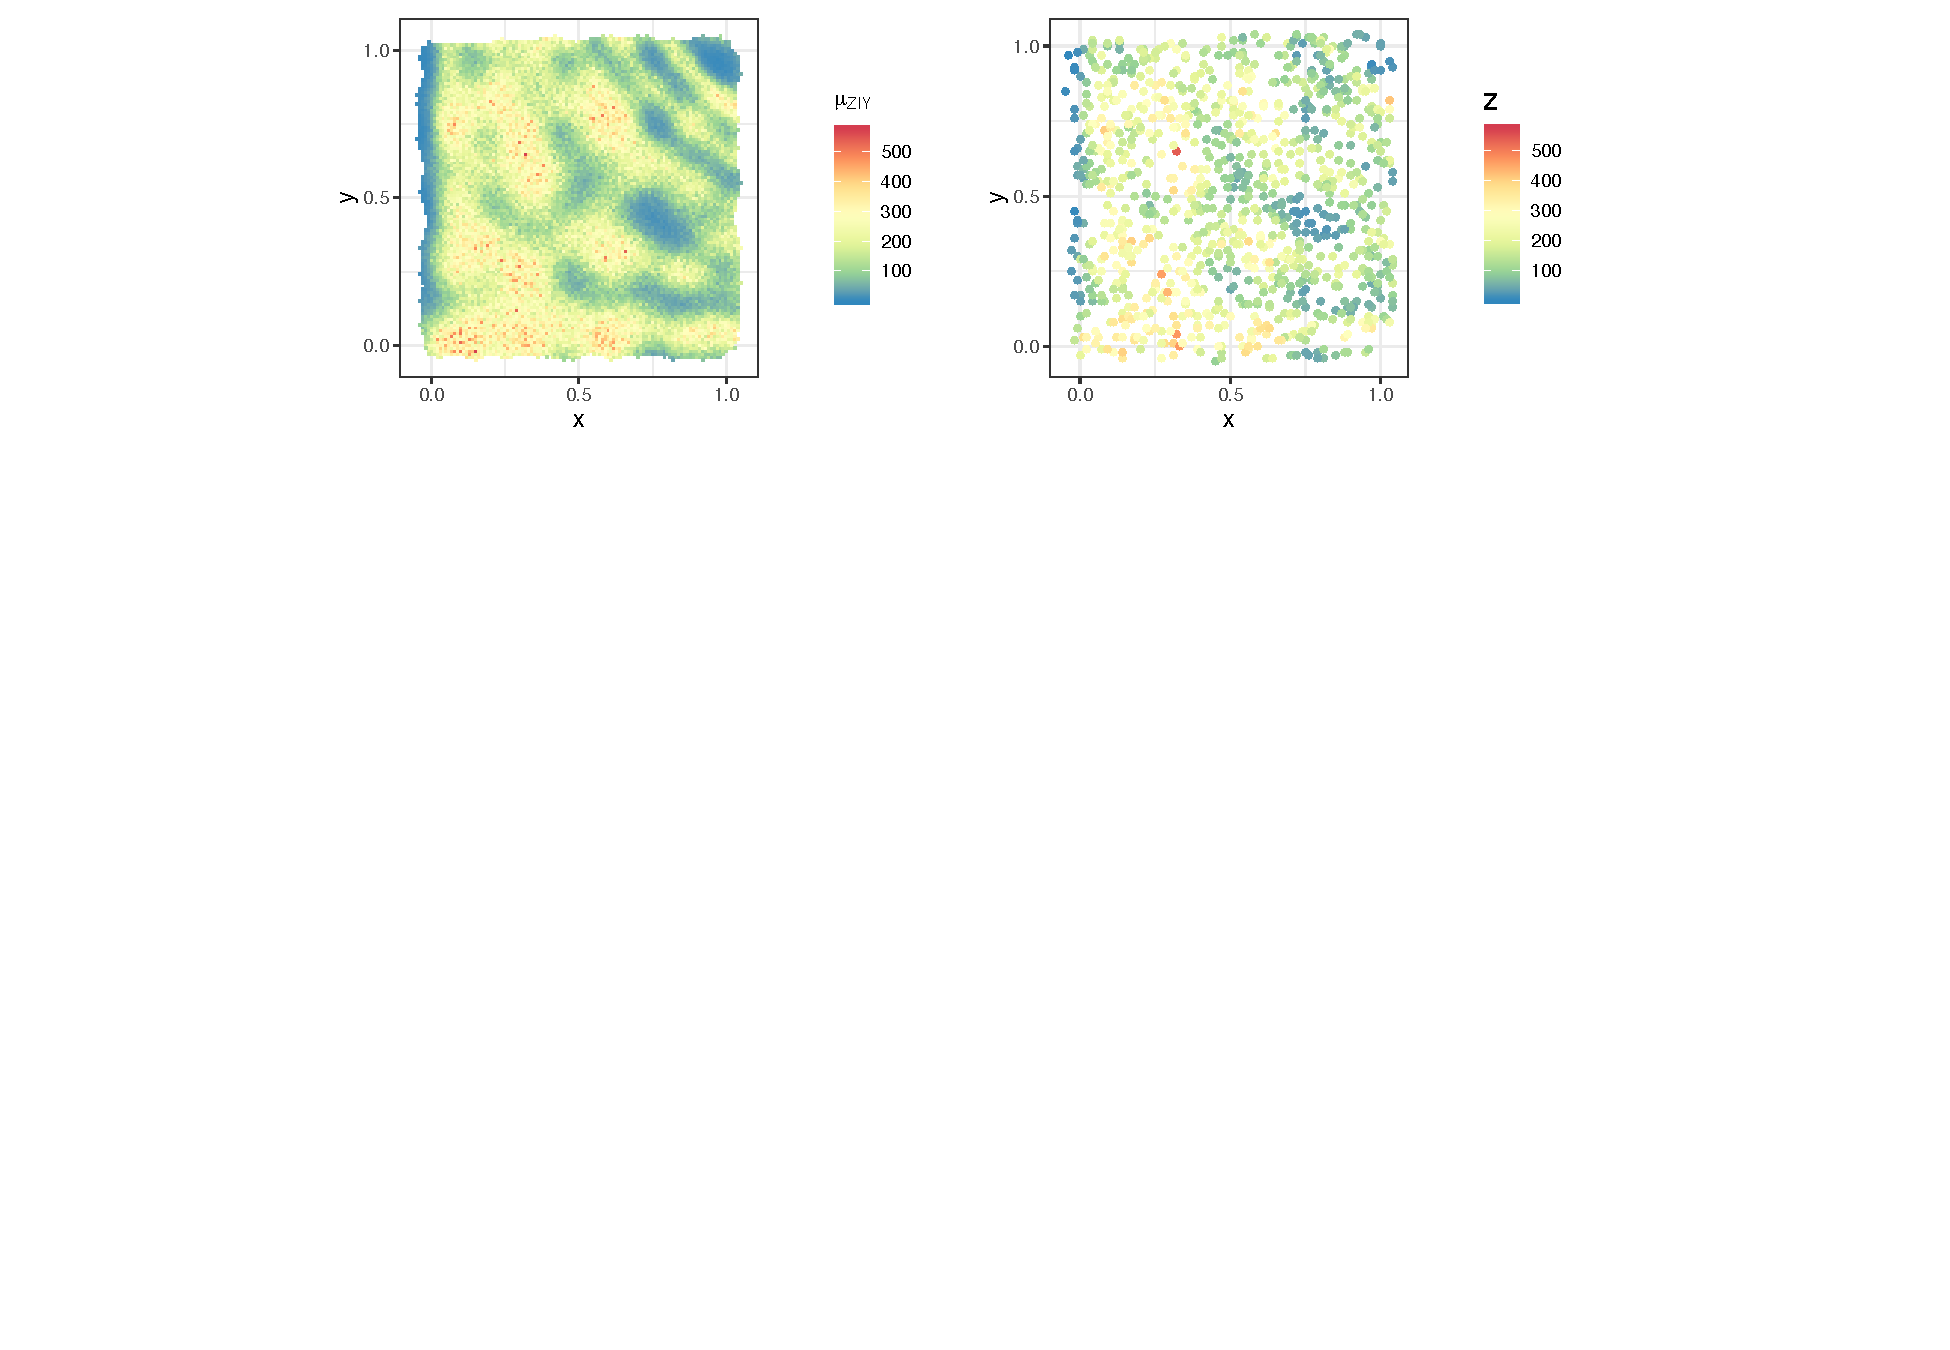
\includegraphics[width=\linewidth]{results/03-02-Poisson_plots2a.png}
%         \caption{(Left panel) True conditional mean of the data, $\mu(\cdot)$. (Right panel) Observed data.}\label{fig:03-02-PoissonResA}
%         \vspace{2\baselineskip}
%     \end{subfigure}
%     \begin{subfigure}[b]{\linewidth}
%         \centering
%         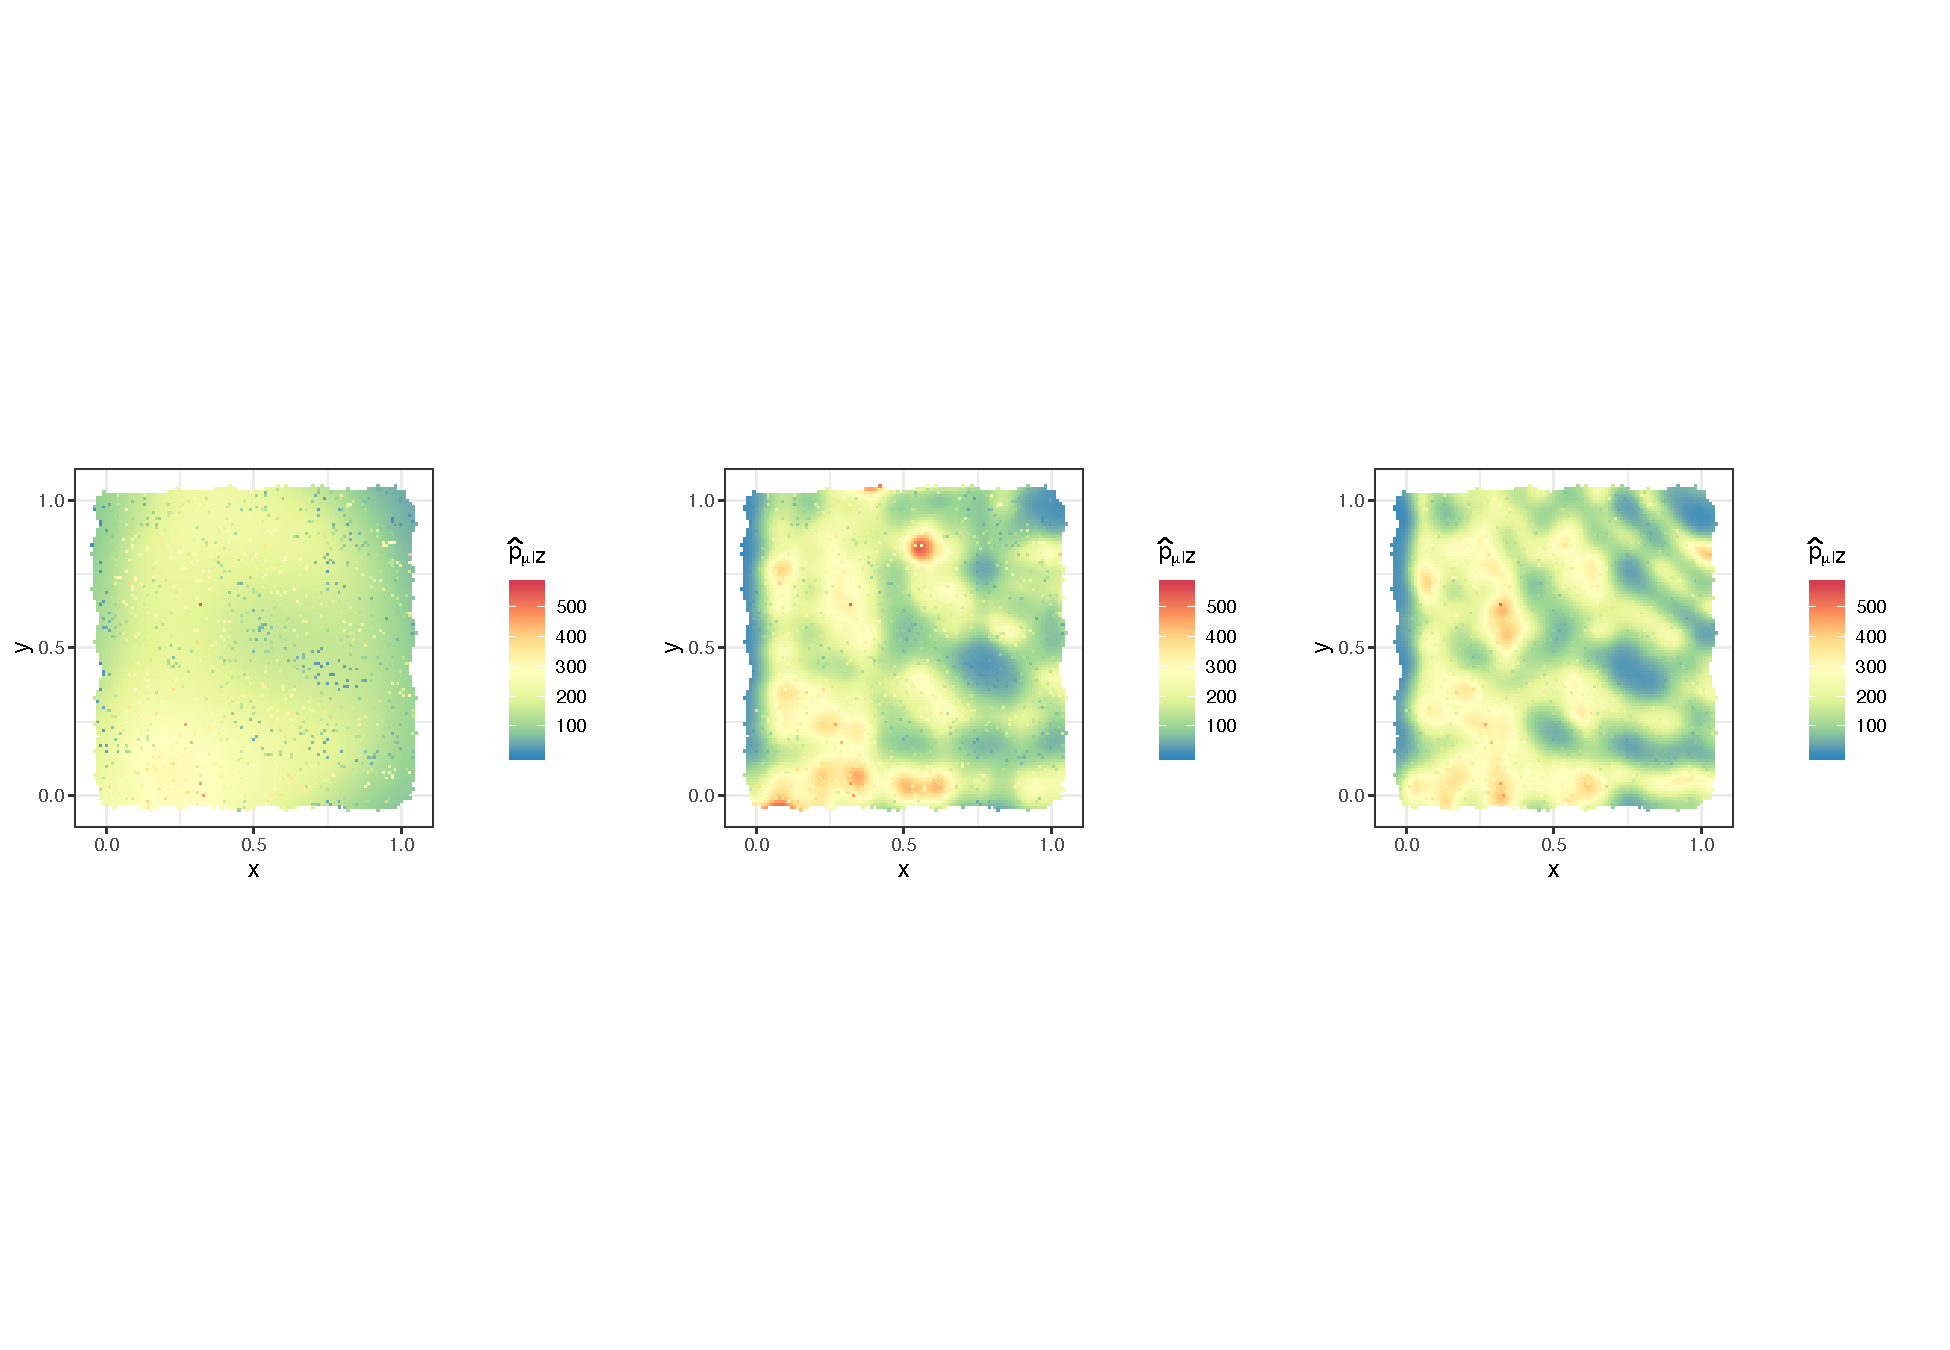
\includegraphics[width=\linewidth]{results/03-02-Poisson_plots2b.png}
%         \caption{Prediction maps using basis functions of one resolution (left panel), two resolutions (centre panel), and three resolutions (right panel).}\label{fig:03-02-PoissonResB}
%         \vspace{2\baselineskip}
%     \end{subfigure}
%         \begin{subfigure}[b]{\linewidth}
%         \centering
%         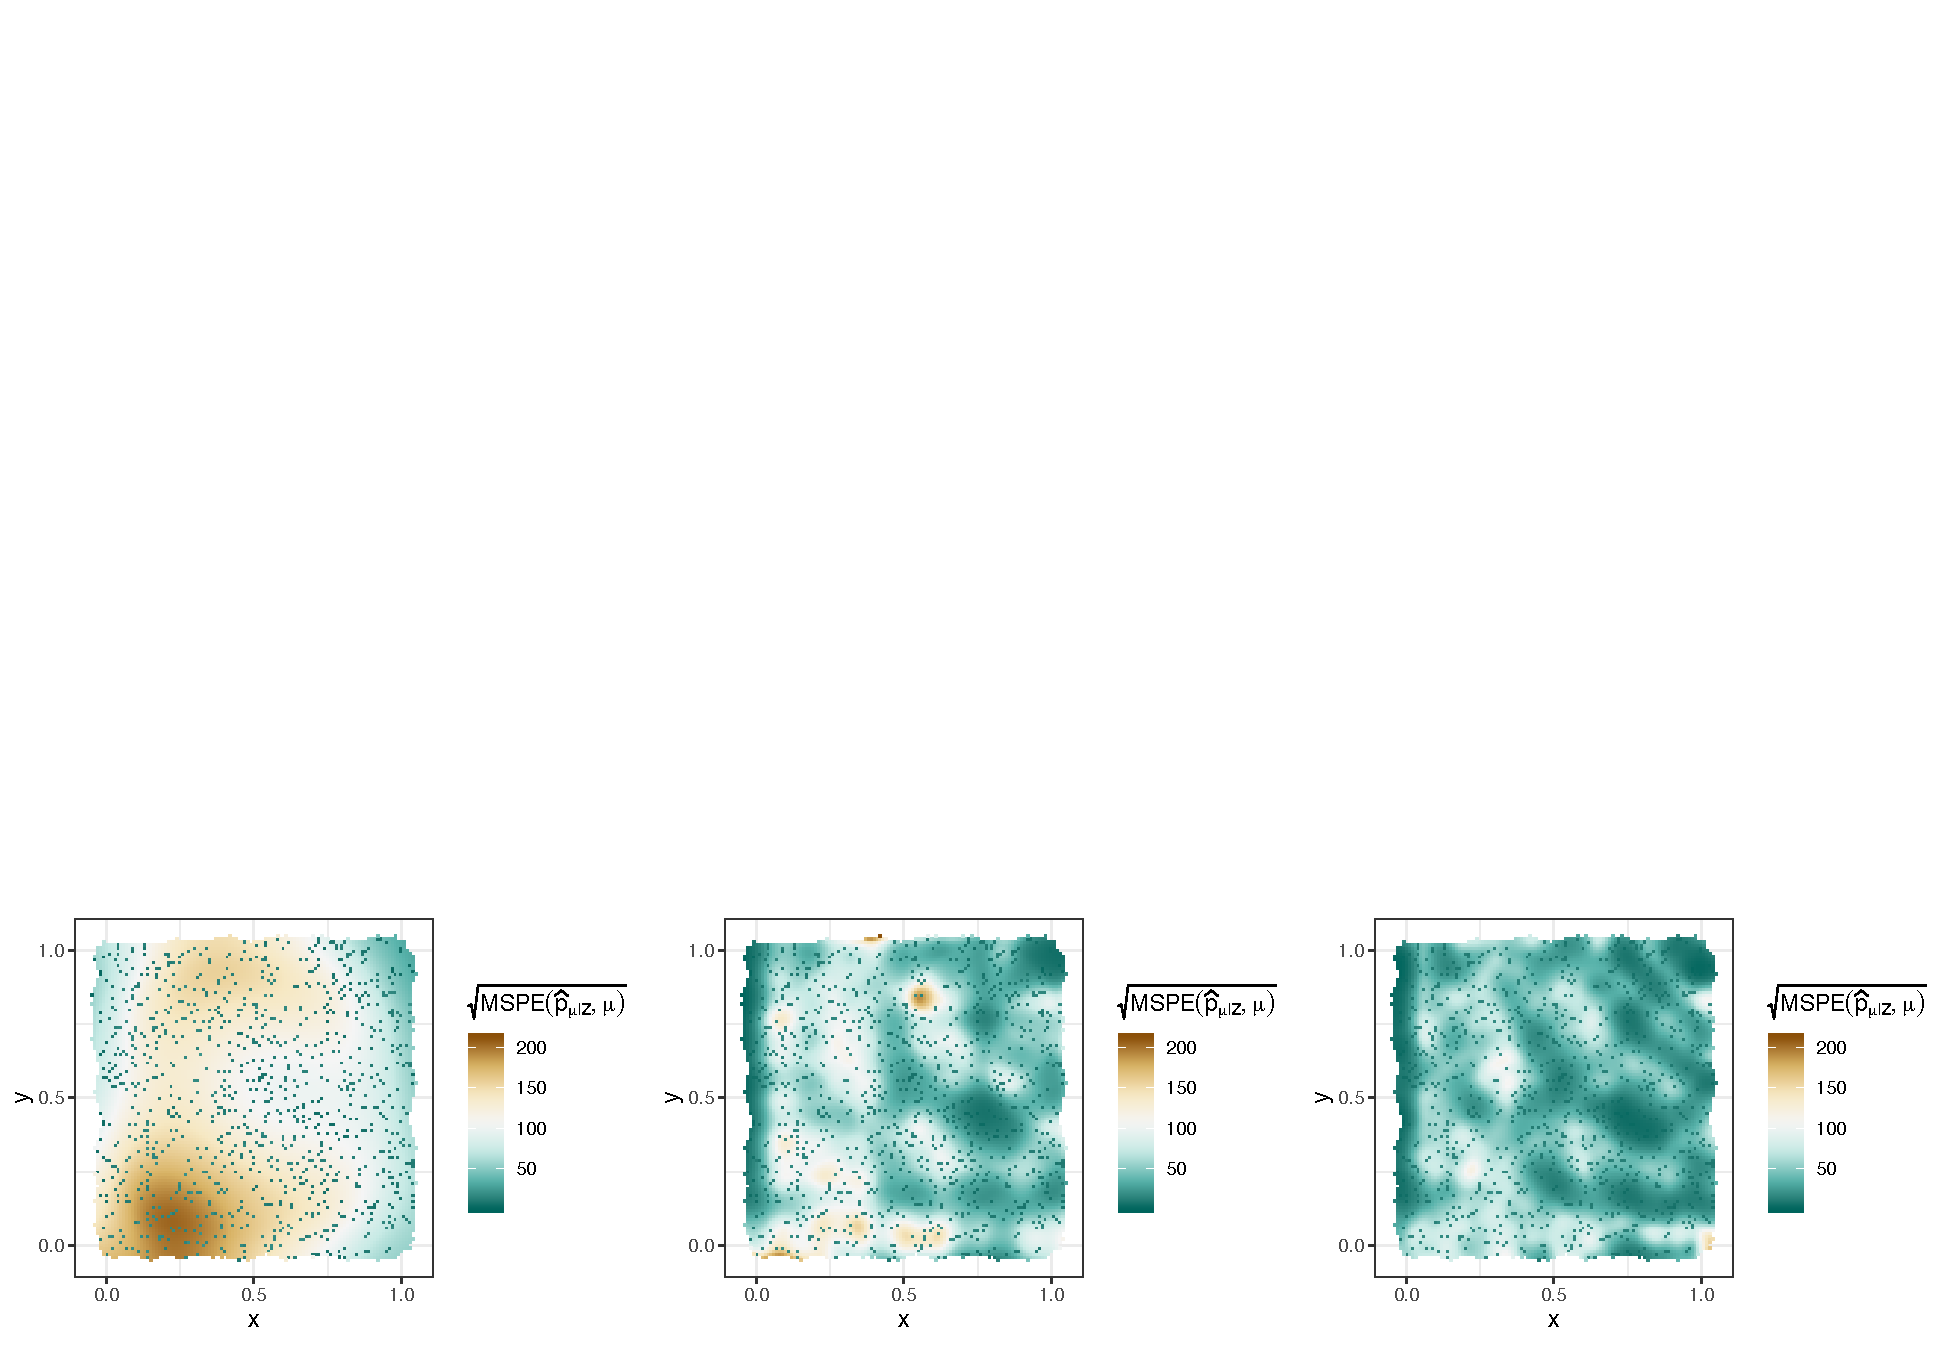
\includegraphics[width=\linewidth]{results/03-02-Poisson_plots2c.png}
%         \caption{Prediction uncertainty maps using basis functions of one resolution (left panel), two resolutions (centre panel), and three resolutions (right panel).}\label{fig:03-02-PoissonResC}
%         \vspace{2\baselineskip}
%     \end{subfigure}
%     \caption{Several panels summarising the analysis of a Poisson data set using one, two, and three resolutions of basis functions. Clearly, detail of our predictions increases with an increasing number of resolutions used; this is apparent by comparing the smooth, relatively uniform prediction and uncertainty maps created using one resolution, to the more intricate maps generated using three resolutions. The prediction uncertainty also decreases as we use more basis functions.}
%     \label{fig:03-02-PoissonRes}
% \end{figure}



%\begin{figure}[t!]
%    \centering
%    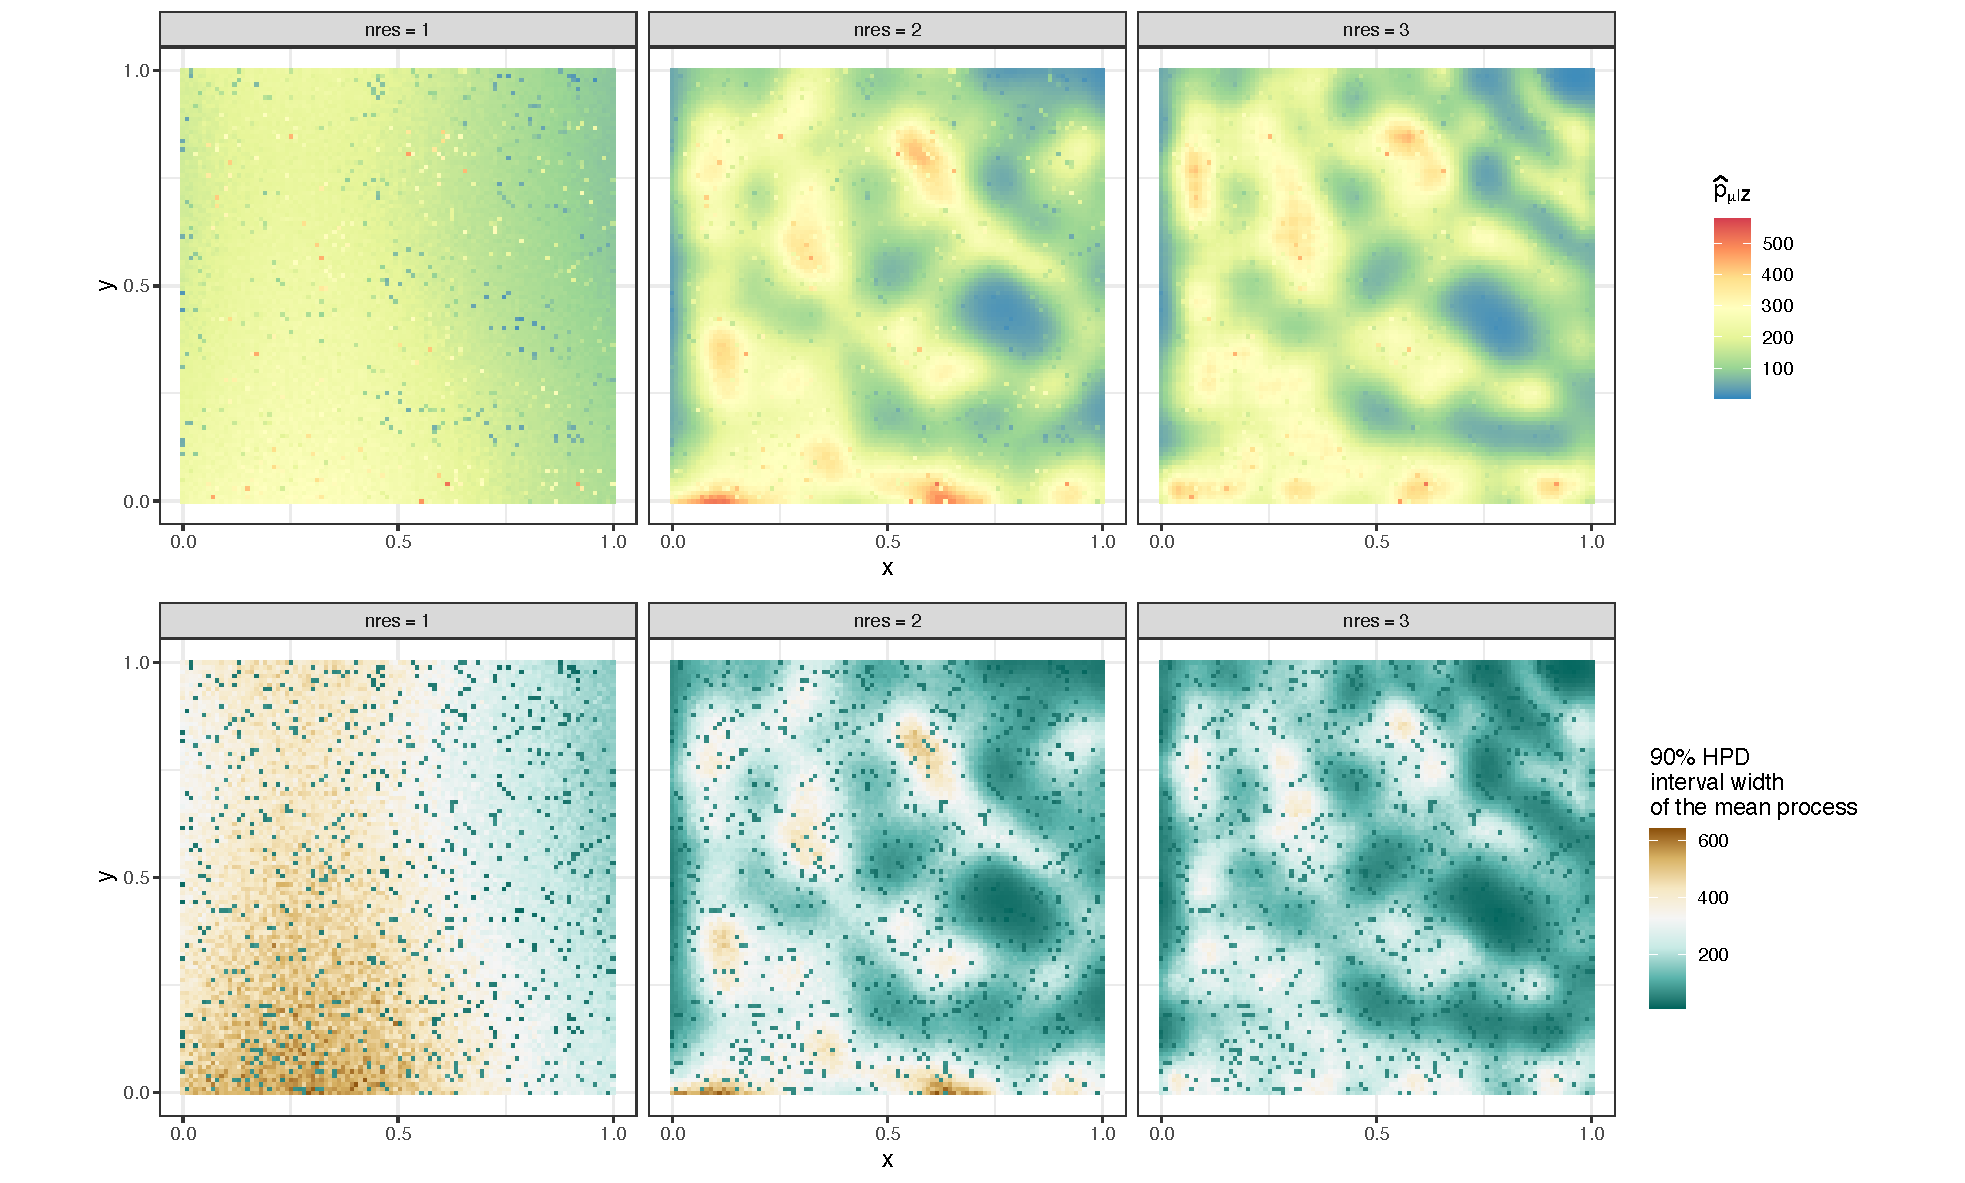
\includegraphics[width = \linewidth]{results/Poisson_multires.png}
%    \caption{Prediction and prediction uncertainty when analysing the Poisson data shown in Figure \ref{fig:Poisson_true_and_Z}. The first row corresponds to predictions of the mean process, $\mu(\cdot)$, while the second row corresponds to prediction uncertainty. The figure is divided into three columns, with the first, second, and third columns corresponding to predictions using one, two, and three resolutions of basis functions, respectively. 
%}   
%  \label{fig:Poisson_multires}
%\end{figure}


%\begin{figure}
%    \centering
%    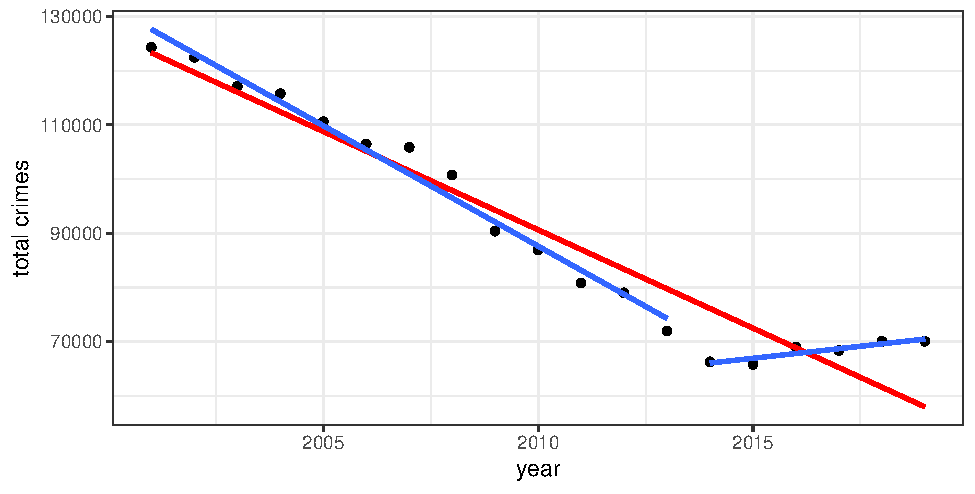
\includegraphics[width = 0.7\linewidth]{results/temporal_trend.png}
%    \caption{The total number of crimes committed across Chicago in each year, as well as two sets of fitted lines: the \red{red} line corresponds to a linear model that considers all data simultaneously, whilst the \textcolor{blue}{blue} line corresponds to a piece-wise linear model split by the year 2014. The improved fit using a piece-wise linear model suggests a piece-wise temporal trend is appropriate for the Chicago analysis presented in Section \ref{sec:ST_example}.}   
%  \label{fig:chicago_temporal_trend}
%\end{figure}



\newpage

\addtocontents{toc}{\protect\setcounter{tocdepth}{1}} % set only sections
\numberwithin{equation}{section}


\begin{appendix}

\section[Parameterisations of K and Q]{Parameterisations of $\vec{K}$ and $\vec{Q}$}\label{Appendix:CovarianceTapering}

Recall from Section \ref{subsection:04-01:ProcessLayer} that \pkg{FRK} v2 allows the covariance matrix of basis-function coefficients, $\vec{\eta}$, to be parameterised using either a covariance matrix, $\vec{K}$, or using a precision matrix, $\vec{Q}$.  
 In this appendix, we describe the parameterisation of these matrices.
 Both $\vec{K}$ and $\vec{Q}$ are block-diagonal matrices, wherein basis-function coefficients within a basis-function resolution are dependent, but independent between different resolutions. Hence, $\vec{K}$ and $\vec{Q}$ are fully defined via their intra-resolution dependencies. 
 
\subsection[Covariance matrix K]{Covariance matrix $\vec{K}$}\label{Appendix:CovarianceTapering:covariance_matrix_K}


 Let $K_k(\vec{s}, \vec{s}^*)$ denote the covariance function associated with the basis-function coefficients corresponding to the $k$th basis-function resolution. 
 In \pkg{FRK} v1/v2, we let $K_k(\vec{s}, \vec{s}^*)$ be the exponential covariance function, that is, 
\begin{equation}\label{eqn:02-01:K_covariance_function}
    K_k(\vec{s}, \vec{s}^*)  = \sigma^2_k \exp \left\{\frac{-d(\vec{s},\vec{s}^*)}{\tau_k}\right\}, 
\end{equation}
where $d(\vec{s},\vec{s}^*)$ is the distance between two basis-function centroids $\vec{s}, \vec{s}^* \in D$, $\sigma^2_k$ is a variance parameter, and $\tau_k$ is a length-scale parameter.  The $k$th sub-block of $\vec{K}$ is formed by evaluating \ref{eqn:02-01:K_covariance_function} for all pairs of basis-function centroids at the $k$th resolution.


Clearly (\ref{eqn:02-01:K_covariance_function}) is always non-zero for $\sigma^2_k > 0$, however 
 it is often reasonable to assume that coefficients associated with fine-resolution basis functions separated by medium-to-large distances are uncorrelated. 
To increase sparsity, \pkg{FRK} v2 now allows covariance tapering \citep{Furrer_2006_CovarianceTapering} of the intra-resolution covariance function. 
 Noting that (\ref{eqn:02-01:K_covariance_function}) is a special case of the Matérn covariance function with Matérn smoothness parameter $\nu = 0.5$, we follow the recommendation of \cite{Furrer_2006_CovarianceTapering} and use the spherical taper: 
\begin{equation}\label{eqn:02-01:taper_function}
%K_{\beta_k}(\vec{s}, \vec{s}^*) 
T_{\beta_k}(\vec{s}, \vec{s}^*) 
=
\left\{1-\frac{d(\vec{s},\vec{s}^*)}{\beta_k}\right\}^2_{+}   \left\{1+\frac{d(\vec{s},\vec{s}^*)}{2\beta_k}\right\},
\end{equation}
where $x_{+} \equiv \max(0, x)$, and $\beta_k$ is a resolution-dependent tapering parameter controlling the strength of the taper. 
 In \pkg{FRK} v2, we let $\beta_k$ be proportional to the minimum distance between basis-function centroids; specifically, we set $\beta_k = \texttt{taper} \times \text{mindist}(k)$, where $\text{mindist}(k)$ is the minimum distance between the centroids of basis functions at the $k$th resolution and \code{taper} is a user-specified argument.
The tapered covariance function is obtained by taking the product of the original covariance function (\ref{eqn:02-01:K_covariance_function}) and the taper function (\ref{eqn:02-01:taper_function}).
% Element wise product of the covaiance matrix and taper matrix


\subsection[Precision matrix Q]{Precision matrix $\vec{Q}$}

\pkg{FRK} v2 offers two types of sparse precision matrices: One is for regularly spaced basis functions, and the other is for irregularly spaced basis functions. 
 This choice is determined by the slot \code{regular} in the \class{Basis} object.

%When the basis functions are regularly spaced (\code{regular = TRUE}), \pkg{FRK} v2 uses a precision matrix that is related to that used in the \proglang{R} package \pkg{LatticeKrig} \citep{Nychka_2016_LatticeKrig}. 
% Let $\mathcal{N}_{i,k}$ denote the set of first-order horizontal and vertical neighbouring basis functions of the $i$th basis function of resolution $k$, 
%%The number of elements in $\mathcal{N}_{ik}$, $|\mathcal{N}_{i,k}|$, will be four for interior basis functions, three for basis functions on edges, and two for basis functions on corners when the basis functions are arranged on a regular grid in $\mathbb{R}^2$.
% and let $\vec{Q}_k$ denote the precision matrix of the basis-function coefficients at resolution $k$. 
 
 \looseness=-1
 When the basis functions are regularly spaced (\code{regular = TRUE}), \pkg{FRK} v2 uses a precision matrix based on the Leroux model \citep{Leroux_2000_two_parameter_autoregressive_model}. 
Let $\mathcal{N}_{i,k}$ denote 
 the set of  %%% PREVENT ORPHAN/WIDOW
 first-order horizontal and vertical neighbouring basis functions of the $i$th basis function of resolution $k$, 
%The number of elements in $\mathcal{N}_{ik}$, $|\mathcal{N}_{i,k}|$, will be four for interior basis functions, three for basis functions on edges, and two for basis functions on corners when the basis functions are arranged on a regular grid in $\mathbb{R}^2$.
 and let $\vec{Q}_k$ denote the precision matrix of the basis-function coefficients at resolution $k$.  

We model the elements of $\vec{Q}_k$ as
\begin{equation}\label{eqn:Q_k}
    \{\vec{Q}_{k}\}_{i, j}
=
\begin{cases}
\kappa_k + \rho_k |\mathcal{N}_{i,k}|   & i = j\\
-\rho_k & j \in \mathcal{N}_{i,k} \\
0 & \text{otherwise}
\end{cases},
\end{equation}
where $\kappa_k$ and $\rho_k$ are parameters that are estimated. 
%The full precision matrix $\vec{Q}$ is then $\text{bdiag}(\{\vec{Q}_k: k = 1,...,l\})$, where $l$ is the number of basis-function resolutions, and $\text{bdiag}(\cdot)$ returns a block-diagonal matrix from its arguments. 
We note that $\vec{Q}_k$ is diagonally dominant, and hence it is positive-definite. 
 This formulation implies that the coefficient of a given basis function is conditionally independent of all other basis-function coefficients given the coefficients of its first-order vertical and horizontal neighbours. 
% Note that \cite{Leroux_2000_two_parameter_autoregressive_model} used a model that is closely related to (\ref{eqn:Q_k}), and that \pkg{LatticeKrig} uses $\vec{Q}_k^\tp\vec{Q}_k$ as the precision matrix blocks, whereas \pkg{FRK} v2 uses $\vec{Q}_k$.  
Note that \pkg{LatticeKrig} uses $\vec{Q}_k^\tp\vec{Q}_k$ as the precision matrix blocks, whereas \pkg{FRK} v2 uses $\vec{Q}_k$.  





 To cater for irregularly-spaced basis functions, \pkg{FRK} v2 also offers a sparse precision matrix based on the distance between basis-function centroids:  
\begin{equation}\label{eqn:K_type_precision-block-exponential}
\{\vec{Q}_{k}\}_{i, j}
=
\begin{cases}
\kappa_k -\sum_{l \neq i}\{\vec{Q}_{k}\}_{i, l}  & i = j\\
-\rho_k \exp \left\{\frac{-d(\vec{s}_{i, k}, \vec{s}_{j, k})}{\tau_k}\right\}
    T_{\beta_k}(\vec{s}_{i, k}, \vec{s}_{j, k})  & i \neq j\\
\end{cases},
\end{equation}
where $\kappa_k$, $\rho_k$, and $\kappa_k$ are parameters that are estimated, and $T_{\beta_k}(\cdot, \cdot)$ is defined as in Appendix \ref{Appendix:CovarianceTapering:covariance_matrix_K}. 
 Again, this matrix is diagonally dominant and hence is positive-definite. 
 This formulation implies that the partial correlation between basis-function coefficients decays exponentially with distance until a point (controlled by the tapering parameter $\beta_k$) at which the basis-function coefficients are conditionally independent. 





%\section{Prediction}\label{app:prediction}
%
%\numberwithin{equation}{subsection}
%
%
%In this appendix, we provide details for how we predict the latent process $Y(\cdot)$, the mean process $\mu(\cdot)$, and the noisy data process. 
%%For simplicity, we provide details for the simple kriging case, whereby the fixed-effects $\vec{\alpha}$ are assumed to be known quantities, with the uncertainty of their estimation unaccounted for.
%%The universal kriging case, which, in this framework, involves treating $\vec{\alpha}$ as random quantities, is a straightforward extension. 
%For notational convenience, we treat the regression parameters, $\vec{\alpha}$, as known.
%
%
%\subsection{Prediction of the latent process}\label{sec:04-03-01:YProcessPrediction}
%
%
%The predictor of $Y_i$, the latent process $Y(\cdot)$ evaluated over the BAU $A_i$, is the expectation of $Y_i$ conditional on the data, parameters, and fixed effects;
%\begin{equation}\label{eqn:02-03:pYgivenZ}
%    \pYgivenZ{A_i}
%    \equiv
%    \ECurly{Y_i \mid \vec{Z}, \vec{\theta}}.
%\end{equation}
%Recall from Section 
%%\ref{sec:observed-data_likelihood} 
%\ref{subsection:02-03:Estimation} 
% that the posterior distribution of the random effects, $\vec{u} \equiv (\vec{\eta}^\tp, \vec{\xi}^\tp)^\tp$, is approximated to be Gaussian (as we use the Laplace approximation), and hence the posterior distribution of $Y_i$ is also approximated to be Gaussian.
%Therefore, another quantity of interest is the posterior variance;
%\begin{equation}\label{eqn:02-03:varYgivenZ}
%    \varCurly{Y_i \mid \vec{Z}, \vec{\theta}}.
%\end{equation}
%Given estimates of the posterior expectation and precision matrix of $\vec{u}$ using \pkg{TMB}, we can compute (\ref{eqn:02-03:pYgivenZ}) and (\ref{eqn:02-03:varYgivenZ}) in at least two ways. 
% The first is an analytic approach using basic expectation and variance properties, and the second is via Monte Carlo simulation.
%
%
%
%\subsubsection{Analytic approach}
%
%%Recall that for a location $\vec{s}\in D$, the process layer, irrespective of the assumed distribution of the data, is given by
%%\[
%%Y(\vec{s}) = \vec{t}(\vec{s})^\tp\vec{\alpha} + \phi(\vec{s})^\tp \vec{\eta} + \xi(\vec{s}); \quad \vec{s} \in D.
%%\]
%%Forms for the posterior expectation and variance can be derived straightforwardly. 
%% However, before doing so, we explore a fact that will simplify some terms considerably. 
%
%Recall that the process layer, irrespective of the assumed distribution of the data, is given by (\ref{eqn:04-01:Y(s)}). Defining $\vec{\xi}_O$ and $\vec{\xi}_U$ as the elements of $\vec{\xi}$ associated with observed and unobserved BAUs, respectively, it can be shown \citep[e.g.,][]{Sengupta_Cressie_2013_spatial_GLMM_FRK} that $\vec{\xi}_U$ are conditionally independent of all other random quantities in the model; that is, $[\vec{\xi}_U \mid \vec{Z}, \vec{\eta}, \vec{\xi}_O, \vec{\theta}] = [\vec{\xi}_U \mid \sigma^2_\xi]$. 
%%Define $\vec{\xi}_O$ and $\vec{\xi}_U$ as the elements of $\vec{\xi}$ associated with observed and unobserved BAUs, respectively.
%%\cite{Sengupta_Cressie_2013_spatial_GLMM_FRK} showed that, under the framework of a spatial GLMM with a spatial mixed effects model for the process layer, and assuming the fine-scale variation terms $\vec{\xi}$ are independent a priori, the unobserved fine-scale variation terms, $\vec{\xi}_U$, are conditionally independent of all other random quantities in the model; that is, that $[\vec{\xi}_U \mid \vec{Z}, \vec{\eta}, \vec{\xi}_O, \vec{\theta}] = [\vec{\xi}_U \mid \sigma^2_\xi]$.
%%This allows for considerable simplification of the posterior expectation and variance at unobserved locations. 
%%Specifically, (\ref{eqn:02-03:pYgivenZ}) becomes 
%Then, the posterior expectation (\ref{eqn:02-03:pYgivenZ}) is 
%\begin{align*}
%    \pYgivenZ{A_i}
%    &=
%    \ECurly{Y_i \mid \vec{Z}, \vec{\theta}}\\
%    &=
%    \vec{t}(A_i)^\tp\vec{\alpha} + \vec{\phi}(A_i)^\tp \E{\vec{\eta} \mid \vec{Z}, \vec{\theta}} + \ECurly{\xi_i \mid \vec{Z}, \sigma^2_\xi}\\
%    &=
%    \begin{cases} 
%      \vec{t}(A_i)^\tp\vec{\alpha} + \vec{\phi}(A_i)^\tp \E{\vec{\eta} \mid \vec{Z}, \vec{\theta}} + \ECurly{\xi_i \mid \vec{Z}, \sigma^2_\xi} & A_i\in D^O \\
%      \vec{t}(A_i)^\tp\vec{\alpha} + \vec{\phi}(A_i)^\tp \E{\vec{\eta} \mid \vec{Z}, \vec{\theta}} & A_i\notin D^O
%   \end{cases},
%\end{align*}
%where recall that $D^O$ denotes the set of observations supports. 
% The posterior variance (\ref{eqn:02-03:varYgivenZ}) is 
%\begin{align*}
%    &\varCurly{Y_i \mid \vec{Z}, \vec{\theta}} \nonumber \\
%    &=
%    \varCurly{\vec{\phi}(A_i)^\tp \vec{\eta} \mid \vec{Z}, \vec{\theta}}
%    +
%    \varCurly{\xi_i \mid \vec{Z}, \sigma^2_\xi}
%    +
%    2 \covCurlyConditional{ \vec{\phi}(A_i)^\tp\vec{\eta}}{\xi_i }{ \vec{Z}, \vec{\theta} } \nonumber \\
%    &=
%    \vec{\phi}(A_i)^\tp\vec{\Sigma}_{\vec{\eta} \mid \vec{Z}}\vec{\phi}(A_i)
%    +
%    \varCurly{\xi_i \mid \vec{Z}, \sigma^2_\xi}
%    +
%    2\vec{\phi}(A_i)^\tp
%     \covCurlyConditional{ \vec{\eta} }{\xi_i }{\vec{Z}, \vec{\theta}} \nonumber \\
%    &=
%    \begin{cases}
%    \vec{\phi}(A_i)^\tp\vec{\Sigma}_{\vec{\eta} \mid \vec{Z}}\vec{\phi}(A_i)
%    +
%    \varCurly{\xi_i \mid \vec{Z}, \sigma^2_\xi}
%    +
%    2\vec{\phi}(A_i)^\tp
%    \covCurlyConditional{ \vec{\eta} }{ \xi_i }{ \vec{Z}, \vec{\theta} } & A_i\in D^O\\
%    \vec{\phi}(A_i)^\tp\vec{\Sigma}_{\vec{\eta} \mid \vec{Z}}\vec{\phi}(A_i)
%    +
%    \sigma^2_\xi & A_i\notin D^O
%    \end{cases},
%\end{align*}
%where $\vec{\Sigma}_{\vec{\eta} \mid \vec{Z}}$ is the posterior covariance matrix of the basis-function random coefficients.  
%%Hence, for prediction and prediction uncertainty quantification of $Y_i$, we require the posterior expectation and variances of $\vec{\eta}$ and $\vec{\xi}_O$, as well as their posterior covariances. 
%%Approximations of these values can be obtained using \pkg{TMB}. 
%The posterior expectation of $\vec{u}$ is immediately available upon conclusion of model fitting.  
% However, \pkg{TMB} provides the posterior \textit{precision} matrix of $\vec{u}$, which must be inverted to obtain variances and covariances. 
%The random effect block has dimension equal to the number of basis functions, $r$, plus the number of observed BAUs, $|D^O|$. 
%Since $r + |D^O|$ is usually large, obtaining the covariance matrix of the random effects directly can be computationally prohibitive. 
%We thus make use of the \textit{sparse-inverse-subset algorithm} (see \cite{Takahashi(1973)SparseInverseSubsetAlgorithm}; \cite{Rue_Martino_2007_Bayesian_inference_for_GMRF}; \cite{Zammit-Mangion_Rougier_2018_sparse_inverse_subset}) to obtain only the necessary elements of the covariance matrix; the sparse-inverse-subset algorithm is implemented with the \proglang{R} package \pkg{sparseinv} \citep{sparseinv_Package}. 
%%This dramatically reduces the computational time to obtain the required posterior variances and covariances.
%
%
%In practice, we do not perform a single calculation at a time; we use a matrix-vector form. In particular, the term $\vec{\phi}(A_i)^\tp   \vec{\Sigma}_{\vec{\eta} \mid \vec{Z}}   \vec{\phi}(A_i)$ can be computed for all locations via 
%$$\diag{\vec{S} \vec{\Sigma}_{\vec{\eta} \mid \vec{Z}} \vec{S}^\tp} = \left(\vec{S} \vec{\Sigma}_{\vec{\eta}|\vec{Z}}\odot \vec{S}\right)\vec{1},$$
%where $\odot$ denotes element-wise multiplication.
%
%
%\subsubsection{Monte Carlo approach}
%
%Rather than computing the expectation and variance of $Y_i$ analytically, we may instead generate Monte Carlo samples of $Y_i$, and then approximate the expectation and variance by the sample mean and sample variance, respectively. 
%%Monte Carlo simulation is required when inference is desired on the mean process or the noisy data (with some exceptions outlined in Section \ref{sec:prediction_mean_process}). 
%%; namely, when the link function is the identity or log function, and when the data are Gaussian). %, and it may be useful if employing the sparse-inverse-subset algorithm is deemed to have a non-negligible effect on inference. 
%Denote the posterior mode and precision matrix of the random effects by $\hat{\vec{u}}$ and $\vec{Q}_{u}$, respectively. 
%Our approach involves simulating from the $\Gau(\hat{\vec{u}}, \vec{Q}_{u})$ distribution in order to generate Monte Carlo samples of $\vec{Y}$.
%%
%%Define a permuted version of the precision matrix as $\vec{A} \equiv \vec{P}^\tp \vec{Q}_{u} \vec{P}$, where $\vec{P}$ is a permutation matrix. Define the upper Cholesky factor of $\vec{A}$ as $\vec{U}_P$, which is the upper triangular matrix satisfying $\vec{A} = \vec{U}_P^\tp \vec{U}_P$. Then, we have that $\vec{Q}_{u} = \vec{M}^\tp \vec{M}$, where $\vec{M} = \vec{U}_P \vec{P}^\tp$ is \textit{not} triangular.
%%Now consider the usual method of transforming a standard Gaussian vector to a Gaussian vector with precision matrix $\vec{Q}_{u}$. 
%%First, let $\vec{z} \sim \Gau(\vec{0}, \vec{I})$ denote a standard Gaussian random vector. Then, we have that the variance of the transformed vector $\tilde{\vec{u}} \equiv \vec{M}^{-1}\vec{z} $ is
%%\begin{align*}
%%    \var{\tilde{\vec{u}}}
%%    = \var{\vec{M}^{-1}\vec{z}}
%%    = \vec{M}^{-1}\vec{M}^{-\tp}
%%    = (\vec{M}^{\tp}\vec{M})^{-1}
%%    = \vec{Q}_{u}^{-1},
%%\end{align*}
%%as required. Note, however, that although $\vec{M}$ is sparse, it is not triangular.
%%However, we have that $\vec{M}^{-1} = \vec{P} \vec{U}_P^{-1}$,
%%and so $\tilde{\vec{u}}$ may equivalently be written as
%%$\tilde{\vec{u}} = \vec{P} \vec{U}_P^{-1}\vec{z}$.
%%Therefore, we can first solve the upper triangular system $\vec{U}_P \vec{x} = \vec{z}$, and then left-multiply $\vec{x}$ by the permutation matrix $\vec{P}$ to obtain $\tilde{\vec{u}} = \vec{P} \vec{x} = \vec{P} \vec{U}_P^{-1}\vec{z} = \vec{M}^{-1}\vec{z}$, as required. 
%%This approach to generating samples fully exploits both the reduction of fill-in from matrix reordering, as well as a computationally efficient backward-solve.
%%
%Once we have generated $n_{\text{MC}}$ samples of $\vec{u}$, we construct $\vec{Y}_{\!\text{MC}}$, an $N \times n_{\text{MC}}$ matrix whose $i$th row contains $n_{\text{MC}}$ Monte Carlo samples of $Y_i$, via 
%\[
%\vec{Y} 
%= \vec{T}\vec{\alpha} + \vec{S}\vec{\eta} + \vec{\xi}
%= \vec{T}\vec{\alpha} + 
%%\begin{bmatrix}\vec{S} & \vec{I}\end{bmatrix} 
%[\vec{S} \; \vec{I}]
%\vec{u}
%.
%\]
%Then, we may estimate (\ref{eqn:02-03:pYgivenZ}) and (\ref{eqn:02-03:varYgivenZ}) by taking row-wise means and variances of $\vec{Y}_{\!\text{MC}}$. 
%%Further, samples from the mean process may be generated by passing the samples contained in $\vec{Y}^{MC}$ through the inverse-link function. 
%
%
%
%
%
%
%\subsection{Prediction of the mean process}\label{sec:prediction_mean_process}
%
%
%%Recall that the mean process, $\mu(\cdot)$, is modelled as a transformation of the latent process $Y(\cdot)$ via a link function $g(\cdot)$, so that $g\!\left(\mu(\cdot)\right) = Y(\cdot)$, or, equivalently,
%%\begin{equation}\label{eqn:04-03:mu=psi(Y)}
%%    \mu(\vec{s}) = g^{-1}\!\left(Y(\vec{s})\right), \quad \vec{s} \in D.
%%\end{equation}
%%Again, we use the posterior expectation as our predictor of (\ref{eqn:04-03:mu=psi(Y)}) at $A_i$;
%Again, as predictor of $\mu_i$, the mean process $\mu(\cdot)$ evaluated the BAU $A_i$, we use the posterior expectation;
%\begin{equation}\label{eqn:04-03:muOptimalPredictor}
%    \pmugivenZ{A_i} 
%    \equiv 
%    \ECurly{\mu_i \mid \vec{Z}, \vec{\theta}}.
%\end{equation}
%% Again using the general result (\ref{eqn:04-03:GeneralMSPE}), the MSPE of (\ref{eqn:04-03:muOptimalPredictor}) when predicting the conditional mean $\mu(\cdot)$ at $A_i$ is 
%% \begin{equation}\label{eqn:04-03:MSPEmuGivenZ_1}
%%     \MSPEtwoarg{\pmugivenZ{A_i}}{\mu(A_i)}
%%     =
%%     \ECurly{\var{\mu(A_i) \mid \vec{Z}}},
%% \end{equation}
%% which we again estimate by
%% \begin{equation}\label{eqn:04-03:MSPEmuGivenZ2}
%%     \MSPEtwoarg{\pmugivenZ{A_i}}{\mu(A_i)}
%%     \approx
%%     \varCurly{\mu(A_i) \mid \vec{Z}}
%% \end{equation} 
%% in the non-Gaussian case.
%%Note that the assumptions made on the latent process $Y(\cdot)$ do not change, irrespective of the assumed response distribution and link function combination. 
%%Hence, (\ref{eqn:02-03:pYgivenZ}) and (\ref{eqn:02-03:varYgivenZ}) remain as given in Section \ref{sec:04-03-01:YProcessPrediction} for all distributions and link functions supported by \pkg{FRK} v2. 
%Under certain link functions, (\ref{eqn:04-03:muOptimalPredictor}) may be evaluated analytically using (\ref{eqn:02-03:pYgivenZ}) and (\ref{eqn:02-03:varYgivenZ}). 
% This is trivially true for the identity link function.
%Under the log-link function, as we approximate $Y_i \mid \vec{Z}, \vec{\theta}$ to be Gaussian, $g^{-1}\!\left(Y_i\right) \mid \vec{Z}, \vec{\theta}$ approximately follows a \textit{log-normal} distribution.
%The expectation, variance, and quantile function (useful for uncertainty quantification) of a log-normal distribution are available in closed form. 
%Specifically, under the log-link, the predictor (\ref{eqn:04-03:muOptimalPredictor}) is
%\[
%    \pmugivenZ{A_i}
%    =
%    \exp\left(\ECurly{Y_i \mid \vec{Z}, \vec{\theta}} + \frac{\varCurly{Y_i \mid \vec{Z}, \vec{\theta}}}{2}\right),
%\]
%the posterior variance is
%\[
%    \varCurly{\mu(A_i) \mid \vec{Z}, \vec{\theta}}
%    =
%    \left(e^{\varCurly{Y_i \mid \vec{Z}, \vec{\theta}}}-1\right)
%    e^{2\ECurly{Y_i \mid \vec{Z}, \vec{\theta}}+\varCurly{Y_i \mid \vec{Z}, \vec{\theta}}},
%\]
%and the quantile function is
%\[
%Q(q)
%=
%\explr{
%\ECurly{Y_i \mid \vec{Z}, \vec{\theta}} + \sqrt{2 \varCurly{Y_i \mid \vec{Z}, \vec{\theta}}}
%\text{erf}^{-1}\!(2q - 1)
%},
%\]
%where $\text{erf}^{-1}\!(\cdot)$ denotes the inverse error function.
%
%
%When analytic solutions are not available, \pkg{FRK} v2 employs Monte Carlo simulation. 
%This is done by simulating samples of $Y_i$, and then transforming the samples via the mean function, $g^{-1}(\cdot)$. 
% In particular, we obtain Monte Carlo samples of $\vec{\mu}$, the mean process evaluated over the BAUs, via $\vec{M} \equiv g^{-1}(\vec{Y}_{\!\text{MC}})$, where $g^{-1}(\cdot)$ is applied element-wise.
% Posterior expectations, variances, and quantiles may then be computed straightforwardly. 
% 
%
%
%\subsection{Prediction of the noisy data process}
%
%We now turn our attention to prediction and prediction uncertainty of the noisy data process. 
%Again, we use the posterior expectation as our predictor; 
%\begin{equation}\label{eqn:04-03:ZOptimalPredictor}
%    \hat{p}_{Z_i|\vec{Z}}
%    \equiv 
%    \ECurly{Z_i \mid \vec{Z}, \vec{\theta}}.
%\end{equation}
%Using the law of total expectation, 
%% namely
%% \[
%% \E{A \mid B} = \ECurly{\E{A \mid B, C} \mid B}, 
%% \]
%we have that the predictor of $Z_i$ is
%\begin{align*}
%    \hat{p}_{Z_i|\vec{Z}}
%    &=
%    \ECurly{Z_i \mid \vec{Z}, \vec{\theta}}\\
%    &=
%    \ESquare{  \ECurly{Z_i \mid \vec{Z}, \vec{\theta}, \mu(A_i) }  \mid  \vec{Z}, \vec{\theta} }\\ 
%    &=
%    \ESquare{  \ECurly{Z_i \mid \mu(A_i)}  \mid  \vec{Z}, \vec{\theta} }\\
%    &=
%    \ESquare{  \mu(A_i)  \mid  \vec{Z}, \vec{\theta} }\\
%    &=
%    \pmugivenZ{A_i},
%\end{align*}
%and hence the predictor of $Z_i$ is equivalent to the predictor of the mean $\mu(A_i)$. 
%The posterior variance $\varCurly{Z_i \mid \vec{Z}, \vec{\theta}}$ can be derived using the law of total conditional variance \citep[e.g.,][]{Bowsher_Swain_2012_total_conditional_variance}, 
%% namely,
%% \begin{equation}\label{eqn:04-03:LawOfTotalConditionalVariance} 
%% \var{A \mid B} = \ECurly{\left.\var{A \mid B,C}\right|B} + \varCurly{\left.\E{A \mid B,C}\right|B},
%% \end{equation}
%so that
%\begin{align}\label{eqn:var(Z|Z)}
%    \varCurly{Z_i \mid \vec{Z}, \vec{\theta}}
%    &=
%    \ESquare{  \varCurly{  Z_i \mid \vec{Z}, \vec{\theta}, \mu_i    } \mid \vec{Z}, \vec{\theta}   } 
%    + 
%    \varSquare{  \ECurly{   Z_i \mid \vec{Z}, \vec{\theta}, \mu_i} \mid \vec{Z}, \vec{\theta}    }\nonumber\\
%    &=
%    \ESquare{   \varCurly{   Z_i \mid \mu_i   } \mid \vec{Z}, \vec{\theta}  } 
%    + 
%    \varSquare{ \ECurly{   Z_i \mid  \mu_i   } \mid \vec{Z}, \vec{\theta}}\nonumber\\
%    &=
%    \ESquare{   \varCurly{   Z_i \mid \mu_i   } \mid \vec{Z}, \vec{\theta}  } 
%    + 
%    \varCurly{ \mu(A_i) \mid \vec{Z}, \vec{\theta}}.
%\end{align}
%% This result makes intuitive sense. We have already shown that the predictors (\ref{eqn:04-03:muOptimalPredictor}) and (\ref{eqn:04-03:ZOptimalPredictor}) are equivalent, and so the difference in variance arises entirely from the differing variability of the predictands; a fact reflected by the term $\ESquare{   \varCurly{   Z_i \mid Y(A_i)   } \mid \vec{Z}  } $. Furthermore, it is well known that the uncertainty of an expectation is always lower than that of the corresponding data. 
%Under certain distributions, this expression simplifies further. For instance, when the data are assumed to follow a Poisson distribution, (\ref{eqn:var(Z|Z)}) simplifies to 
%\begin{align*}
% \varCurly{Z_i \mid \vec{Z}, \vec{\theta}}
%&=
%    \ECurly{\mu(A_i) \mid \vec{Z}, \vec{\theta}} 
%    + 
%    \varCurly{ \mu(A_i) \mid \vec{Z}, \vec{\theta}}\\
%&=
%\pmugivenZ{A_i}
%    + 
%    \varCurly{ \mu(A_i) \mid \vec{Z}, \vec{\theta}}.
%\end{align*}
% When analytic solutions are not available, \pkg{FRK} v2 again employs Monte Carlo simulation. 


%%%%%% C_ZC_pAppendix
\section[Incidence matrices: CZ and CP]{Incidence matrices: $\vec{C}_Z$ and $\vec{C}_P$}\label{Appendix:Incidence matrices: Cz and Cp}



Recall from Section \ref{subsection:DataLayer} that $\vec{C}_Z$ aggregates the BAU-level mean process, $\vec{\mu}$, over the observation supports and, depending on the weights in (\ref{eqn:C_Z}), it can correspond to a weighted average or a weighted sum over the BAUs. 
 In \pkg{FRK} v2, the weights $w_{ij}$ may be controlled through the argument \mbox{\code{normalise\_wts}} and the \code{wts} field of the \class{SpatialPixelsDataFrame}/\class{SpatialPolygonsDataFrame} object \citep{Pebesma_2005_sp_package} used to store the BAUs.  
 Specifically, the \code{wts} field allows one to attribute each BAU to a \textit{relative} weight $v_i$, $i = 1, \dots, N$, such that $w_{ij} \propto v_i$, where the constant of proportionality can vary with $j$.   
 For example, if the BAUs are of unequal area, then one may wish to set $v_i = |A_i|$. 
 By default (and implicit in \pkg{FRK} v1), each $v_i$ is set to 1. 
  The argument \mbox{\code{normalise\_wts}} controls whether $\vec{C}_Z$ corresponds to a weighted sum or a weighted average. If set to \code{FALSE}, then $w_{ij} = v_i$ for all $j$ (weighted sum); if set to \mbox{\code{TRUE}} (default and implicit in \pkg{FRK} v1), then the $\{w_{ij}\}$ are normalised so that each row of $\vec{C}_Z$ sums to 1 (weighted average) and $w_{ij} = v_i / \sum_{l \in c_j} v_l$.   
%  Note that if $v_i = |A_i|$ and \mbox{\code{normalise\_wts = TRUE}}, the $j$th row sum of $\vec{C}_Z$ is $\sum_{i \in c_j} |A_i| = |B_j|$, so that the normalised weights are $w_{ij} = |A_i|/|B_j|$.  
  Note that if $v_i = |A_i|$ and \mbox{\code{normalise\_wts = TRUE}}, the normalised weights are $w_{ij} = |A_i|/|B_j|$, since the BAUs are disjoint and $\sum_{i \in c_j} |A_i| = |B_j|$. 


Recall from Section \ref{subsection:Prediction} that $\vec{C}_Z$ aggregates the BAU-level mean process, $\vec{\mu}$, over the observation supports and, depending on the weights in (\ref{eqn:C_P}), it can correspond to a weighted average or a weighted sum over the BAUs. 
 Like $\vec{C}_Z$, the relative weights, $\{\tilde{v}_i: i = 1, \dots, N\}$, such that $\tilde{w}_{ik} \propto \tilde{v}_i$, are controlled by the \code{wts} field of the BAU object, and the argument \mbox{\code{normalise\_wts}} is used to control whether $\vec{C}_P$ represents a weighted sum or a weighted average. 
 For consistency between the model fitting and prediction stages, 
 \pkg{FRK} v2 enforces the use of the same relative weights, $\tilde{v}_i = v_i$ for $i = 1, \dots, N$, and the same setting of \code{normalise\_wts}, in construction of both $\vec{C}_Z$ and $\vec{C}_P$. 


 Recall from Section \ref{sec:Distributions with size parameters} that in most applications that consider binomial or negative-binomial data models, 
 the conditional mean of an observation is treated as a simple aggregate of the underlying mean process. 
 Therefore, with these distributions, \pkg{FRK} v2 enforces the matrix $\vec{C}_Z$ in (\ref{eqn:C_Z}) to be constructed with the relative weights \mbox{$\{v_i = 1$ : $i = 1, \dots, N\}$} and with \mbox{\code{normalise\_wts = FALSE}}, and hence $w_{ij} = 1$ in (\ref{eqn:C_Z}). 
 Then, the mapping from the BAU-level mean, $\vec{\mu}$, to the data-level mean, $\vec{\mu}_Z$, in (\ref{eqn:mu_Z}) is a simple, unweighted summation over the BAUs.  
 Since \pkg{FRK} v2 enforces the use of the same relative weights, $\tilde{v}_i = v_i$ for $i = 1, \dots, N$, and the same setting of \code{normalise\_wts}, in construction of both $\vec{C}_Z$ and $\vec{C}_P$, the mapping from $\vec{\mu}$ to $\vec{\mu}_P$ in (\ref{eqn:mu_P}) is also a simple, unweighted summation over the BAUs. 


\section[Distributions with size parameters: Linking pi to mu]{Distributions with size parameters: Linking $\vec{\pi}$ to $\vec{\mu}$}\label{Appendix:Distributions with size parameters}


%Recall from Section \ref{sec:Distributions with size parameters} that two distributions considered in this framework, namely, the binomial distribution and the negative-binomial distribution, have an assumed-known `size' parameter and a `probability of success'
%parameter. 
% Further recall that the logit, probit, and complementary log-log `link' functions have a special interpretation in the framework used by \pkg{FRK} v2; namely, they are used to link the latent spatial process, $Y(\cdot)$, to the probability process, $\pi(\cdot)$: 
% \begin{equation}
%    f(\pi(\vec{s})) = Y(\vec{s}), \quad \vec{s} \in D,
%\end{equation}
%where $f(\cdot)$ is one of the aforementioned functions whose inverse has a range of $(0, 1)$. 
% The BAU-level probability process is $\vec{\pi} \equiv (\pi_i: i = 1, \dots, N)^\tp$, where $\pi_i = f^{-1}(Y_i)$,  $i = 1, \dots, N$.
% Next, we link the BAU-level mean process to the BAU-level probability process, 
%  \begin{equation}
% h(\mu_i; k_i) = \pi_i, \quad i = 1, \dots, N, 
% \end{equation}
% where $h(\cdot\,; \cdot)$ is determined solely by the response distribution, and 
%% \mbox{$\vec{k} \equiv (k_1, \dots, k_N)^\tp$} 
%\mbox{$\vec{k} \equiv (k_i: 1, \dots, N)^\tp$} 
% is the vector of BAU-level size parameters. 

 
%Recall from Section \ref{sec:Distributions with size parameters} that $h(\cdot\,; \cdot)$ is a function used in (\ref{eqn:h_mu_equals_pi}) to link the BAU-level probability process, $\vec{\pi}$, to the BAU-level mean process, $\vec{\mu}$. 
 Recall from Section \ref{sec:Distributions with size parameters} that $h(\cdot\,; \cdot)$ is a function that links the probability process, $\pi(\cdot)$, to the mean process, $\mu(\cdot)$. 
 In this appendix, we give its derivation.  
  The expectation of a binomial random variable, $Z \mid \pi, k \sim \text{Bin}(k, \pi)$, is $\E{Z} = k\pi$, which motivates the use of
  \begin{equation}\label{eqn:h_binomial}
 h(\mu; k) = \frac{\mu}{k},
 \end{equation}
 when the response distribution is binomial. 
 The expectation of a negative-binomial random variable, $Z \mid \pi, k \sim\text{NB}(k, \pi)$, 
%  The expectation of a negative-binomial random variable $Z$, with a target number of successes $k$ and with probability of success parameter $\pi$,     
 is $\E{Z} = \frac{k(1 - \pi)}{\pi}$, which motivates the use of
  \begin{equation}\label{eqn:h_neg_binomial}
 h(\mu; k) = \frac{k}{\mu + k},
 \end{equation}
 when the response distribution is negative-binomial. 
 By construction, using $h(\cdot\,; \cdot)$ to link the probability process to the mean process as described in Section \ref{sec:Distributions with size parameters}, ensures that the range of the mean process is appropriate for modelling the expectation of a binomial distributed random variable, 
 where the mean must lie in the range $(0, k)$, %%% PREVENT ORPHAN/WIDOW
 or a negative-binomial distributed random variable,  
  where the mean must lie in the range $(0, \infty)$. %%% PREVENT ORPHAN/WIDOW


\section{Scoring rules}\label{app:ScoringRules}

Suppose that we have a discrete validation domain $D^* \subset D$, which is used for model validation.
As prediction-performance measures for the examples in this paper, we considered the following diagnostics (for simplicity, we describe the diagnostics in terms of prediction of the continuous mean process):


\begin{itemize}
    \item (Empirical) root-mean-squared prediction error (RMSPE): Let $\hat{\mu}(\vec{s})$ denote a point-predictor of $\mu(\vec{s})$, where $\mu(\vec{s})$ is the true value of the mean process evaluated at $\vec{s}\in D^*$. Then the empirical RMSPE, used to assess point-wise predictive performance, is
    \begin{equation*}
        \textrm{RMSPE}
        \equiv
        \sqrt{\frac{1}{|D^*|}\sum_{\vec{s} \in D^*}(\hat{\mu}(\vec{s}) - \mu(\vec{s}))^2}.
    \end{equation*}
    \item (Empirical) mean-absolute error (MAE): Also used to assess point-wise predictive performance, the empirical MAE is
    \begin{equation*}
        \textrm{MAE}
        \equiv
        \frac{1}{|D^*|}\sum_{\vec{s} \in D^*}|\hat{\mu}(\vec{s}) - \mu(\vec{s})|.
    \end{equation*}
    \item (Empirical) mean-absolute percentage error (MAPE): This is similar to the empirical MAE, but considers relative error instead; the empirical MAPE is
    \begin{equation*}
        \textrm{MAPE}
        \equiv
        \frac{1}{|D^*|}\sum_{\vec{s} \in D^*}\left|\frac{\hat{\mu}(\vec{s}) - \mu(\vec{s})}{\mu(\vec{s})}\right|.
    \end{equation*}
    \item (Averaged) continuous ranked probability score \citep[CRPS;][sec 4.2.]{Gneiting_2007_scoring_rules}: 
    The averaged CRPS is used to evaluate the predictive cumulative distribution function (CDF) of the mean process, $F(\mu; \vec{s}, \vec{Z})$,  over all $\vec{s} \in D^*$, and is defined as
    \begin{equation*}
%    \textrm{CRPS}(F, \mu(\vec{s})) 
    \textrm{CRPS}
    \equiv \frac{1}{|D^*|}\sum_{\vec{s} \in D^*}
    \int_{-\infty}^\infty (F(x; \vec{s}, \vec{Z}) - \mathbbm{1}\{x \geq \mu(\vec{s})\})^2 \d x,
    \end{equation*}
    where $\mathbbm{1}\{ \cdot \}$ denotes an indicator function that takes the value 1 if its argument is true, and 0 otherwise. 
    For some predictive CDFs (in particular, the Gaussian and log-Gaussian), there exist closed-form expressions to compute the CRPS. However, in general, no closed-form expression exists, in which case we may use an \textit{empirical} predictive CDF from a sample (e.g., a Monte Carlo sample) to evaluate the CRPS in terms of the respective order statistics \citep{Hersbach_2000_CRPS}. 
    \item (Averaged) interval score \citep[IS;][sec.~6.2]{Gneiting_2007_scoring_rules}: Given a set of purported $(1-\alpha)\times 100$\% prediction intervals for $\mu(\vec{s})$, $\vec{s} \in D^*$, the averaged IS is defined as
    \begin{align*}
    \text{IS}_\alpha
    \equiv 
    \frac{1}{|D^*|}\sum_{\vec{s} \in D^*}
    \bigg(
    & U(\vec{s}) - L(\vec{s}) 
    + \\
    &\frac{2}{\alpha}(L(\vec{s})-\mu(\vec{s})) \mathbbm{1}\{\mu(\vec{s}) < L(\vec{s})\}
    + \frac{2}{\alpha}(\mu(\vec{s})- U(\vec{s})) \mathbbm{1}\{\mu(\vec{s}) > U(\vec{s})\} \bigg),
    \end{align*}
    where $L(\vec{s})$ and $U(\vec{s})$ are the lower and upper bounds of the prediction interval at location $\vec{s}$.
    The IS rewards narrow prediction intervals and penalises instances in which an observation misses the interval, with the size of the penalty depending on $\alpha$. 
    \item (Empirical) Coverage: The empirical coverage of the prediction intervals is defined as 
    \begin{equation*}
    \text{Cvg} \equiv \frac{1}{|D^*|}\sum_{\vec{s} \in D^*} \mathbbm{1}\{L(\vec{s}) \leq \mu(\vec{s})  \leq U(\vec{s})\}
    \end{equation*}
    If the intervals are indeed $(1-\alpha)\times 100$\% prediction intervals throughout $D^*$, the empirical coverage should be approximately equal to $1-\alpha$.
    \item Brier score \citep[Sec. 3]{Gneiting_2007_scoring_rules}: The Brier score %, applicable in a binary setting, 
    is defined as 
    \begin{equation*}
    \text{Brier Score} \equiv
    \frac{1}{|D^*|}\sum_{\vec{s} \in D^*} (Z_{\vec{s}} - \hat{\pi}(\vec{s}))^2,
    \end{equation*}
    where $Z_{\vec{s}}$ denotes the validation datum at $\vec{s}$ (taking a value of 0 or 1), and $\hat{\pi}(\vec{s})$ denotes a point-prediction of the probability process at $\vec{s}$.
\end{itemize}


\section{Sydney poverty lines}\label{Appendix:Sydney_data_description}


Here we provide some details on how we define the poverty lines for the data in Section \ref{sec:spatialCOS}. 
We base our definitions of poverty lines on a Melbourne Institute of Applied Economic and Social Research (MIAESR) report that was published in March 2011 \citep{MIAESR_poverty_guidelines_2011}.
However, the family units in the 2011 Australian Census do not align exactly with those used by the MIAESR and, since this example is shown for purely illustrative purposes, we make several assumptions.  
First, we assume `families with children' in the Census data consist of exactly two parents and two children.
Second, since `other families' in the Census is difficult to interpret and categorise appropriately in the context of the MIAESR guidelines, we exclude `other families' from the study (less than 2\% of all families). 
Third, the Census data do not provide exact income figures, but rather they provide income brackets of width \$200; we thus round the MIAESR guidelines to the nearest \$200. 
Fourth, the Census data do not make clear whether the head of the family is in the workforce; we therefore assume that the head of the family \textit{is} in the workforce, and hence we use the first half of Table 1 of the MIAESR report guidelines for defining poverty lines.
These assumptions lead us to define poverty lines (in Australian dollars) for each family unit considered in this study as weekly incomes of: \$600 for a couple with no children, \$800 for a couple with children, and \$600 for a one-parent family. The proportion of families we deem to be in poverty 
%in each region 
is based on their being below these thresholds. 


%%%%% Unused material %%%%%




    % \item predictive expected (PPE) Brier score: suppose that we have $M$ samples from the predictive distribution of $\mu(\vec{s})$, denoted by $\vec{\mu}_\vec{s} \equiv (\hat{\mu}_{\vec{s}, 1}, \dots, \hat{\mu}_{\vec{s}, M})^\tp,$.
    % The PPE Brier score is defined as 
    % % \begin{equation}\label{eqn:posterior_expected_Brier_score}
    % % \E{(Z^* - p^*)^2 | \vec{Z}},    
    % % \end{equation}
    % % which may be estimated by 
    % \begin{equation*}%\label{eqn:estimated_posterior_expected_Brier_score}
    % \text{PPE Brier Score} \equiv 
    % \frac{1}{|D^*|}\sum_{\vec{s} \in D^*} \left(
    % \frac{1}{M} \sum_{j = 1}^M \left(Z_{\vec{s}} - \hat{\mu}_{\vec{s}, j} \right)^2
    % \right).
    % \end{equation*}
    % Rather than first constructing a point-predictor and computing the Brier score between this point-predictor and the validation data observation $Z_{\vec{s}}$, we instead evaluate the Brier score for all predictive samples, and then average the scores. The motivation of the PPE Brier score is to assess the predictive performance of the entire predictive distribution, rather than only assess a point prediction as is the case for the conventional Brier score. 


% \subsection{Kolmogorov-Smirnov statistic}\label{app:ScoringRules:KS-statistic}

% It is difficult to assess uncertainty quantification for the MODIS comparison study (see Section \ref{sec:04-01:MODIS}), because the prediction intervals are in the range $(0, 1)$, but the validation data are in the set $\{0, 1\}$. 
% This means that the data will never be in the prediction intervals, and so coverage and the interval score cannot be used. 
% In this section, we provide an approach aimed at addressing this problem. 



% Recall that the probability process at location $\vec{s}$ is denoted by $\pi(\vec{s})$.
% Suppose that, at each location $\vec{s}$, we generate $M$ predictive samples of $\pi(\vec{s})$; denote these samples as 
% \[
% \hat{\vec{\pi}}_\vec{s} \equiv (\hat{\pi}_{\vec{s}, 1}, \dots, \hat{\pi}_{\vec{s}, M})^\tp.
% \]
% Associated with each location $\vec{s}$ is a validation datum $Z_{\vec{s}}$. 
% % (Note that the validation datum is constant over all samples of a given pixel, because we assume that only one observation is recorded at each location). 
% Replicating each validation datum $M$ times yields a large data set of probability-data pairs, which we may use for UQ validation. 
% If 100 of the sampled probabilities were 0.2, we would expect 20\% of the corresponding 100 validation data to be 1, and 80\%  to be 0. 
% In practice, we will not have sampled probabilities that group this nicely, so we need to use binning. 
% Denote the bin-width, which, for notational convenience, we assume is constant, by $w$.
% Define a vector of `breaks', which defines the bin boundaries, as $\vec{x} \equiv (0, w, 2w, \dots, 1)^\tp$. 
% % This vector is of length $n_b + 1$. 
% For $k = 1, \dots, n_b$, where $n_b$ is the number of bins, define bin $k$ as $b_{k} \equiv  [x_{k}, x_{k+1})$.
% % (Note that the final bin, $b_{n_b}$, must also be closed on the right if we wish to capture samples exactly equal to 1).
% Let $\mathcal{I}_{k}$ denote the set of indices of the samples 
% % (considered as a 2-tuple, whereby the first element denotes location and the second element denotes sample number) 
% associated with bin $k$ as
% \[
% \mathcal{I}_{k}
% \equiv 
% \{ (\vec{s}, j) : \hat{\pi}_{\vec{s}, j} \in b_{k}\}. 
% \]
% Define $\psi_{k}$ as the proportion of ones within bin $b_{k}$.
% We may assess the validity of uncertainty quantification by comparing the expected (i.e., in terms of the expectation under the probability samples) and observed (i.e., in terms of the validation data) proportion of ones within each bin.
% The expected proportion associated with bin $k$, which we denote by $\E{\psi_{k}}$, is defined as
% \begin{equation}\label{eqn:expected_bin}
%     \E{\psi_{k}}
%     \equiv
%     \frac{1}{|\mathcal{I}_{k}|}
%     \sum_{\ell \in \mathcal{I}_{k}}
%     % \hat{\pi}_{\ell(1), \ell(2)},
%     \hat{\pi}_{\ell},
%     % \approx 
%     % \frac{x_{k} + x_{k+1}}{2}.
% \end{equation}
% % (Note that the approximation is reasonable provided $w$ (the bin width) is small or  $|\mathcal{I}_{k}|$ is sufficiently large. Computationally, computing the expected proportion exactly is not challenging, so perhaps it is best to avoid the approximation.) 
% and, similarly, the observed proportion is defined as
% \begin{equation}\label{eqn:observed_bin}
%     O(\psi_{k})
%     \equiv
%     \frac{1}{|\mathcal{I}_{k}|}
%     \sum_{\ell \in \mathcal{I}_{k}} Z_{\ell(1)}^*,
% \end{equation}
% where $\ell(1)$ denotes the first element of the 2-tuple $\ell$ (i.e., the location index).
% If the uncertainty quantification is accurate, the plot of the observed against expected proportions should lie roughly on the identity line; to formally assess this, we make use of the Kolmogorov-Smirnov (KS) test, which is a non-parametric test of the equality between two distributions. 
% The Kolmogorov–Smirnov statistic is defined as
% \begin{equation}\label{eqn:KS_statistic}
%     D \equiv \sup_x |F(x) - F_0(x)|,
% \end{equation}
% where $F(x)$ is an empirical distribution function we wish to compare to a null distribution, $F_0(x)$.
% In our case, we wish to test whether the plot of observed against expected proportions is significantly different to the identity line, and so our null CDF is $F_0(x) = x$.
% Therefore, the KS statistic for this application is
% \[
% D = \sup_{k} |O(\psi_{k}) - \E{\psi_{k}}|.
% \]


% In order to compute a p-value for the KS statistic, we need to compute the empirical distribution of the KS statistic under the null hypothesis. Algorithm \ref{alg:KS_statistic_null_distribution_based_on_N} outlines an approach to computing the empirical distribution of the KS statistic under the null hypothesis (i.e., uniform distribution in our case).
% A key feature of the algorithm is that it bases the computation of each KS statistic on $N$ samples (where $N$ is the number of validation locations), instead of using all $MN$ samples simultaneously.
% This is to account for the fact that we are repeating the data for each Monte Carlo sample (i.e., the probability-data pairs are not independent).
% % Intuitively, the predictive variance at each location is some fixed unknown, and increasing $M$ (the number of Monte Carlo samples) only sharpens our estimate of this. 
% % However, when computing the distribution of the KS statistic under the null hypothesis, increasing $M$ indefinitely also decreases the variance indefinitely; that is, if we have infinite number of MC samples, the predictive variance at each pixel will tend to some non-zero number (depending on how uncertain the model is at that pixel), but the variance of the KS statistic under the null hypothesis will decrease to zero, so that any slight deviations away from perfect uniformity will result in a p-value of zero. 
% % Hence, $M$ should not play a role in determining the null distribution of the KS statistic. 
% Note that Algorithm \ref{alg:KS_statistic_null_distribution_based_on_N} computes the expected proportion for each iteration; this is because the probability samples in each bin change depending on which $N$ samples were chosen. 
% Note also that the repeat step in Algorithm \ref{alg:KS_statistic_null_distribution_based_on_N} begins by sampling $N$ probability-data pairs.  


% \begin{algorithm}
%   \caption{Distribution of the KS statistic under the null hypothesis: using $N$ samples at a time} \label{alg:KS_statistic_null_distribution_based_on_N}
%   \begin{algorithmic}[1]
%     % \Require{There exists some $M$ such that $\frac{\posterior}{\proposal} \leq M$ for all $\vtheta$.}
%     % \Statex
%     \State Determine appropriate bins $b_k$.
%     \For{each package}
%     \State Map probability samples and corresponding validation data to each bin.
%     \State Randomly sample a subset $N$ of the $MN$ total probability samples and validation data pairs. \label{alg2:op1}
%     \For{each bin} 
%         \State Compute the expected proportion, $\E{\psi_{k}}$. 
%         \State \multiline{Using only the probabilities sampled in Step \ref{alg2:op1}, simulate $N$ Bernoulli variates; these samples act as pseudo-observations.}
%         \State \multiline{Using the pseudo-observations, compute and store the observed proportion of ones, $O(\psi_{k})$.}
%     \EndFor
%     % At this point, we will have $n_b$ sets of samples (each of a different size, so in \proglang{R} we store them in a list; when we repeat, we can use a list of matrices).
%     \State Compute the KS statistic, $D = \sup_{k} |O(\psi_{k}) - \E{\psi_{k}}|$.\label{alg2:op2}
%     % \State Repeat Steps \ref{alg1:op1} -- \ref{alg1:op2} many (say, $M_{0} = 1000$) times to obtain an empirical distribution of the KS statistic under the null hypothesis.
%     \State \multiline{Repeat Steps \ref{alg2:op1} -- \ref{alg2:op2} many (say, $M_{0} = 1000$) times to obtain an empirical distribution of the KS statistic under the null hypothesis.}
%     \EndFor
%   \end{algorithmic}
% \end{algorithm}


% % One possible flaw in Algorithm \ref{alg:KS_statistic_null_distribution_based_on_N} is that when we randomly sample $N$ probability-data pairs from the total set of $MN$ pairs, we do not consider the number of pairs in each bin, and so the variance in each bin will be slightly different at each iteration. 
% % An asymptotic argument can be made that this will not play a large role. 
% % Suppose that we have only two bins, $b_1$ and $b_2$, $N = 200$ validation locations, $M = 500$ Monte Carlo samples at each location (so 100,000 total samples), and that 80\% of the total probability samples fell in $b_1$, whilst 20\% fell in $b_2$. Then, following Algorithm \ref{alg:KS_statistic_null_distribution_based_on_N} and selecting $200$ samples to use at each iteration, given that 80\% of the total samples fell in bin $b_1$, we expect roughly 80\% of the $200$ randomly selected samples to also fall in $b_1$ (by virtue of the fact that there are simply more samples corresponding to $b_1$ to choose from), and similarly we would expect roughly 20\% of the 200 to fall in $b_2$. In this sense, despite the fact that Algorithm \ref{alg:KS_statistic_null_distribution_based_on_N} does not explicitly preserve the relative number of probability samples in each bin, on average we can expect the relative number of probability samples in each bin to be maintained.

% Once we have obtained an empirical distribution of the KS statistic under the null hypothesis, we then determine where the observed KS statistic (i.e., the KS statistic associated with each package) lies in relation to the distribution under the null hypothesis, and obtain a p-value using the empirical distribution function.
% Note that as the KS-statistic is a positive quantity, an `extreme' observation is one that is very large; hence, we consider the one-sided upper-tail probability when computing the p-value. 
% Another point worth mentioning is that the empirical distribution will depend on the number of samples in each bin; if some of the packages have very few samples in a some bins, the variability of the null distribution may be much higher than those packages which have a large number of samples in all bins. 
% For this reason, in the MODIS comparative study, we separately generate an empirical distribution of the KS statistic for each package in the study.




%\section{Implementation details}\label{appendix:implementation_details}
%
%In this appendix, we provide some esoteric implementation details. In Appendix \ref{appendix:implementation_details:fitting_with_only_observed_fine-scale}, we describe the model we construct within the \proglang{C++} template passed to \pkg{TMB}. 
%This model is equivalent to that described in Section \ref{SEC:Methodology}, however, for computational reasons, some minor adjustments are made. 
%In Appendix \ref{subsection:04-04:Initialisations}, we describe the process of parameter initialisation. 
%
%
%\subsection{Fitting with only the observed fine-scale random effects}\label{appendix:implementation_details:fitting_with_only_observed_fine-scale}
%
%Recall that the model described by (\ref{eqn:new_model_Z}) -- (\ref{eqn:new_model_priors}) includes $N$ fine-scale random effects $\vec{\xi}$; that is, a vector of fine-scale random effects at all $N$ BAUs. 
%However, the fine-scale random effects at unobserved locations do not have any influence on the objective function whatsoever; this means that the posterior variability of the fine-scale effects can be extremely large, and can cause issues with model fitting.
%Hence, in practice, when using \pkg{TMB} for model fitting, we do not explicitly fit the model (\ref{eqn:new_model_Z}) -- (\ref{eqn:new_model_priors}), but rather an equivalent and more stable version which considers the observed BAUs only; this model is outlined subsequently. 
%
%Define an $m^* \times N$ matrix $\vec{A}$, where $m^*$ is the number of observed BAUs, and $N$ is the total number of BAUs, consisting entirely of 0s and 1s, with the following properties. 
%After left-multiplying a matrix (or vector) with $N$ rows by $\vec{A}$, the resultant product is the original matrix (or vector) but with only the rows corresponding to observed BAUs retained; for example, $\vec{Y}_O \equiv \vec{A}\vec{Y}$ is the latent process evaluated over the \textit{observed} BAUs.
%Similarly, right-multiplying a matrix with $N$ columns by $\vec{A}^\tp$ extracts the columns corresponding to observed BAUs only; for example, the matrix $\vec{C}_O \equiv \vec{C}_Z\vec{A}^\tp$ is the incidence matrix with columns corresponding to observed BAUs only.
%% The $\vec{A}$ matrix will always have $N$ columns, but the number of rows can vary; at one extreme, with point-referenced data, the matrix will have $m$ rows, and at the other extreme, with areal data in which all BAUs are observed, the matrix will have $N$ rows. 
%The model we use for estimation is
%\begin{gather}
%    Z_j \mid \mu_{Z_j} \inddist \text{EF}(\mu_{Z_j}), \quad j = 1, \dots, m,  \label{eqn:new_model2_Z}\\
%    \vec{\mu}_Z = \vec{C}_O \vec{\mu}_O,\\
%    g(\vec{\mu}_O) = \vec{Y}_O, \\
%    \vec{Y}_O = \vec{T}_O \vec{\alpha} + \vec{S}_O \vec{\eta} + \vec{\xi}_O \equiv 
%    \begin{cases} 
%    \vec{Y}_O = \vec{A}\vec{Y}\\
%    \vec{Y} = \vec{T} \vec{\alpha} + \vec{S} \vec{\eta} + \vec{\xi} \\
%    \end{cases},\\
%    \vec{\eta} \mid \vec{\vartheta} \sim \Gau(\vec{0}, \vec{Q}^{-1}), \\
%    \vec{\xi} \mid \vec{\sigma}^2_\xi \sim \Gau(\vec{0}, \vec{\Sigma}_\xi), \label{eqn:new_model2_priors}
%\end{gather}
%where $\vec{T}_O \equiv \vec{A} \vec{T}$, $\vec{S}_O \equiv \vec{A} \vec{S}$, and $\vec{\xi}_O \equiv \vec{A} \vec{\xi}$.
%At first glance, the model (\ref{eqn:new_model2_Z} -- \ref{eqn:new_model2_priors}) seems quite different to that described by (\ref{eqn:new_model_Z}) -- (\ref{eqn:new_model_priors}). 
%However, the models are equivalent, because the columns in the incidence matrix $\vec{C}_Z$ corresponding to unobserved BAUs are zero-vectors, and so the elements of $\vec{\mu}$ corresponding to unobserved BAUs get mapped to zero when computing $\vec{\mu}_Z = \vec{C}_Z \vec{\mu}$.
%Another key point is that we merge levels $\vec{Y}_O = \vec{A}\vec{Y}$ and $\vec{Y} = \vec{T} \vec{\alpha} + \vec{S} \vec{\eta} + \vec{\xi}$ into a single step, $\vec{Y}_O = \vec{T}_O \vec{\alpha} + \vec{S}_O \vec{\eta} + \vec{\xi}_O$. 
%By doing so, we never construct the full vector $\vec{Y}$ (or $\vec{\xi}$) in the \proglang{C++} template, and hence avoid identifiability issues with estimating the unobserved elements of $\vec{\xi}$. 
%There are slight computational benefits too, as we deal with smaller matrices; however, as these matrices are sparse with portions corresponding to unobserved BAUs being zero, the benefits are only marginal.
%
%
%
%\subsection{Parameter and Random Effect Initialisation}\label{subsection:04-04:Initialisations}
%
%
%
%
%%\begin{algorithm}
%%  \caption{Simple interpolation of $\vec{\mu}_O$ from $\hat{\vec{\mu}}_Z$} \label{alg:Updated_Cpp_template_structure_FRK}
%%  \begin{algorithmic}[1]
%%%    \Require{$\hat{\vec{\mu}}_Z$, $\vec{C}_O$}
%%    % \Statex
%%    \State For notational convenience, denote $\vec{C}_O$ simply by $\vec{C}$. 
%%    \For{$j \in (1, \dots, m)$}
%%    \State \multiline{$\vec{w}_j \equiv \vec{C}_{j:} / (\vec{C}_{j:}\vec{1})$, where the division is applied element-wise. The non-zero entries in $\vec{w}_j$ correspond to the BAUs associated with the $j$-th observation, $\vec{Z}_j$.} 
%%    \State $\vec{m}_j \equiv \{\vec{Z}\}_j\vec{w}_j$
%%    \EndFor
%%%    \If{}
%%%        \State 
%%%        \State 
%%%    \Else
%%%        \State \multiline{} 
%%%        \State 
%%%    \EndIf
%%  \end{algorithmic}
%%\end{algorithm}
%
%
%\pkg{TMB} requires initialisation for all parameters and random effects in the model. 
%In this section we demonstrate how reasonable initial values are chosen. 
%Accurate initial values are useful in their own right; however, in a spatial change-of-support setting, whereby some observations are associated with multiple BAUs, the initialisation of the fine-scale variance parameter becomes particularly important because, for numerical reasons and identifiability issues, it must be fixed throughout the estimation procedure. 
%Specifically, \pkg{FRK} v2 imposes that if all rows of the incidence matrix $\vec{C}_Z$ contain more than one non-zero element (i.e., all observations are associated with multiple BAUs), then the fine-scale variance parameter must be fixed. 
%
%We denote initial values by a superscript of $(0)$ (e.g., the initial value for $\vec{\alpha}$ is denoted as $\vec{\alpha}^{(0)}$).
%The general approach is to use the data vector $\vec{Z}$ to obtain an estimate of $\vec{Y}_O$, and then take advantage of the Gaussian assumptions at the latent Gaussian scale. 
%Guided by the model in (\ref{eqn:new_model2_Z}) -- (\ref{eqn:new_model2_priors}), we proceed as follows. 
%
%\begin{enumerate}
%    \item\label{step_mu_Z} Estimate the observation level mean process $\vec{\mu}_Z$ with the data $\vec{Z}$; that is, set $\hat{\vec{\mu}}_Z \equiv \vec{Z}$. 
%    \item Estimate the mean vector evaluated over the observed BAUs, $\vec{\mu}_O$, based on the relation $\vec{C}_O\vec{\mu}_O = \vec{\mu}_Z$. This system of equations can be solved using a generalised-inverse approach. However, for simplicity, in \pkg{FRK} v2 we use a ``simple interpolation'' of $\vec{\mu}_Z$, where values are imputed proportionally based on the weights of the incidence matrix $\vec{C}_O$ or, when the data are binomial or negative-binomial, based on the size parameters at the BAU level \citep[see, e.g.,][who discussed this approach using areal-based proportionality]{Bradley_2016_Bayesian_spatial_COS_lattice_data}. Note that the use of size parameters in this way is possible because, when the data are binomial or negative-binomial, \pkg{FRK} v2 does not allow overlapping areal data supports, requires \code{average\_in\_BAU = TRUE}, and enforces all weights of the incidence matrices to be 1. The approach in the general case can be summarised with the following code:
%\begin{Code}
%R>  mu_O <- vector(mode = "list", length = mstar)
%R>  for (Bj in 1:m) {       # for each observation (obs.) j
%
%    w_j <- C_O[Bj, ]        # extract incidence matrix weights for obs. j
%    idx <- which(w_j > 0)   # find BAUs associated with obs. j
%    w   <- w_j[idx]
%
%    ## Interpolate mu_Z[j] to each BAU associated with obs. j
%    mu_O_j <- w_j / sum(w_j) * mu_Z[Bj]  
%    
%    ## Assign mu_O_j[i] to BAU i
%    for (i in 1:length(idx)) {  # for each BAU associated with obs. j,
%      mu_O[[idx[i]]] <- c(mu_O[[idx[i]]], mu_O_j[i]) 
%    }
%  }
%R> mu_O <- sapply(mu_O, mean)
%\end{Code}
%    \item (Original approach using generalised inverses) We need an estimate of the mean vector evaluated over the observed BAUs, $\vec{\mu}_O$. 
%    The relevant relationship is $\vec{C}_O\vec{\mu}_O = \vec{\mu}_Z$, so solving 
%    \begin{equation}\label{eqn:C_O_system_to_solve}
%        \vec{C}_O\hat{\vec{\mu}}_O = \hat{\vec{\mu}}_Z 
%    \end{equation}
%    should yield a reasonable estimate of $\vec{\mu}_O$. 
%    Recall that $\vec{C}_O$ is a $m \times m^*$ matrix, where $m$ is the number of observations (after binning), and $m^*$ is the number of observed BAUs. 
%    Define
%    \begin{equation}\label{eqn:MooresPenroseSolution}
%        \hat{\vec{\mu}}_O = \vec{C}_O^{+} \hat{\vec{\mu}}_Z,
%    \end{equation}
%    where $\vec{C}_O^{+}$ is the \textit{Moores-Penrose inverse}, a \textit{generalised inverse} which always exists and is unique for any matrix \citep[][Ch.~8]{Searle_1982_MAUFS}, and can be used to ``solve'' (\ref{eqn:C_O_system_to_solve}) in the absence of a unique solution (see below). 
%    When $\vec{C}_O$ is full rank, $\vec{C}_O^{+}$ may be computed in closed form; if $m < m^*$, then $\vec{C}_O^{+} = \vec{C}_O^\tp (\vec{C}_O\vec{C}_O^\tp)^{-1}$, and if $m > m^*$, then $\vec{C}_O^{+} = (\vec{C}_O^\tp\vec{C}_O)^{-1}\vec{C}_O^\tp$. 
%    When $m = m^*$ and $\vec{C}_O$ is full rank, the Moores-Penrose inverse is the regular inverse, $\vec{C}_O^{+} = \vec{C}_O^{-1}$. 
%    When $\vec{C}_O$ is rank deficient, \pkg{FRK} v2 uses the function \fct{MPinv} from the \pkg{VCA} package to compute $\vec{C}_O^{+}$, which is a re-implementation of the \fct{ginv} function from the \pkg{MASS} package to deal with sparse matrices.
%    
%%    The interpretation of (\ref{eqn:MooresPenroseSolution}) depends on the consistency of the system (\ref{eqn:C_O_system_to_solve}). 
%    If (\ref{eqn:C_O_system_to_solve}) is inconsistent (no solutions exist), then (\ref{eqn:MooresPenroseSolution}) provides a least-squares solution; that is, it minimises $\norm{\vec{C}_O\vec{x} - \hat{\vec{\mu}}_Z}^2$ over all possible values of $\vec{x} \in \mathbb{R}^{m^*}$. 
%    If $\vec{C}_O$ is full column rank, then this least-squares solution is unique; otherwise, there are infinitely many minimising solutions, and (\ref{eqn:MooresPenroseSolution}) is the solution with the minimum Euclidean norm. 
%        % \[
%        % \vec{C}_O\hat{\vec{\mu}}_O = \hat{\vec{\mu}}_Z \text{ such that } \norm{\vec{C}_O\hat{\vec{\mu}}_O - \hat{\vec{\mu}}_Z}^2 \text{is minimised}.
%        % \]
%    If (\ref{eqn:C_O_system_to_solve}) is consistent with exactly one solution, then  (\ref{eqn:MooresPenroseSolution}) will provide that solution. 
%    If (\ref{eqn:C_O_system_to_solve}) is consistent with infinitely many solutions, then  (\ref{eqn:MooresPenroseSolution}) provides a minimum Euclidean norm solution; that is, it solves the system (\ref{eqn:C_O_system_to_solve}) such that $\norm{\hat{\vec{\mu}}_O}$ is minimum with respect to all possible solutions.
%    
%    As an aside, this step of the initialisation stage also benefits by fitting the model using only the observed BAUs (see Appendix \ref{appendix:implementation_details:fitting_with_only_observed_fine-scale}). 
%    For instance, consider a least-norm solution to the system $\vec{C}_Z \hat{\vec{\mu}} = \hat{\vec{\mu}}_Z$; that is, using the full incidence matrix, $\vec{C}_Z$, and the mean over all of the BAUs, $\vec{\mu}$. Since the columns in $\vec{C}_Z$ corresponding to unobserved BAUs are zero vectors, the corresponding elements of $\hat{\vec{\mu}}$ are unconstrained, and hence any least-norm solution will, by definition, set these elements to zero.
%    
%    When the data are binomial or negative-binomial, we use a ``simple interpolation'', where values are imputed proportionally based on the size parameters of each of the BAUs \citep[see, e.g.,][who discussed this approach using areal-based proportionality]{Bradley_2016_Bayesian_spatial_COS_lattice_data}. This is possible as, when the data are binomial or negative-binomial, \pkg{FRK} v2 does not allow overlapping data supports, requires \code{average\_in\_BAU = TRUE}, and enforces all weights of the incidence matrices to be 1. 
%    
%    \item\label{step_Y_O} Estimate the latent $Y$ process over the observed BAUs as
%    \[
%    \hat{\vec{Y}}_O \equiv g(\hat{\vec{\mu}}_O).
%    \]
%    (If the data are binomial or negative-binomial and the link function is appropriate for modelling probabilities, we first estimate of probability process over the observed BAUs, $\hat{\vec{\pi}}_O$.) 
%    In practice, applying $g(\cdot)$ directly to $\hat{\vec{\mu}}_O$ can be problematic. For instance, when the log link is used with count data, there is a possibility that the logarithm of zero is computed. To avoid this, $\hat{\vec{\mu}}_O$ is adjusted as appropriate before being passed into $g(\cdot)$.
%    \item Use $\vec{Y}_O = \vec{T}_O \vec{\alpha} + \vec{S}_O \vec{\eta} + \vec{\xi}_O$ to estimate the fixed and random effects. 
%    \begin{enumerate}[i.]
%        \item\label{step_alpha} To initialise $\vec{\alpha}$, we ignore spatial dependence and use the ordinary least squares estimate
%        \[
%        \vec{\alpha}^{(0)} = \left(\vec{T}_O^\tp \vec{T}_O\right)^{-1}\vec{T}_O^\tp \hat{\vec{Y}}_O.
%        \]
%        \item Next, we initialise the variance components in $\vec{\vartheta}$. This includes the dispersion parameter, $\phi$, and the variance components used to parameterise the prior variance/precision matrix of the $\vec{\eta}$ random effects. 
%        
%        
%        For many data models (Poisson, Bernoulli, binomial, and negative-binomial), the dispersion parameter, $\phi$, is equal to 1, and so we do not need to estimate it. Furthermore, for Gaussian data, $\phi$ is equal to the measurement error variance, and is confounded with the fine-scale variance; we estimate and fix it offline prior to model fitting.  
%        For those data models that do require estimation of $\phi$, we use a naive estimate of the variance of the data; this will likely be an overestimate, so we (somewhat arbitrarily) divide this estimate by 10. 
%        
%        For the variance components of the $\vec{\eta}$ random effects, we set
%        \[
%        {\sigma^2_k}^{(0)} = \var{\hat{\vec{Y}}_O} (0.1)^{k-1},
%        \]
%        where $k$ is the resolution level. The rationale behind this approach is that the variance of the random effects should be related to the variance of the data, and should also decrease with increasing resolution. For the correlation within resolutions, we set
%        \[
%        {\tau_k}^{(0)} = \frac{1}{3^{k}},
%        \]
%        which is chosen to reflect the fact that effective correlation distances should decrease as the resolution increases. If the precision matrix formulation is specified, we simply invert these quantities.
%        \item\label{step_eta} The basis-function random coefficients $\vec{\eta}$: recall that 
%        \[
%        \E{\vec{Y}_O \mid \vec{\alpha}, \vec{\eta}} = \vec{X}_O\vec{\alpha} + \vec{S}_O\vec{\eta}, 
%        \]
%        and so a naive initialisation could involve fitting $\vec{\eta}$ as fixed effects in an ordinary least squares solution. 
%        However, this results in considerable over-fitting, and so some form of regularisation is required. We use the maximum a posteriori probability (MAP) estimate via the posterior distribution of $\vec{\eta}$, conditional on $\vec{Y}_O$ and the initial values of the parameters and fixed effects.
%        It can be shown that the MAP for $\vec{\eta}$ is
%        \[
%        \vec{\eta}^{(0)}
%            =
%            \frac{1}{{\sigma^2_\xi}^{(0)}}\left(\frac{\vec{S}_O^\tp\vec{S}_O}{{\sigma^2_\xi}^{(0)}} + \vec{K}^{-1}\right)^{-1}\vec{S}_O^\tp\left(\vec{Y}_O - \vec{T}_O\vec{\alpha}^{(0)}\right).
%        \]
%        At this stage of the first iteration of the initialisation procedure, we do not have an initial value for the fine-scale variance parameter.  We simply set it equal to the initial value for the variance of the first resolution of basis functions, ${\sigma^2_1}^{(0)}$, for the purpose of generating a MAP estimate for $\vec{\eta}$. 
%        After the first iteration, we use the current value of the fine-scale variance parameter.
%        \item\label{step_xi_O} We initialise the observed fine-scale effects as
%        \[
%        \vec{\xi}_O^{(0)} = \vec{Y}_O - \vec{T}_O \vec{\alpha}^{(0)} - \vec{S}_O \vec{\eta}^{(0)}.
%        \]
%        \item\label{step_sigma^2_xi} Finally, we initialise the fine-scale variance parameter as 
%        \[
%        {\sigma^2_\xi}^{(0)} \equiv \var{\vec{\xi}_O^{(0)}}.
%        \]
%    \end{enumerate}
%\end{enumerate}
%We typically repeat Steps \ref{step_eta} -- \ref{step_sigma^2_xi} several times to give more accurate initialisations. 
%In a spatio-temporal setting, we simply initialise the variance components associated with the temporal random coefficients as ${\sigma^2_t}^{(0)} = 1$ and ${\rho_t}^{(0)} = 0.1$.
%At the end of the intitialisation procedure, if \code{fs\_by\_spatial\_BAU = TRUE}, we simply replicate the initial value of the fine-scale variance parameter $N_s$ (the number of spatial BAUs) times. 
% When we must fix the fine-scale variance parameter in a spatial change-of-support setting, and the user has not supplied a known value for it, we repeat 
% %Steps \ref{step_mu_Z} -- \ref{step_Y_O}, and 
% Steps \ref{step_xi_O} and \ref{step_sigma^2_xi} after model fitting with \pkg{TMB}, but using the posterior modes for $\vec{\alpha}^{(0)}$ and $\vec{\eta}^{(0)}$. 


%% \subsection{\proglang{C++} User Template}\label{appendix:C++template}
%
%% \begin{algorithm}
%%   \caption{\proglang{C++} template structure used in \pkg{FRK}} \label{alg:Original_Cpp_template_structure_FRK}
%%   \begin{algorithmic}[1]
%%     \Require{Initial values for $\vec{\alpha}$, $\vec{\eta}$, $\vec{\xi}_O$, and all variance components $\vec{\vartheta}$.}
%%     \Statex
%%     \State Read data and initial values of parameters, fixed effects, and random effects. 
%%     \State If applicable, construct the temporal precision  matrix, $\vec{Q}_t$. 
%%     \State Construct the spatial covariance or precision matrix (depending upon \code{K\_type}), $\vec{K}_s$ or $\vec{Q}_s$.
%%     \State Compute the (log-) conditional density functions of $\vec{\eta}$ and $\vec{\xi}_O$.
%%     \State Construct the latent $Y$ process evaluated over the observed BAUs, $\vec{Y}_O = \vec{T}_O\vec{\alpha} + \vec{S}_O\vec{\eta} + \vec{\xi}_O$. 
%%     \State Using the link function construct the conditional mean of the data over the observed BAUs, $\vec{\mu}_O = g^{-1}(\vec{Y}_O)$.
%%     \State Aggregate the mean over the observation supports as $\vec{\mu}_Z = \vec{C}_O\vec{\mu}_O$.
%%     \State Compute the canonical parameter at the observed supports (using the conditional mean at the observation supports), $\vec{\lambda}_Z$, the cumulant function $b(\vec{\lambda}_Z)$, $a(\phi)$, and $c(\vec{Z}, \phi)$. These functions depend on the specified response distribution.
%%     \State Compute the (log-) conditional density function of  $\vec{Z}$ (all response distributions are assumed to be exponential family members, so their density functions have a common form).
%%     \State Return the (negative) objective function; the joint log-conditional density function, $l(\vec{\theta}; \vec{Z}, \vec{\eta}, \vec{\xi}_O)
%%     =
%%     \ln{[\vec{Z} \mid \vec{\mu}_Z]}
%%     +
%%     \ln{[\vec{\eta} \mid \vec{\vartheta}]}
%%     +
%%     \ln{[\vec{\xi}_O \mid \sigma^2_\xi]}$.
%%   \end{algorithmic}
%% \end{algorithm}









%\section{Linear algebra}
%In this section we discuss various linear algebra considerations in our implementation of \pkg{TMB}.
%
%\subsection{Assuming a separable AR1xAR1 for the spatial process}
%
%If the basis functions are arranged in a regular rectangular lattice, then assuming separability in the vertical and horizontal directions we may construct the prior variance matrix $\vec{K}$ as a Kronecker product of two matrices. For now we will ignore the block structure of the variance matrix, and assume we have only one resolution of basis functions. In this case, separability in the row and column directions means $\vec{K}$ may be written as
%\[
%\vec{K} = \vec{K}_r \otimes \vec{K}_c,
%\]
%where $\otimes$ denotes the Kronecker product, and $\vec{K}_r$ and $\vec{K}_c$ are the variance matrices corresponding to the row and column directions, respectively. These matrices are of order $n_r$ and $n_c$, where $n_r$ is the number of unique locations in the row (i.e. y) direction and $n_c$ is the number of unique locations in column (i.e. x) direction. The primary appeal of the separability assumption comes from properties of the Kronecker product that make computation of the determinant and inverse of $\vec{K}$ significantly more efficient. In particular, 
%\[
%|\vec{K}| = |\vec{K}_r|^{n_c} |\vec{K}_c|^{n_r},
%\]
%where $|\cdot|$ denotes determinant, and 
%\[
%\vec{K}^{-1} = \vec{K}_r^{-1} \otimes \vec{K}_c^{-1}.
%\]
%This means that, instead of computing the determinant and inverse (i.e. compute the Cholesky factor) of an order $n_r\times n_c$ matrix, we instead need only do so for matrices of order $n_r$ and $n_c$. Given that computing the Cholesky is $O(n^3)$, this is a significant source of computational savings. Assuming a first order auto-regressive process (AR1; note that this is equivalent to the exponential covariance in one dimension) in both the row and column directions means we have closed form expressions for both the precision matrices and the Cholesky of the precision matrices; furthermore, these matrices are highly sparse (in fact they are banded). Hence it is most efficient to formulate the required quantities using the precision matrix. Denote the precision matrix of each aforementioned variance matrix as
%\begin{gather}
%\vec{Q} \equiv \vec{K}^{-1},\\    
%\vec{Q}_r \equiv \vec{K}_r^{-1},\\    
%\vec{Q}_c \equiv \vec{K}_c^{-1}.    
%\end{gather}
%Clearly, 
%\[
%\vec{Q} = \vec{Q}_r \otimes \vec{Q}_c.
%\]
%Furthermore let $\vec{M}_r$ and $\vec{M}_c$ denote the lower Cholesky factor of $\vec{Q}_r$ and $\vec{Q}_c$, respectively, so that
%\begin{gather}
%\vec{Q}_r = \vec{M}_r\vec{M}_r^\tp,\\    
%\vec{Q}_c = \vec{M}_c\vec{M}_c^\tp. 
%\end{gather}
%Then the determinant of $\vec{K}$ is
%\begin{align*}
%    |\vec{K}|
%    &= |\vec{Q}^{-1}|\\
%    &= |\vec{Q}|^{-1}\\
%    &= |\vec{Q}_r \otimes \vec{Q}_c|^{-1}\\
%    &= |\vec{Q}_r|^{-n_c} |\vec{Q}_c|^{-n_r}\\
%    &= |\vec{M}_r\vec{M}_r^\tp|^{-n_c} |\vec{M}_c\vec{M}_c^\tp|^{-n_r}\\
%    &= |\vec{M}_r|^{-2n_c} |\vec{M}_c|^{-2n_r}\\
%    &= \left(\prod_{i=1}^{n_r} \{\vec{M}_r\}_{i, i}\right)^{-2n_c} \left(\prod_{i=1}^{n_c} \{\vec{M}_c\}_{i, i}\right)^{-2n_r},
%\end{align*}
%where $\{\vec{A}\}_{i, j}$ denotes element $(i, j)$ of matrix $\vec{A}$. The log-determinant is 
%\begin{equation}\label{eqn:appendix:log-det-one-res}
%\ln{|\vec{K}|}
%=
%-2n_c \sum_{i=1}^{n_r} \ln{\{\vec{M}_r\}_{i, i}} 
%-2n_r \sum_{i=1}^{n_c} \ln{\{\vec{M}_c\}_{i, i}}.
%\end{equation}
%
%We also need to compute the quadratic form $\vec{\eta}^\tp \vec{K}^{-1} \vec{\eta}$. Note that $\vec{M}$, the lower Cholesky factor of $\vec{Q}$, is simply
%$\vec{M} = \vec{M}_r \otimes \vec{M}_c$. The quadratic form may then be written as
%\begin{align*}
%\vec{\eta}^\tp \vec{K}^{-1} \vec{\eta} 
%&=  \vec{\eta}^\tp \vec{Q} \vec{\eta} \\
%&=  \vec{\eta}^\tp \vec{M}\vec{M}^\tp \vec{\eta} \\
%&=  (\vec{M}^\tp\vec{\eta})^\tp \vec{M}^\tp \vec{\eta} \\
%&=  \vec{v}^\tp \vec{v},
%\end{align*}
%where $\vec{v} = \vec{M}^\tp\vec{\eta} = (\vec{M}_r^\tp \otimes \vec{M}_c^\tp) \vec{\eta}$. Now define $\vec{\eta}_{1,j}$ as the vector of random weights associated with row $j$ at basis function resolution $1$ (the reason for the presently redundant notation indicating one resolution is for consistency when considering basis functions of multiple resolutions), and then define
%\[
%\vec{H} \equiv (\vec{\eta}_{1, 1}, \dots, \vec{\eta}_{1, n_r}),
%\]
%which is an $n_c \times n_r$ matrix such that $\vec{\eta} = \vecFN{\vec{H}}$. Then by the identity 
%\[
%(\vec{B}^\tp \otimes \vec{A})\vecFN{\vec{C}} 
%= 
%\vecFN{\vec{A}\vec{C}\vec{B}},
%\]
%we have that
%\[
%\vec{v} = (\vec{M}_r^\tp \otimes \vec{M}_c^\tp) \vec{\eta} = \vecFN{\vec{M}_c^\tp\vec{H}\vec{M}_r}.
%\]
%
%\subsubsection{Extension to multiple resolutions}
%
%Now generalise to the setting in which we have basis functions at multiple resolutions, so that 
%\[
%\vec{K}
%=
%\begin{pmatrix}
%\vec{K}_1   &           &           \\
%            & \ddots    &           \\
%            &           & \vec{K}_l
%\end{pmatrix}, 
%\quad
%\vec{Q}
%=
%\begin{pmatrix}
%\vec{Q}_1   &           &           \\
%            & \ddots    &           \\
%            &           & \vec{Q}_l
%\end{pmatrix},
%\]
%where $l$ is the total number of basis function resolutions. 
%Using properties of block-diagonal matrices, we have 
%\begin{align*}
%    \ln{|\vec{K}|} 
%    &= \ln{|\vec{Q}^{-1}|} \\
%    &= \ln{|\vec{Q}|^{-1}} \\
%    &= -\ln{|\vec{Q}|} \\
%    &= -\ln{\prod_{i=1}^l|\vec{Q}_i|} \\
%    &= -\sum_{i=1}^l\ln{|\vec{Q}_i|},
%\end{align*}
%and as $\vec{Q}_i = \vec{Q}_{r,i} \otimes \vec{Q}_{c, i}$, where $\vec{Q}_{r,i}$ and $\vec{Q}_{c,i}$ denote the row and column variance matrices at the $i$th basis function resolution with corresponding Cholesky factors $\vec{M}_{r, i}$ and $\vec{M}_{c, i}$, this may be written as
%\begin{align*}
%    \ln{|\vec{K}|} 
%    &= -\sum_{i=1}^l\ln{|\vec{Q}_i|}\\
%    &= -\sum_{i=1}^l\ln{|\vec{Q}_{r,i} \otimes \vec{Q}_{c, i}|}\\
%    &= -\sum_{i=1}^l\ln{\left(|\vec{Q}_{r,i}|^{n_{c, i}} |\vec{Q}_{c, i}|^{n_{r, i}}\right)}\\
%    &= -\sum_{i=1}^l\ln{\left(|\vec{M}_{r,i}\vec{M}_{r,i}^\tp|^{n_{c, i}} |\vec{M}_{c,i}\vec{M}_{c,i}^\tp|^{n_{r, i}}\right)}\\
%    &= -\sum_{i=1}^l\ln{\left(|\vec{M}_{r,i}|^{2n_{c, i}} |\vec{M}_{c,i}|^{2n_{r, i}}\right)}\\
%    &= -\sum_{i=1}^l\left(2n_{c, i}\ln{|\vec{M}_{r,i}|} + 2n_{r, i}\ln{|\vec{M}_{c,i}|} \right)\\
%    &= -2\sum_{i=1}^l\left(n_{c, i}\ln{\prod_{i=1}^{n_{r, i}}\{\vec{M}_{r,i}\}_{j, j}} + n_{r, i}\ln{\prod_{i=1}^{n_{c, i}}\{\vec{M}_{c,i}\}_{j, j}} \right).
%\end{align*}
%Note that this is simply (\ref{eqn:appendix:log-det-one-res}) summed over multiple resolutions. We now consider computation of the quadratic form. Partition the vector $\vec{\eta}$ into $l$ components, 
%\[
%\vec{\eta}
%=
%\begin{pmatrix}
%\vec{\eta}_1 \\
%\vdots \\
%\vec{\eta}_l
%\end{pmatrix},
%\]
%where $\vec{\eta}_i$ are the basis function random weights corresponding to the $i$th resolution.
%The quadratic form may then be written as
%\begin{align*}
%\vec{\eta}^\tp \vec{K}^{-1} \vec{\eta} 
%&=  \vec{\eta}^\tp \vec{Q} \vec{\eta} \\
%&=  
%\begin{pmatrix}
%\vec{\eta}_1 & \dots & \vec{\eta}_l
%\end{pmatrix}
%\begin{pmatrix}
%\vec{Q}_1   &           &           \\
%            & \ddots    &           \\
%            &           & \vec{Q}_l
%\end{pmatrix}
%\begin{pmatrix}
%\vec{\eta}_1 \\
%\vdots \\
%\vec{\eta}_l
%\end{pmatrix} \\
%&= \vec{\eta}_1^\tp \vec{Q}_1 \vec{\eta}_1 + \dots + \vec{\eta}_l^\tp \vec{Q}_l \vec{\eta}_l \\
%&= \vec{\eta}_1^\tp \vec{M}_1 \vec{M}_1^\tp \vec{\eta}_1 + \dots +  \vec{\eta}_l^\tp \vec{M}_l \vec{M}_l^\tp \vec{\eta}_l \\
%&= \vec{v}_1^\tp \vec{v}_1 + \dots + \vec{v}_l^\tp \vec{v}_l\\
%&= \sum_{i=1}^l \vec{v}_i^\tp \vec{v}_i,
%\end{align*}
%where $\vec{v}_i = \vec{M}_i^\tp \vec{\eta}_i = (\vec{M}_{r, i} ^\tp \otimes \vec{M}_{c, i}^\tp) \vec{\eta}_i$. Now define $\vec{\eta}_{i,j}$ as the vector of random weights associated with row $j$ at basis function resolution $i$, and then define
%\[
%\vec{H}_i \equiv (\vec{\eta}_{i, 1}, \dots, \vec{\eta}_{i, n_{r, i}}),
%\]
%which is an $n_{c, i} \times n_{r, i}$ matrix such that $\vec{\eta}_i = \vecFN{\vec{H}_i}$. Then by the identity 
%\[
%(\vec{B}^\tp \otimes \vec{A})\vecFN{\vec{C}} 
%= 
%\vecFN{\vec{A}\vec{C}\vec{B}},
%\]
%we have that
%\[
%\vec{v}_i = (\vec{M}_{r, i} ^\tp \otimes \vec{M}_{c, i}^\tp) \vec{\eta}_i = \vecFN{\vec{M}_{c, i}^\tp \vec{H}_i \vec{M}_{r,i}}.
%\]

\end{appendix}
\end{document}

